\documentclass[a4paper,12pt,twoside]{article}
\usepackage[left=1in,right=1in,top=1in,bottom=1in]{geometry}

\usepackage{xeCJK}
\setCJKmainfont{Songti TC}
\setCJKfamilyfont{kai}{Songti TC}
\newcommand{\kai}{\CJKfamily{kai}} % 用 \kai{使用楷書}

\usepackage{lmodern}
\usepackage{titling}
\usepackage{titlesec}
\usepackage{graphicx}
\usepackage{float}
\usepackage{amsmath, amsthm, amssymb, amsfonts, mathrsfs}
\usepackage{upgreek} % 直立的希臘字母

\usepackage[shortlabels]{enumitem}
\usepackage{setspace}
\renewcommand{\baselinestretch}{1.5}
\usepackage[colorlinks]{hyperref}
\usepackage{fancyvrb}
\usepackage{fancyhdr}
\usepackage{multicol}
\usepackage{caption}
\usepackage{subcaption}
\usepackage{listings}
\usepackage{bm}
\usepackage{bbm} % for \mathbbm{1} (indicator function)
\usepackage{centernot}
\usepackage{mdframed}
\usepackage{xltabular}
\usepackage{tcolorbox}
\tcbuselibrary{skins, breakable}
\usepackage{tikz}
\usetikzlibrary{patterns, arrows.meta, positioning, calc, decorations.pathmorphing, decorations.pathreplacing, decorations.markings, decorations.shapes, angles, quotes, 3d, matrix}
\usepackage[nameinlink, capitalise]{cleveref}
\usepackage{diagbox}
\usepackage{booktabs}
\usepackage{multirow,array}
\usepackage{tabularx}
\usepackage{mathtools}
\usepackage{indentfirst} % 首段 indent
\setlength{\parindent}{2em}
\usepackage{cancel} % 數學式子畫線槓掉
\newcommand\mcancel[2][red]{\setbox0=\hbox{$#2$}%
\rlap{\raisebox{.45\ht0}{\textcolor{#1}{\rule{\wd0}{1pt}}}}#2}
\setcounter{MaxMatrixCols}{20}
\usepackage{datetime2}
\usepackage{paracol}

\makeatletter
\def\tiangan#1{\expandafter\@tiangan\csname c@#1\endcsname}
\def\@tiangan#1{%
  \ifcase#1\or (甲)\or (乙)\or (丙)\or (丁)\or (戊)\or (己)\or (庚)\or (辛)\or (壬)\or (癸)\else(?)\fi
}
\AddEnumerateCounter{\tiangan}{\@tiangan}{(甲)}
\makeatother

% 支援 \wideparen 圓弧記號（若未載入 yhmath，可用此巨集穩定渲染）
\providecommand{\wideparen}[1]{\overset{\frown}{#1}}
\providecommand{\redtext}[1]{{\color{red} #1}}
\providecommand{\bluetext}[1]{{\color{blue} #1}}

\AtBeginDocument{%
 \setlength{\abovedisplayskip}{6pt}
 \setlength{\belowdisplayskip}{6pt}
 \setlength{\abovedisplayshortskip}{4pt}
 \setlength{\belowdisplayshortskip}{4pt}
}

\definecolor{codegreen}{rgb}{0,0.6,0}
\definecolor{codegray}{rgb}{0.5,0.5,0.5}
\definecolor{codepurple}{rgb}{0.58,0,0.82}
\definecolor{backcolour}{rgb}{0.95,0.95,0.92}

\lstdefinestyle{mystyle}{
 backgroundcolor=\color{backcolour},
 commentstyle=\color{codegreen},
 keywordstyle=\color{magenta},
 numberstyle=\tiny\color{codegray},
 stringstyle=\color{codepurple},
 basicstyle=\ttfamily\footnotesize,
 breakatwhitespace=false,
 breaklines=true,
 captionpos=b,
 keepspaces=true,
 numbers=left,
 numbersep=5pt,
 showspaces=false,
 showstringspaces=false,
 showtabs=false,
 tabsize=2
}
\lstset{style=mystyle}

\hypersetup{citecolor=blue, linkcolor=blue, urlcolor=blue}

\DeclareMathOperator{\supp}{supp}
\DeclareMathOperator{\skewness}{Skewness}
\DeclareMathOperator{\DU}{D-U}
\DeclareMathOperator{\CU}{C-U}
\DeclareMathOperator{\Geo}{Geo}
\DeclareMathOperator{\Pois}{Pois}
\DeclareMathOperator{\Gam}{Gam}
\DeclareMathOperator{\LN}{LogN}
\DeclareMathOperator{\cov}{Cov}
\DeclareMathOperator*{\argmax}{arg\,max}
\DeclareMathOperator*{\argmin}{arg\,min}
\DeclareMathOperator{\re}{Re}
\DeclareMathOperator{\im}{Im}

\newcommand{\N}{\mathbb{N}}
\newcommand{\Z}{\mathbb{Z}}
\newcommand{\Q}{\mathbb{Q}}
\newcommand{\R}{\mathbb{R}}
\newcommand{\C}{\mathbb{C}}
\newcommand{\G}{\mathcal{G}}
\newcommand{\mP}{\mathbb{P}}
\newcommand{\F}{\mathcal{F}}
\newcommand{\B}{\mathcal{B}}
\newcommand{\1}{\mathbbm{1}}
\newcommand{\Poi}{\text{Poi}}
\newcommand{\Var}{\text{Var}}
\newcommand{\as}{\text{a.s.}}
\newcommand{\vect}[1]{\boldsymbol{\mathbf{#1}}}
\newcommand{\paren}[1]{\left({#1}\right)}
\newcommand{\brk}[1]{\left[{#1}\right]}
\newcommand{\curl}[1]{\left\{{#1}\right\}}
\providecommand{\lambdaup}{\uplambda}
\renewcommand{\lambda}{\lambdaup}
\providecommand{\wideparen}[1]{\overset{\frown}{#1}}

\theoremstyle{definition} % 定理環境 style 改用正體
\newtheorem{theorem}{定理}
\newtheorem*{theorem*}{定理}
\newtheorem{definition}{定義}
\newtheorem*{definition*}{定義}
\newtheorem{example}{例子}
\newtheorem*{example*}{例子}
\newtheorem{exercise}{練習}
\newtheorem*{exercise*}{練習}
\newtheorem{corollary}{推論}
\newtheorem*{corollary*}{推論}
\newtheorem{property}{性質}
\newtheorem*{property*}{性質}
\newtheorem{prop}{命題}
\newtheorem*{prop*}{命題}
\newtheorem{proposition}[prop]{命題}
\newtheorem*{proposition*}{命題}
\newtheorem{lemma}{引理}
\newtheorem*{lemma*}{引理}
\newtheorem{problem}{問題}
\newtheorem*{problem*}{問題}
\newtheorem*{remark}{註}
\newtheorem{discussion}{論例}
\newtheorem*{discussion*}{論例}
\newtheorem{homework}{作業}
\newtheorem*{homework*}{作業}
\newtheorem{example-non}{例}

% 讓 \begin{solution} 與 \begin{solution*} 皆可用，並以 # 或 \square 結尾
\newtheorem*{solution}{【解】}
\AtEndEnvironment{solution}{\hfill$\#$}

% 每章（\section）自動重置定理、例題、論例、命題、公式等計數器，確保全冊與單章編譯編號完全一致
\makeatletter
\@addtoreset{theorem}{section}
\@addtoreset{definition}{section}
\@addtoreset{example}{section}
\@addtoreset{exercise}{section}
\@addtoreset{corollary}{section}
\@addtoreset{property}{section}
\@addtoreset{prop}{section}
\@addtoreset{lemma}{section}
\@addtoreset{problem}{section}
\@addtoreset{discussion}{section}
\@addtoreset{homework}{section}
\@addtoreset{example-non}{section}
\@addtoreset{equation}{section}
\makeatother

% 當原書該章各節（§ X-Y）獨立重新起算定理、例題、論例、公式編號時，於 \subsection 後呼叫 \resetsectcounters
\newcommand{\resetsectcounters}{%
  \setcounter{theorem}{0}%
  \setcounter{definition}{0}%
  \setcounter{example}{0}%
  \setcounter{exercise}{0}%
  \setcounter{corollary}{0}%
  \setcounter{property}{0}%
  \setcounter{prop}{0}%
  \setcounter{lemma}{0}%
  \setcounter{problem}{0}%
  \setcounter{discussion}{0}%
  \setcounter{homework}{0}%
  \setcounter{example-non}{0}%
  \setcounter{equation}{0}%
}

\renewcommand{\figurename}{圖}
\renewcommand{\tablename}{表}

% 統一勘誤表返回連結巨集：各單章主檔與全冊主檔皆於勘誤表標題處定義 \label{sec:current_errata}
\providecommand{\errataref}{\hyperref[sec:current_errata]{目錄前勘誤表}}

\DeclareMathOperator{\var}{Var}
\DeclareMathOperator{\corr}{corr}
\DeclareMathOperator{\rank}{rank}
\DeclareMathOperator{\MSE}{MSE}
\DeclareMathOperator{\SSE}{SSE}
\DeclareMathOperator{\SST}{SST}
\DeclareMathOperator{\SSR}{SSR}
\DeclareMathOperator{\sgn}{sign}
\DeclareMathOperator{\alt}{Alt}
\DeclareMathOperator{\adj}{adj}
\DeclareMathOperator{\curlOp}{curl}
\DeclareMathOperator{\spn}{span}
\DeclareMathOperator{\sse}{SSE}
\DeclareMathOperator{\tr}{tr}

\newcommand{\ep}{\varepsilon}
\newcommand{\p}{\partial}
\newcommand{\abs}[1]{\left|#1\right|}
\newcommand\norm[1]{\left\lVert#1\right\rVert}
\newcommand{\innerprod}[1]{\langle#1\rangle}
\newcommand{\ds}{\displaystyle}
\newcommand{\blank}{\rule[-1mm]{1.5cm}{0.1mm}}
\newcommand{\dint}{\displaystyle\int}
\renewcommand{\bar}{\overline}

\newtheoremstyle{remark}{}{}{}{}{\bfseries\sffamily}{.}{.5em}{#1}
\theoremstyle{remark}

\newtheorem*{remark*}{\textit{Remark}}
\newtheorem*{solution*}{解}

\AtEndEnvironment{solution*}{\hfill$\square$}
\newtheorem*{hint*}{Hint}


\providecommand{\redtext}[1]{{\color{red} #1}}
\providecommand{\bluetext}[1]{{\color{blue} #1}}

\fancypagestyle{firstpage}{
  \fancyhf{}
  \fancyhead[R]{\small《高中數學實驗教材》第 6 冊（自然組）}
  \fancyhead[L]{\small 第 1 章\quad 行列式}
  \fancyfoot[C]{\thepage}
}

\pagestyle{fancy}
\setlength{\headheight}{14pt}
\renewcommand{\headrulewidth}{0.5pt}
\renewcommand{\footrulewidth}{0pt}
\fancyhead{}
\fancyhead[LE]{\small 《高中數學實驗教材》第六冊（自然組）}
\fancyhead[RO]{\small 第一章\quad 行列式}
\fancyfoot[C]{\thepage}

\title{\LARGE\textbf{《高中數學實驗教材》第六冊（自然組）}\\[0.5em] \Large\textbf{第一章\quad 行列式}}
\author{\textbf{高中數學實驗教材編輯小組}\quad 編著}
\date{民國六十五年（1976）再版}

\begin{document}

\maketitle
\thispagestyle{firstpage}

% ==========================================
% 掃描檔勘誤、文字校訂與疑難處說明（依規則整理於目錄之前）
% ==========================================
\section*{【說明】第一章掃描檔勘誤、疑難處與文義校訂表}
\addcontentsline{toc}{section}{【說明】第一章掃描檔勘誤、疑難處與文義校訂表}
\label{sec:errata_notes_b6_ch1}
\label{sec:current_errata}

本章依據 1976 年再版《高中數學實驗教材 第六冊（自然組）》（高三下）第一章「行列式」掃描原件完整轉錄為 \LaTeX{} 格式。為忠實反映教材原始內容並兼顧排版品質與嚴謹性，依作業規範將掃描檔中出現之印刷訛誤、符號缺漏、字模損毀、歷史印記雜訊及文義疑難處詳細考證彙整於下表。讀者可點擊表格中之章節連結直接跳至正文對應位置：

\begin{table}[H]
\centering
\small
\renewcommand{\arraystretch}{1.35}
\begin{tabularx}{\textwidth}{|p{3.2cm}|p{3.8cm}|X|}
\hline
\textbf{章節位置} & \textbf{掃描檔原始現象 / 誤植} & \textbf{考證說明與校訂處理} \\ \hline

\hyperref[note:b6-ch1-p19-l-eq]{§ I-1 頁 19 習題 I-1 第 2 題} & 
「$L = \{ \vec{OP} + \lambda\vec{OQ} \}$」 & 
原書直線向量參數式印作「$\lambda\vec{OQ}$」，據後文「$x_i = a_i + \lambda(b_i - a_i)$」校訂為方向向量「$\lambda\vec{PQ}$」。 \\ \hline

\hyperref[note:b6-ch1-p22-ex28-s]{§ I-1 頁 22 習題 I-1 第 28 題 (b)} & 
「求相應之像點 $P', Q', R', S'$」 & 
原書題目僅給出三點 $P, Q, R$，贅印像點 $S'$，校訂為像點 $P', Q', R'$。 \\ \hline

\hyperref[note:b6-ch1-p24-u]{§ I-2 頁 24 乙段末行} & 
「取 $\vect{u}=\frac{\vect{a}}{|\vect{a}|}$」 & 
向量 $\vect{a}$ 漏印下標 1，據上下文及圖 2-2 校訂為單位向量「$\vect{u}=\frac{\vect{a}_1}{|\vect{a}_1|}$」。 \\ \hline

\hyperref[note:b6-ch1-p30-s-coord]{§ I-2 頁 30 習題 I-2 第 6 題} & 
「$S=(0,0,0($」 & 
座標右括弧鉛字破損印作左括弧「$($」，校正為閉合圓括弧「$)$」。 \\ \hline

\end{tabularx}
\end{table}

\newpage
\renewcommand{\contentsname}{目\qquad 次}
\tableofcontents
\newpage

% !TeX root = Chapter1_main.tex
% =========================================================================
% 《高中數學實驗教材》第六冊（自然組）
% 第一章 行列式
% =========================================================================
\section{行列式}\label{sec:b6-ch1}

\begin{center}
\begin{minipage}{0.75\textwidth}
\begin{itemize}[leftmargin=2em, itemsep=0.3em]
  \item[§ I-1] \textbf{n 維空間和它上面線性映射的簡介}
  \begin{itemize}[leftmargin=2em, itemsep=0.2em]
    \item[甲、] 引言
    \item[乙、] n 維空間 $\mathbb{R}^n$
    \item[丙、] 線性相關與線性無關
    \item[丁、] $\mathbb{R}^n$ 中的線性映射與方陣
  \end{itemize}
  \item[§ I-2] \textbf{行列式與有向面積、體積}
  \begin{itemize}[leftmargin=2em, itemsep=0.2em]
    \item[甲、] 引言
    \item[乙、] n 維平行體的體積
  \end{itemize}
  \item[§ I-3] \textbf{重排與符號函數}
  \item[§ I-4] \textbf{行列式的基本性質}
  \item[§ I-5] \textbf{行列式的存在和唯一性}
  \item[§ I-6] \textbf{行列式的計算與子行列式}
  \item[§ I-7] \textbf{線性映射與行列式}
  \begin{itemize}[leftmargin=2em, itemsep=0.2em]
    \item[甲、] 線性映射的體積漲縮率與行列式
    \item[乙、] 線性映射的合成與行列式
  \end{itemize}
  \item[§ I-8] \textbf{多元一次聯立方程組與行列式}
  \begin{itemize}[leftmargin=2em, itemsep=0.2em]
    \item[甲、] 克萊瑪法則
    \item[*乙、] 幾何上的另一種解釋
  \end{itemize}
  \item[附錄 I] \textbf{$\mathbb{R}^3$ 中向量的外積}
  \item[附錄 II] \textbf{行列式補遺}
\end{itemize}
\end{minipage}
\end{center}

\begin{center}
$* \qquad * \qquad * \qquad * \qquad *$
\end{center}

\subsection{n 維空間和它上面線性映射的簡介}\label{sec:b6-1-1}
\footnote{【原書註記】：這節的觀念完全是 $\mathbb{R}^3$ 上觀念的推廣，初學者可能有些直觀上的障礙，細心去讀當不難理解。}

\subsubsection*{甲、引言}\label{subsec:b6-1-1-a}

到目前為止，在幾何上本書所探討的都是直線、平面和空間的性質以及它們之間的函數，也就是探討一維、二維和三維空間的問題。在給定座標系以後，為了要標明（三維）空間中一個點的位置，需用三個有序實數 $(x, y, z)$ 來表示。然而在某些場合裡，為了說明一個事件的發生或標明一物體的狀態，卻往往需要三個以上的有序實數。一般所謂的四維空間就是三維空間加上了時間的考慮作第四個自由度。有時為了描述一種現象在溫度 $x$、氣壓 $y$、時間 $z$、地點為某地以東 $w$ 以北 $u$ 標高 $v$ 的情況下發生，就使用了六個有序實數。用幾何化的語言來說，這種被描述的現象可以看作是在一個有六個自由度的“抽象空間”裡的一個點（所以用“抽象”二字，是因為這種空間並不在物理世界裡直觀地存在）。又有一時間大企業公司在研究產品的價格問題時，很可能要考慮一百個變數，而面臨一個百元一次聯立方程組（在本章中若不提方程式的數目，除特殊情形外均表未知數的個數與方程式個數相符）。用幾何化的語言來說，就是要處理一個有一百個自由度的抽象空間裡，諸“超平面”間求交點的問題。跟這些緊密相關的是，我們常會遇到這類抽象空間上的所謂線性映射或其相應的「方陣」上的問題。舉凡電機裡的電路設計、土木的結構工程（如造橋等）、天氣預報、航空機械的風洞測驗、大公司的操作、控制作業以至於下圍棋都用到甚至大到 100 階的方陣。當然這樣大的方陣，人類是很難有效率的加以計算，而祇好翻成計算機的程式去乞靈於現代大型計算機的操作了。可是在自由度不太大的情形下，這些行列式和方陣的問題是可以加以處理的。在本章裡我們將推廣第三、四冊已有的知識，對 $n$ 維空間和與行列式密切相關的線性映射作一個初步的介紹。換句話說，對 $\mathbb{R}^n$ 上複雜的結構和線性映射豐富的理論，我們僅擇其基本而於行列式的了解有密切關聯的提出來做一系統性的討論。

\subsubsection*{乙、n 維空間 $\mathbb{R}^n$}\label{subsec:b6-1-1-b}

在給定座標系以後，直線上的點和實數間就有了一個一一對應的關係。同樣的對給定座標系\footnote{【原書註】：當然也有例外，像極座標就無此一一對應的關係。但實數序對與平面上點的對應還是存在。}，平面上的點和實數的序對間或空間上的點和實數的三元組間也都有對應的關係。第三、四冊就一直在強調，利用這種對應關係，可以將直線上、平面上或空間上的幾何觀念和性質轉化成這些實數序的代數觀念和性質，以方便運算。反之，凡是這些實數序組間的代數關係，也都可轉化成幾何關係來了解。也可以說，幾何提供了直觀的把握，代數提供了運算的工具。

仿照平面（二維空間）、空間（三維空間）上點（或向量）的座標表示，我們可以做如下的推廣：設 $n$ 為正整數，一個由 $n$ 個實數按一定次序排成的 $n$ 元組如 $(x_1, x_2, \dots, x_n)$ 稱為一個\textbf{點}。實數 $x_1, x_2, \dots, x_n$ 稱為這個點的\textbf{座標}，$x_i$ 稱作此點的第 $i$ 個座標。二點 $P=(x_1, x_2, \dots, x_n)$，$Q=(y_1, y_2, \dots, y_n)$ 的座標若相應兩兩相等，就稱這二點為相等。所有這些實數的 $n$ 元組的全體稱作 \textbf{$n$ 維空間}，以 $\mathbb{R}^n$ 表之。注意在 $n=1, 2, 3$ 的時候，$\mathbb{R}^n$ 完全符合直觀的幾何意義。為了辨別起見，以後將稱空間為三維空間了。可是在 $n \ge 4$ 的時候，$\mathbb{R}^n$ 就沒有直觀的根據了。現在我們要規定 $\mathbb{R}^n$ 中的代數運算，也就是 $\mathbb{R}^3$ 上代數運算的推廣形式。

首先得在 $\mathbb{R}^n$ 上引進向量的觀念，因為點和點之間的加法是沒有意義的。已知在 $\mathbb{R}^1, \mathbb{R}^2$ 和 $\mathbb{R}^3$ 中向量是一個僅有方向和長度而不計其位置的線段。今先定義 $\mathbb{R}^n$ 中的線段：設 $P=(x_1, x_2, \dots, x_n)$，$Q=(y_1, y_2, \dots, y_n)$ 為 $\mathbb{R}^n$ 中二點，所有滿足
\begin{equation}
z_i = x_i + \lambda (y_i - x_i) \qquad i=1, 2, \dots, n \label{eq:b6-1-1-1}
\end{equation}
的點 $(z_1, z_2, \dots, z_n)$ 的集合（$\lambda$ 為任意實數），稱為 $\mathbb{R}^n$ 中過 $P, Q$ 二點的直線，(1) 式通稱直線之參數方程式。若限制 $0 \le \lambda \le 1$，則凡能滿足 (1) 式的點的集合稱為線段 $PQ$，$P, Q$ 為此線段的兩個端點。若是規定 $P$ 為始點、$Q$ 為終點，亦即給予線段 $PQ$ 一個方向，便稱作一\textbf{有向線段}，以 $\vec{PQ}$ 表之。$P, Q$ 二點的座標差 $y_1 - x_1, y_2 - x_2, \dots, y_n - x_n$ 便稱作 $\vec{PQ}$ 的分量。所有分量相同的有向線段，看成一個\textbf{向量}，其有向線段的分量亦稱作此向量的分量。今後我們將對有向線段和向量不作區別。二向量的分量若兩兩對應相等，就稱二向量為相等，故向量是由其分量決定的，並不在乎其始點的位置。設若有一向量 $\vect{a}$ 的分量為 $a_1, a_2, \dots, a_n$，則通常記為
\[ \vect{a} = [a_1, a_2, \dots, a_n] \]

\begin{example}\label{ex:b6-1-1}
設 $\mathbb{R}^4$ 中有四點 $P_1=(15, 6, -5, 1)$，$P_2=(16, 8, -6, 4)$，$P_3=(-1, -4, 3, 3)$，$P_4=(0, -2, 2, 6)$ 求向量 $\vec{P_1P_2}, \vec{P_3P_4}$，它們是否表同一向量？
\end{example}

\paragraph{【解】}
$\vec{P_1P_2}=[1, 2, -1, 3]$，$\vec{P_3P_4}=[1, 2, -1, 3]$，所以二者相等。\hfill$\#$

一向量若始點給定，終點隨即固定。若以 $P=(x_1, x_2, \dots, x_n)$ 為始點，$Q=(y_1, y_2, \dots, y_n)$ 為終點的向量 $\vect{a}$ 可表記 $\vect{a}=\vec{PQ}=[y_1-x_1, y_2-x_2, \dots, y_n-x_n]$。同樣的以 $P$ 為始點，作向量 $\vect{a}=[a_1, a_2, \dots, a_n]$，則終點 $Q$ 即可寫為 $(x_1+a_1, x_2+a_2, \dots, x_n+a_n)$。點 $O=(0, 0, \dots, 0)$ 通稱為\textbf{原點}。我們若以 $O$ 為始點，取向量 $\vect{a}$，則終點恰為 $A=(a_1, a_2, \dots, a_n)$。因此我們亦可把 $(a_1, a_2, \dots, a_n)$ 看作 $\vec{OA}$（即 $\vect{a}$）在 $O$ 點的座標表示。也就是常把 $\mathbb{R}^n$ 中的點和從原點所張的向量等價觀之。至於 $\vect{a}$ 的長度我們仿低維空間的量度規定如下：
\begin{equation}
|\vect{a}| = \overline{OA} = \sqrt{a_1^2 + a_2^2 + \dots + a_n^2} \label{eq:b6-1-1-2}
\end{equation}
對 $\vect{a}$ 而言，我們有時以單位長向量 $\dfrac{\vect{a}}{|\vect{a}|}$ 稱作 $\vect{a}$ 的\textbf{方向}。

$\mathbb{R}^n$ 中的向量，其分量除第 $i$ 項為 1 外餘皆為 0，此向量稱作 $\mathbb{R}^n$ 中第 $i$ 個\textbf{單位向量}，記為 $\vect{e}_i$：
\begin{equation}
\begin{aligned}
\vect{e}_1 &= [1, 0, \dots, 0] \\
\vect{e}_2 &= [0, 1, 0, \dots, 0] \\
&\dots\dots\dots\dots\dots \\
\vect{e}_n &= [0, 0, \dots, 0, 1]
\end{aligned} \label{eq:b6-1-1-3}
\end{equation}
向量的加法可規定如下：
\[ \vect{a} + \vect{b} = \vect{c} \]
其中 $\vect{a}=[a_1, a_2, \dots, a_n]$，$\vect{b}=[b_1, b_2, \dots, b_n]$，$\vect{c}=[a_1+b_1, a_2+b_2, \dots, a_n+b_n]$，即
\begin{equation}
[a_1, a_2, \dots, a_n] + [b_1, b_2, \dots, b_n] = [a_1+b_1, a_2+b_2, \dots, a_n+b_n] \label{eq:b6-1-1-4}
\end{equation}
向量 $\vect{a}$ 的係數積亦可相似定義如下：設 $\lambda$ 為任意實數，則
\begin{equation}
\lambda \vect{a} = [\lambda a_1, \lambda a_2, \dots, \lambda a_n] \label{eq:b6-1-1-5}
\end{equation}
今設 $\vect{a}=[a_1, a_2, \dots, a_n]$，$\vect{b}=[b_1, b_2, \dots, b_n]$，$\vect{c}=[c_1, c_2, \dots, c_n]$ 為 $\mathbb{R}^n$ 中三向量，$\alpha, \beta$ 為實數，並以 $\vect{0}$ 表 $[0, 0, \dots, 0]$，以 $-\vect{a}$ 表 $(-1)\vect{a}$，則我們可以驗證下列有關向量的基本性質：
\begin{enumerate}[label=\Roman*., leftmargin=2.5em]
  \item 交換律：$\vect{a}+\vect{b} = \vect{b}+\vect{a}$
  \item 結合律：$(\vect{a}+\vect{b})+\vect{c} = \vect{a}+(\vect{b}+\vect{c})$
  \item 零向量存在：$\vect{0}+\vect{a} = \vect{a}$
  \item 逆向量存在：$\vect{a}+(-\vect{a}) = \vect{0}$（通常 $\vect{a}+(-\vect{b})$ 記為 $\vect{a}-\vect{b}$）
  \item $1\vect{a} = \vect{a}$
  \item $\alpha(\vect{a}+\vect{b}) = \alpha\vect{a} + \alpha\vect{b}$（$\alpha, \beta$ 為任意實數）
  \item $(\alpha+\beta)\vect{a} = \alpha\vect{a} + \beta\vect{a}$
  \item $(\alpha\beta)\vect{a} = \alpha(\beta\vect{a})$
\end{enumerate}
（請參閱第三冊 § 3-3, § 3-4）

\paragraph{註：}滿足 I～VIII 的性質的集合數學上就稱作\textbf{向量空間}。

\begin{example}\label{ex:b6-1-2}
$\mathbb{R}^4$ 中點 $P=(1, -2, 0, 5)$，向量 $\vect{a}=[1, 2, 1, -1]$ 以 $P$ 為始點取 $\vect{a}$，則終點為何？
\end{example}

\paragraph{【解】}
終點 $=(1+1, -2+2, 0+1, 5-1) = (2, 0, 1, 4)$。\hfill$\#$

\begin{example}\label{ex:b6-1-3}
試求 $\mathbb{R}^4$ 中向量 $\vect{a}=[\frac{1}{2}, 1, \frac{1}{3}, 2]$ 的方向。
\end{example}

\paragraph{【解】}
方向 $\vect{u}=\dfrac{\vect{a}}{|\vect{a}|} = \dfrac{1}{\sqrt{\frac{1}{4}+1+\frac{1}{9}+4}} \left[\dfrac{1}{2}, 1, \dfrac{1}{3}, 2\right] = \left[\dfrac{3}{\sqrt{193}}, \dfrac{6}{\sqrt{193}}, \dfrac{2}{\sqrt{193}}, \dfrac{12}{\sqrt{193}}\right]$。\hfill$\#$

二向量方向相同時，稱為\textbf{平行}。這樣本來點和點相加或一點乘一實數是沒有意義的，但在等價的看法下就都有意義了。譬如可以將過 $P, Q$ 二點的直線表記
\[ \{ \vec{OP} + \lambda\vec{PQ} : \lambda \text{ 為實數} \} \]
或作
\[ \{ \lambda\vec{OP} + (1-\lambda)\vec{OQ} : \lambda \text{ 為實數} \} \]
在 $\mathbb{R}^3$ 中，可作圖如圖 1-1。

\begin{figure}[H]
\centering
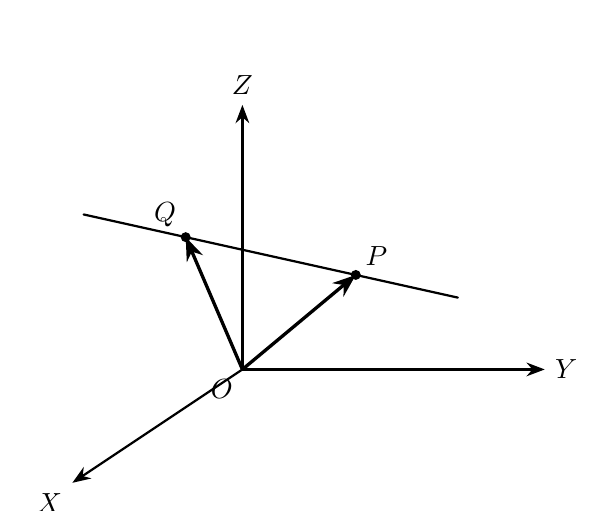
\begin{tikzpicture}[>=Stealth, scale=1.2, line cap=round, line join=round]
  % Coordinates axes
  \draw[->, thick] (0, 0) -- (-1.8, -1.2) node[below left] {$X$};
  \draw[->, thick] (0, 0) -- (3.2, 0) node[right] {$Y$};
  \draw[->, thick] (0, 0) -- (0, 2.8) node[above] {$Z$};
  \node[below left] at (0,0) {$O$};

  % Points P and Q
  \coordinate (P) at (1.2, 1.0);
  \coordinate (Q) at (-0.6, 1.4);

  % Draw OP and OQ
  \draw[->, very thick] (0,0) -- (P) node[midway, right=1pt] {};
  \draw[->, very thick] (0,0) -- (Q) node[midway, left=1pt] {};

  % Draw line through P and Q
  \draw[thick] ($(P)!-0.6!(Q)$) -- ($(P)!1.6!(Q)$);

  \fill (P) circle (1.5pt) node[above right] {$P$};
  \fill (Q) circle (1.5pt) node[above left] {$Q$};
\end{tikzpicture}
\caption*{圖 1-1}\label{fig:b6-1-1}
\end{figure}

在 $\mathbb{R}^3$ 中，可作圖如圖 1-1。

關於一般 $\mathbb{R}^n$ 中的“距離”以及相關的“垂直”等觀念，就不擬作深入討論了。

\subsubsection*{丙、線性相關與線性無關}\label{subsec:b6-1-1-c}

為了計算的方便，從本段開始我們一律不區分點與向量，而一律以圓括弧“$(\quad)$”表點和向量。

讓我們從一個例子開始：

\begin{example}\label{ex:b6-1-4}
$\mathbb{R}^3$ 中二向量 $\vec{OP}=(-1, 2, 1), \vec{OQ}=(3, -1, 3)$，試描出 $3\vec{OP}+2\vec{OQ}$ 的終點 $R$。
\end{example}

\paragraph{【解】}
在等價看法下
\[ R = (-3, 6, 3) + (6, -2, 6) = (3, 4, 9) \]

\begin{figure}[H]
\centering
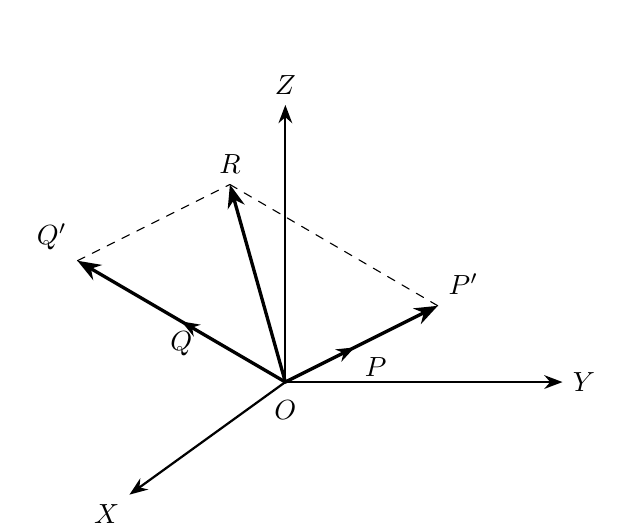
\begin{tikzpicture}[>=Stealth, scale=1.1, line cap=round, line join=round]
  % Axes
  \draw[->, thick] (0, 0) -- (-1.8, -1.3) node[below left] {$X$};
  \draw[->, thick] (0, 0) -- (3.2, 0) node[right] {$Y$};
  \draw[->, thick] (0, 0) -- (0, 3.2) node[above] {$Z$};
  \node[below] at (0, -0.1) {$O$};

  % Vectors P, Q, P', Q', R
  \coordinate (P) at (0.8, 0.4);
  \coordinate (Q) at (-1.2, 0.7);
  \coordinate (Pp) at ($(0,0)!2.2!(P)$);
  \coordinate (Qp) at ($(0,0)!2.0!(Q)$);
  \coordinate (R) at ($(Pp)+(Qp)$);

  \draw[->, thick] (0,0) -- (P) node[below right] {$P$};
  \draw[->, thick] (0,0) -- (Q) node[below] {$Q$};
  \draw[->, very thick] (0,0) -- (Pp) node[above right] {$P'$};
  \draw[->, very thick] (0,0) -- (Qp) node[above left] {$Q'$};
  \draw[->, very thick] (0,0) -- (R) node[above] {$R$};

  \draw[dashed] (Pp) -- (R);
  \draw[dashed] (Qp) -- (R);
\end{tikzpicture}
\caption*{圖 1-2}\label{fig:b6-1-2}
\end{figure}

讀者或能直觀地看出，在上例中 $R$ 是落在由 $O, P, Q$ 三點所決定的平面上。並且可以算出 $\vec{Q'R}=\vec{OP'}, \vec{P'R}=\vec{OQ'}$。反之，對 $O, P, Q$ 三點所決定平面上任一點如 $R$ 者，可以自 $R$ 聯平行線分別平行於 $\vec{OQ}$ 及 $\vec{OP}$，設分別交於 $Q', P'$，令 $\alpha = \frac{\overline{OP'}}{\overline{OP}}, \beta = \frac{\overline{OQ'}}{\overline{OQ}}$ 則 $\vec{OR} = \alpha\vec{OP} + \beta\vec{OQ}$，或作 $\vec{OR} - \alpha\vec{OP} - \beta\vec{OQ} = \vect{0}$。

例 4 提示了四件事：
\begin{enumerate}[label=(\alph*), leftmargin=2em]
  \item 對任意實數 $\alpha, \beta$，$\alpha\vec{OP} + \beta\vec{OQ}$ 均在 $O, P, Q$ 所決定的平面上。
  \item $O, P, Q$ 所張平面上任一點均可表作 $\alpha\vec{OP} + \beta\vec{OQ}$ 的形式。
  \item 對這平面上任一點 $R$，可找到實數 $\alpha, \beta, \gamma$ 使得 $\alpha\vec{OP} + \beta\vec{OQ} + \gamma\vec{OR} = \vect{0}$。
  \item 性質 (c) 並不對空間中其他點適合。
\end{enumerate}

現在要規定幾個重要名詞：設 $\vect{a}_1, \vect{a}_2, \dots, \vect{a}_m$ 為 $\mathbb{R}^n$ 中向量。

\begin{definition}\label{def:b6-1-1}
\begin{enumerate}[label=(\roman*), leftmargin=2em]
  \item 設向量 $\vect{b}$ 在 $\mathbb{R}^n$ 中可表作 $\vect{b}=\sum_{i=1}^m \lambda_i \vect{a}_i$（$\lambda_i$ 均為實數），則稱 $\vect{b}$ 為 $\vect{a}_1, \vect{a}_2, \dots, \vect{a}_m$ 的\textbf{線性組合}。
  \item $\sigma = \left\{ \vect{b} \;\middle|\; \vect{b}=\sum_{i=1}^m \lambda_i \vect{a}_i, \lambda_i \text{ 為實數} \right\}$ 稱為由 $\vect{a}_1, \vect{a}_2, \dots, \vect{a}_m$ 所\textbf{張成的子空間}。
\end{enumerate}
\end{definition}

由 (a) 式，$\vec{OP}, \vec{OQ}$ 所張成的子空間（在點與向量的等價看法下）就是過原點的一個平面，由 $\vec{OP}$ 所張成的子空間便是過原點的一條直線，顯然原點 $O$ 在這些子空間上。

\begin{discussion}\label{disc:b6-1-1}
向量 $\vect{u}=(-1, 2, 1), \vect{v}=(3, -1, 3)$ 展成的子空間設為 $\sigma$。令 $\vec{OP}=(x, y, z)$ 為子空間（平面）上一點，則存在實數 $\alpha, \beta$ 使得
\[ \vec{OP}=(x, y, z) = \alpha \vect{u} + \beta \vect{v} = (-\alpha+3\beta, 2\alpha-\beta, \alpha+3\beta) \]
即
\begin{equation}
\left\{\begin{aligned}
-\alpha + 3\beta &= x \\
2\alpha - \beta &= y \\
\alpha + 3\beta &= z
\end{aligned}\right. \label{eq:b6-1-1-6}
\end{equation}
由消去法解得
\begin{equation}
7x + 6y - 5z = 0 \label{eq:b6-1-1-7}
\end{equation}
即 $x, y, z$ 滿足 (7) 式。反之若 $\vec{OP}=(x, y, z)$ 滿足 (7) 式，則由 (6) 式求 $\alpha, \beta$：
\begin{enumerate}[label=(\roman*), leftmargin=2em]
  \item (6) 式可解，因為
  \[ \begin{vmatrix} -1 & 3 & x \\ 2 & -1 & y \\ 1 & 3 & z \end{vmatrix} = 7x + 6y - 5z = 0 \]
  \item 對此一組解 $\alpha, \beta$，顯然
  \[ \vec{OP} = (x, y, z) = \alpha\vect{u} + \beta\vect{v} \]
\end{enumerate}
這說明了 (7) 式為點 $\vec{OP}$ 在 $\vect{u}, \vect{v}$ 所展成子空間的充要條件，通稱為一平面的方程式。\hfill$\#$
\end{discussion}

\paragraph{附註：}雖然用一個數表示點的位置，古希臘時代就已經開始用了，並且到紀元 1637 年，笛卡爾把這個觀念推到二維和三維的情形，但直到十九世紀數學家 Cayley 和 Grassmann 才發現到“為什麼要停在三個數上呢？”這才開始了 $n$ 維空間的研究。

\subsubsection*{作業 1}\label{hw:b6-1-1}
設 $\vect{u}, \vect{v}$ 同上，
\begin{enumerate}[label=(\roman*), leftmargin=2em]
  \item $\vect{w}=(1, 1, 0)$，試問 $\vect{u}, \vect{v}, \vect{w}$ 所展成的子空間是否為一平面？
  \item 若 $\vect{w}$ 改成 $(3, 4, 9)$ 又如何？
\end{enumerate}

\begin{definition}\label{def:b6-1-2}
設 $\vect{a}_1, \vect{a}_2, \dots, \vect{a}_m$ 為 $\mathbb{R}^n$ 中向量，若存在非盡為 0 的實數 $\lambda_1, \lambda_2, \dots, \lambda_m$ 使得
\begin{equation}
\sum_{i=1}^m \lambda_i \vect{a}_i = \vect{0} \label{eq:b6-1-1-8}
\end{equation}
則稱 $\vect{a}_1, \vect{a}_2, \dots, \vect{a}_m$ 為\textbf{線性相關}。反之，對一組 $\lambda_1, \lambda_2, \dots, \lambda_m$，若 $\sum_{i=1}^m \lambda_i \vect{a}_i = \vect{0}$ 僅當 $\lambda_1=\lambda_2=\dots=\lambda_m=0$ 時成立，此時 $\vect{a}_1, \vect{a}_2, \dots, \vect{a}_m$ 稱作\textbf{線性無關}。
\end{definition}

由第三冊的討論，$\mathbb{R}^3$ 中可以找到三個線性無關的向量，而且 $\mathbb{R}^3$ 中線性無關向量的最大數是 3，並且任何向量均可唯一表成三個線性無關向量的線性組合，也就是說三個線性無關的向量形成 $\mathbb{R}^3$ 的一組基底，並且任何四向量在 $\mathbb{R}^3$ 中均線性相關。在 $\mathbb{R}^n$ 中我們有類似的性質，試條列數項於后，作為參考。至於嚴格的證明雖是不難但較繁瑣，就略去不提。讀者只要將 $\mathbb{R}^3$ 的情形弄清楚，以憑藉它來推想。
\begin{enumerate}[label=\Roman*., leftmargin=2.5em]
  \item $\mathbb{R}^n$ 中線性無關向量之最大數恰好是 $n$，並且 $\mathbb{R}^n$ 中任一向量均可表為 $n$ 個線性無關向量的線性組合。這樣一組 $n$ 個線性無關的向量稱作一組\textbf{基底}（顯然 $\vect{0}$ 不在內）。
  \item $\mathbb{R}^n$ 中的任 $k$ 個線性無關向量 $\vect{a}_1, \vect{a}_2, \dots, \vect{a}_k$，$k < n$，都可另找到 $\vect{a}_{k+1}, \dots, \vect{a}_n$，使得 $\vect{a}_1, \vect{a}_2, \dots, \vect{a}_n$ 為線性無關。
\end{enumerate}

\paragraph{註：}對一個基底，固定一點為基準點，I 中所說即此組基底形成一 $\mathbb{R}^n$ 中的座標系。

本書將恆以 $\vect{e}_1, \vect{e}_2, \dots, \vect{e}_n$ 為基底，原點 $O$ 為基準點形成的座標系來討論。

\begin{example}\label{ex:b6-1-5}
$\mathbb{R}^4$ 中試問 $\vect{u}_1=(1, 2, 0, 1), \vect{u}_2=(-1, 1, 1, 0), \vect{u}_3=(0, -1, 2, -3), \vect{u}_4=(3, 1, -1, 2)$ 是線性相關還是線性無關？
\end{example}

\paragraph{【解】}
設存在 $\lambda_1, \lambda_2, \lambda_3, \lambda_4$ 使得
\[ \lambda_1\vect{u}_1 + \lambda_2\vect{u}_2 + \lambda_3\vect{u}_3 + \lambda_4\vect{u}_4 = \vect{0} \]
即
\begin{equation}
\left\{\begin{aligned}
\lambda_1 - \lambda_2 \phantom{+ 2\lambda_3} + 3\lambda_4 &= 0 \\
2\lambda_1 + \lambda_2 - \lambda_3 + \lambda_4 &= 0 \\
\lambda_2 + 2\lambda_3 - \lambda_4 &= 0 \\
\lambda_1 \phantom{+ \lambda_2} - 3\lambda_3 + 2\lambda_4 &= 0
\end{aligned}\right. \label{eq:b6-1-1-9}
\end{equation}
若此聯立方程組有一組非全為 0 的解，則 $\vect{u}_1, \vect{u}_2, \vect{u}_3, \vect{u}_4$ 為線性相關，否則為線性無關。用消去法解之，發現此方程組只有一組 $\lambda_1=\lambda_2=\lambda_3=\lambda_4=0$ 的解，故 $\vect{u}_1, \vect{u}_2, \vect{u}_3, \vect{u}_4$ 為線性無關。\hfill$\#$

\begin{example}\label{ex:b6-1-6}
在上例中以 $\vect{u}_1, \vect{u}_2, \vect{u}_3, \vect{u}_4$ 的線性組合來表 $\vect{a}=(2, 2, -1, 6)$。
\end{example}

\paragraph{【解】}
此題在於找 $\lambda_1, \lambda_2, \lambda_3, \lambda_4$ 使得
\[ \lambda_1\vect{u}_1 + \lambda_2\vect{u}_2 + \lambda_3\vect{u}_3 + \lambda_4\vect{u}_4 = \vect{a} \]
由向量相等的意義得聯立方程：
\begin{equation}
\left\{\begin{aligned}
\lambda_1 - \lambda_2 \phantom{+ 2\lambda_3} + 3\lambda_4 &= 2 \\
2\lambda_1 + \lambda_2 - \lambda_3 + \lambda_4 &= 2 \\
\lambda_2 + 2\lambda_3 - \lambda_4 &= -1 \\
\lambda_1 \phantom{+ \lambda_2} - 3\lambda_3 + 2\lambda_4 &= 6
\end{aligned}\right. \label{eq:b6-1-1-10}
\end{equation}
用消去法得 $\lambda_1=1, \lambda_2=2, \lambda_3=-1, \lambda_4=1$。故
\[ \vect{a} = \vect{u}_1 + 2\vect{u}_2 - \vect{u}_3 + \vect{u}_4 \]\hfill$\#$

上例中 $\lambda_1, \lambda_2, \lambda_3, \lambda_4$ 不難解得，但一般情形如何？請就以下作業試驗。

\subsubsection*{作業 2}\label{hw:b6-1-2}
$\vect{u}_1, \vect{u}_2, \vect{u}_3$ 同上，問能否用三向量的線性組合表 $\vect{a}=(1, 1, -\frac{1}{2}, 3)$？這說明什麼？

\subsubsection*{作業 3}\label{hw:b6-1-3}
$\vect{u}_1, \vect{u}_2, \vect{u}_3$ 同上，$\vect{u}_4$ 改為 $(3, 2, 1, -1)$ 則四向量能否表 $\vect{a}=(1, 1, -\frac{1}{2}, 3)$？為什麼？

\paragraph{註：}關於一般 $n$ 元一次聯立方程的公式解，請參考 § I-8 的討論。至於消去法，讀者應已很熟練了。

\begin{theorem}\label{thm:b6-1-1}
$\vect{a}_1, \vect{a}_2, \dots, \vect{a}_m$ 為線性相關，則必其中某一向量可寫為其餘諸向量的線性組合，即在其餘諸向量所決定的子空間上。
\end{theorem}

\begin{proof}[【證明】]
由假設，可找到非盡為 0 的 $\lambda_1, \lambda_2, \dots, \lambda_m$ 使得 (8) 式成立。經重新安排指標可假設 $\lambda_1 \ne 0$，則
\[ \lambda_1 \vect{a}_1 = - \sum_{i=2}^m \lambda_i \vect{a}_i \]
即
\[ \vect{a}_1 = \sum_{i=2}^m \left(-\dfrac{\lambda_i}{\lambda_1}\right) \vect{a}_i \]
\end{proof}\hfill$\#$

\subsubsection*{作業 4}\label{hw:b6-1-4}
試證 $\vect{e}_1, \vect{e}_2, \dots, \vect{e}_n$ 在 $\mathbb{R}^n$ 中形成一組基底。（即證：\textcircled{1} $\vect{e}_1, \vect{e}_2, \dots, \vect{e}_n$ 線性無關。\textcircled{2} $\mathbb{R}^n$ 中任一向量均可寫成此 $n$ 個向量的線性組合。）

\subsubsection*{作業 5}\label{hw:b6-1-5}
在 $\mathbb{R}^5$ 中，將 $\vect{a}=(4, 61, -13, 7, 9)$ 寫作其第一至第五個單位向量的線性組合。此寫法是否唯一？說明之。

\subsubsection*{作業 6}\label{hw:b6-1-6}
$\mathbb{R}^3$ 中設 $\vect{a}_1=(1, 2, 1), \vect{a}_2=(2, -1, 3), \vect{a}_3=(-1, 1, 1)$。
\begin{enumerate}[label=(\roman*), leftmargin=2em]
  \item 試證 $\vect{a}_1, \vect{a}_2, \vect{a}_3$ 線性無關。
  \item 若 $\vect{a}=(3, 4, 2)$，試將 $\vect{a}$ 寫作 $\vect{a}_1, \vect{a}_2, \vect{a}_3$ 的線性組合。
  \item 試證不可能找到一向量 $\vect{a}_4$，使得 $\vect{a}_1, \vect{a}_2, \vect{a}_3, \vect{a}_4$ 線性無關。
\end{enumerate}

\subsubsection*{作業 7}\label{hw:b6-1-7}
$\mathbb{R}^3$ 中，試證不可能找到向量 $\vect{a}_1, \vect{a}_2$，使得 $\mathbb{R}^3$ 中任何一向量均可寫成它們的線性組合。

\subsubsection*{作業 8}\label{hw:b6-1-8}
設 $\vect{a}_1=(1, 2, 4), \vect{a}_2=(-1, 1, 3)$ 試找一 $\vect{a}_3$ 使得 $\vect{a}_1, \vect{a}_2, \vect{a}_3$ 為線性無關。（提示：方法很多，這種 $\vect{a}_3$ 也有無限個，只要找一向量不在 $\vect{a}_1, \vect{a}_2$ 所展成的子空間即可。）

\begin{definition*}[*]\label{def:b6-1-dim}
設 $\sigma$ 為 $\mathbb{R}^n$ 的一個子空間，$\sigma$ 中線性無關向量的最大數 $m$ 稱作 $\sigma$ 的\textbf{維數}，$\sigma$ 稱作 \textbf{$m$ 維子空間}\footnote{【原書註】：嚴格說，此定義不完全，有一個問題存在：此所謂的線性無關向量的最大數 $m$，會不會因兩次不同的向量取法而有不同？即是否有此 $m$ 存在？事實上與丙段 I, II 的情形一樣，下面幾個性質成立：
\begin{enumerate}[label=(\roman*), leftmargin=2em]
  \item 此 $m$ 存在。
  \item 任一 $\sigma$ 中的向量均可唯一寫成 $\sigma$ 中一組給定 $m$ 個線性無關向量的線性組合。
  \item 對 $\sigma$ 中任 $k$ 個線性無關的向量（$k < m$），可找到 $m-k$ 個向量使此 $m$ 個向量線性無關。
\end{enumerate}
因此我們也往往稱一個 $m$ 維子空間內，$m$ 個線性無關向量為一組基底。}。例如論例 1 之 $\sigma$ 為二維子空間。
\end{definition*}

\subsubsection*{作業 9}\label{hw:b6-1-9}
\begin{enumerate}[label=(\roman*), leftmargin=2em]
  \item 試求作業 1 中兩子空間的維數。
  \item 試求由 $\vect{u}=(-1, 2, 1)$ 與 $\vect{v}=(2, -4, -2)$ 所展成子空間方程式。（提示：為二方程式所組成。）
  \item 將 (ii) 中的直線用 (1) 式表出。
\end{enumerate}

從定義我們可以顯然看出，$\mathbb{R}^3$ 中三個向量若是線性相關，則三向量所決定的子空間必為一平面或為一直線或竟為 $O$ 點，即其維數必小於 3。

\subsubsection*{丁、$\mathbb{R}^n$ 中的線性映射與方陣}\label{subsec:b6-1-1-d}

$\mathbb{R}^n$ 顯然是人類最不難了解的空間，從 $\mathbb{R}^n$ 到 $\mathbb{R}^m$ 的函數當然也是最有趣的了。可是從 $\mathbb{R}^n$ 到 $\mathbb{R}^m$ 的函數一般來說是相當複雜的，其最有用的，也是人類最能處理的，就是一次的，也就是我們所稱\textbf{線性映射}了。我們將看出它與多元一次聯立方程組是息息相關的。為了討論方便，本書將僅討論 $n=m$ 的情形\footnote{【原書註】：二次方程也是人類較能了解的，但到了三次以上就非常艱深了。}。

在第四冊 § 1-3, § 1-4, § 1-5 內我們已經探討了 $\mathbb{R}^2$ 上的線性映射和它們的方陣表示。那邊特別舉出（平面上）剛性運動，強調某種線性映射相當於一種運動。或者我們更可以把線性映射看作經過一個三稜鏡或是放大鏡或是近視眼鏡所成的像來想像。

\begin{example}\label{ex:b6-1-7}
設 $f(x_1, x_2) = (\sqrt{3}x_1 - x_2, x_1 + \sqrt{3}x_2)$，試求點 $O(0, 0)$，$A(1, 1), B(0, 2), C(-1, 1)$ 的像點 $O, A', B', C'$ 的座標，又 $O, A, B, C$ 形成一正方形的四端點，是否 $O, A', B', C'$ 亦形成一正方形的四端點？
\end{example}

\paragraph{【解】}
$A'=(\sqrt{3}-1, 1+\sqrt{3})$，$B'=(-2, 2\sqrt{3})$，$C'=(-\sqrt{3}-1, -1+\sqrt{3})$。
又驗證 $\vec{OA'} \cdot \vec{OC'} = \vec{A'B'} \cdot \vec{B'C'} = \vec{B'C'} \cdot \vec{OC'} = 0$
且 $\overline{OA'} = \overline{A'B'} = \overline{B'C'} = \overline{OC'} = 2\sqrt{2}$。
所以 $O, A', B', C'$ 形成正方形的端點，而且邊界映射到相應邊界，（$\mathbb{R}^2$ 中線性映射將直線映到直線）。只是邊長改變了兩倍，位置也不一樣了，反時針轉了 $\dfrac{\pi}{6}$，見圖 1-3。\hfill$\#$

\begin{figure}[H]
\centering
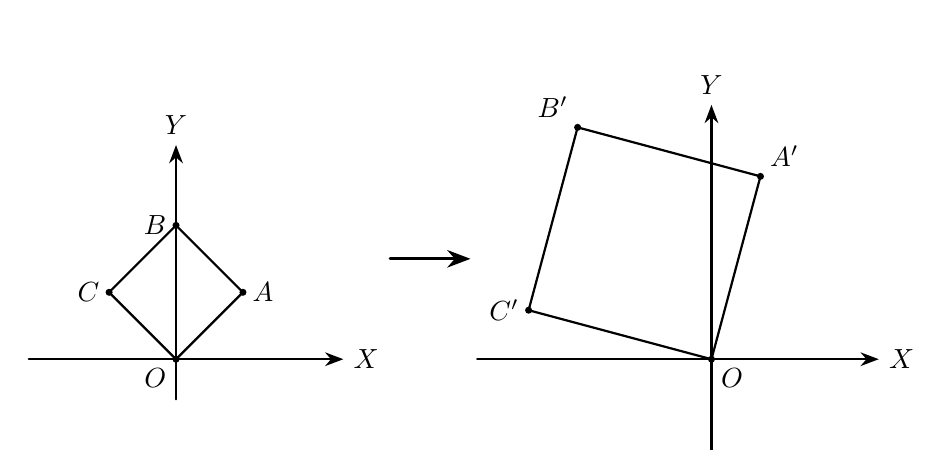
\begin{tikzpicture}[>=Stealth, scale=0.85, line cap=round, line join=round]
  % Left figure
  \begin{scope}[shift={(0,0)}]
    \draw[->, thick] (-2.2, 0) -- (2.5, 0) node[right] {$X$};
    \draw[->, thick] (0, -0.6) -- (0, 3.2) node[above] {$Y$};
    \node[below left] at (0,0) {$O$};

    \coordinate (O) at (0,0);
    \coordinate (A) at (1,1);
    \coordinate (B) at (0,2);
    \coordinate (C) at (-1,1);

    \draw[thick] (O) -- (A) -- (B) -- (C) -- cycle;
    \fill (O) circle (1.5pt);
    \fill (A) circle (1.5pt) node[right] {$A$};
    \fill (B) circle (1.5pt) node[left] {$B$};
    \fill (C) circle (1.5pt) node[left] {$C$};
  \end{scope}

  % Mapping arrow
  \draw[->, very thick] (3.2, 1.5) -- (4.4, 1.5);

  % Right figure
  \begin{scope}[shift={(8,0)}]
    \draw[->, thick] (-3.5, 0) -- (2.5, 0) node[right] {$X$};
    \draw[->, thick] (0, -1.5) -- (0, 3.8) node[above] {$Y$};
    \node[below right] at (0,0) {$O$};

    \coordinate (O) at (0,0);
    \coordinate (Ap) at ({sqrt(3)-1}, {1+sqrt(3)});
    \coordinate (Bp) at (-2, {2*sqrt(3)});
    \coordinate (Cp) at ({-sqrt(3)-1}, {-1+sqrt(3)});

    \draw[thick] (O) -- (Ap) -- (Bp) -- (Cp) -- cycle;
    \fill (O) circle (1.5pt);
    \fill (Ap) circle (1.5pt) node[above right] {$A'$};
    \fill (Bp) circle (1.5pt) node[above left] {$B'$};
    \fill (Cp) circle (1.5pt) node[left] {$C'$};
  \end{scope}
\end{tikzpicture}
\caption*{圖 1-3}\label{fig:b6-1-3}
\end{figure}

\subsubsection*{作業 10}\label{hw:b6-1-10}
上例 $f$ 的方陣表示為何？是否為一剛性運動？

\subsubsection*{作業 11}\label{hw:b6-1-11}
試求正方形 $OABC$（包括邊界和內部）的映像為何？說明之。

\paragraph{注意：}關於列出一線性映射之方陣及一點座標而求像點，我們可將點座標寫在左邊，方陣寫在右邊，然後以點座標的列乘以方陣的行即得。就如：
\[ (x_1, x_2) \begin{pmatrix} a_{11} & a_{12} \\ a_{21} & a_{22} \end{pmatrix} \]
相乘有如：
\[ (\longrightarrow) \begin{pmatrix} \Big\downarrow & \Big\downarrow \end{pmatrix} \]

\begin{example}\label{ex:b6-1-8}
設 $f$ 的方陣表示為 $\begin{pmatrix} 2 & 1 \\ 1 & -1 \end{pmatrix}$，$O, A, B, C$ 同上，$A', B', C'$ 分別為 $f$ 下的像點，求其座標。四邊形 $OA'B'C'$ 是否成一正方形？
\end{example}

\paragraph{【解】}
\begin{align*}
A' &= (1, 1) \begin{pmatrix} 2 & 1 \\ 1 & -1 \end{pmatrix} = (2+1, 1-1) = (3, 0) \\
B' &= (0, 2) \begin{pmatrix} 2 & 1 \\ 1 & -1 \end{pmatrix} = (2, -2) \\
C' &= (-1, 1) \begin{pmatrix} 2 & 1 \\ 1 & -1 \end{pmatrix} = (-2+1, -1-1) = (-1, -2)
\end{align*}
$\vec{OA'} \cdot \vec{OC'} = -3 \ne 0$。
故此四邊形非正方形。由於線性映射把向量映至向量，也就是說，把相平行的線段映至相平行的線段，所以四邊形 $OA'B'C'$ 為平行四邊形。當然這也可以由直接檢視向量 $\vec{OA'}=\vec{C'B'}, \vec{A'B'}=\vec{OC'}$ 得知。見圖 1-4。\hfill$\#$

\begin{example}\label{ex:b6-1-9}
設 $f$ 之方陣表示為 $\begin{pmatrix} 1 & -2 \\ 2 & -4 \end{pmatrix}$，$O, A, B, C$ 同上，求 $A', B', C'$ 之座標。
\end{example}

\paragraph{【解】}
同上計算得
\[ A'=(3, -6), \quad B'=(4, -8), \quad C'=(1, -2) \]
且
\[ \begin{vmatrix} 3 & -6 & 1 \\ 4 & -8 & 1 \\ 1 & -2 & 1 \end{vmatrix} = 0 \]
三點共線。見圖 1-5。\hfill$\#$

\begin{figure}[H]
\centering
\begin{minipage}[c]{0.48\textwidth}
\centering
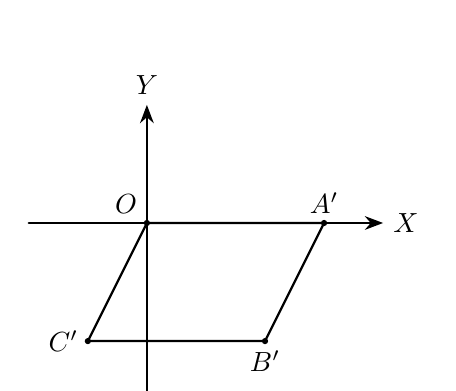
\begin{tikzpicture}[>=Stealth, scale=0.75, line cap=round, line join=round]
  \draw[->, thick] (-2.0, 0) -- (4.0, 0) node[right] {$X$};
  \draw[->, thick] (0, -3.0) -- (0, 2.0) node[above] {$Y$};
  \node[above left] at (0,0) {$O$};

  \coordinate (O) at (0,0);
  \coordinate (Ap) at (3,0);
  \coordinate (Bp) at (2,-2);
  \coordinate (Cp) at (-1,-2);

  \draw[thick] (O) -- (Ap) -- (Bp) -- (Cp) -- cycle;
  \fill (O) circle (1.5pt);
  \fill (Ap) circle (1.5pt) node[above] {$A'$};
  \fill (Bp) circle (1.5pt) node[below] {$B'$};
  \fill (Cp) circle (1.5pt) node[left] {$C'$};
\end{tikzpicture}
\caption*{圖 1-4}\label{fig:b6-1-4}
\end{minipage}\hfill
\begin{minipage}[c]{0.48\textwidth}
\centering
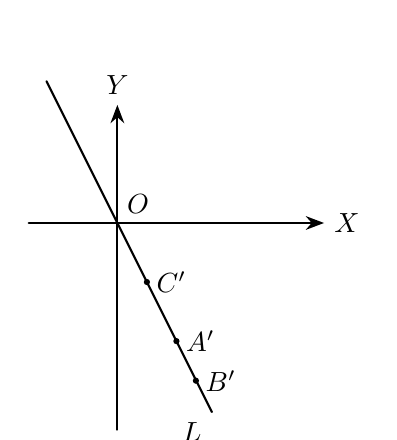
\begin{tikzpicture}[>=Stealth, scale=0.75, line cap=round, line join=round]
  \draw[->, thick] (-1.5, 0) -- (3.5, 0) node[right] {$X$};
  \draw[->, thick] (0, -3.5) -- (0, 2.0) node[above] {$Y$};
  \node[above right] at (0,0) {$O$};

  % Line L: 2x + y = 0
  \draw[thick] (-1.2, 2.4) -- (1.6, -3.2) node[below left] {$L$};

  \coordinate (Cp) at (0.5, -1.0);
  \coordinate (Ap) at (1.0, -2.0);
  \coordinate (Bp) at (1.33, -2.67);

  \fill (Cp) circle (1.5pt) node[right] {$C'$};
  \fill (Ap) circle (1.5pt) node[right] {$A'$};
  \fill (Bp) circle (1.5pt) node[right] {$B'$};
\end{tikzpicture}
\caption*{圖 1-5}\label{fig:b6-1-5}
\end{minipage}
\end{figure}

\subsubsection*{作業 12}\label{hw:b6-1-12}
試證在例 9 中，整個 $\mathbb{R}^2$ 平面映成到直線 $L$。

從上三例約略可以窺見，平面上一般的線性映射是相當複雜的也不像剛性運動那樣規則。一般 $\mathbb{R}^n$ 到 $\mathbb{R}^n$ 的線性映射亦可類似定義，不過在 $n \ge 3$ 時其構造又自然複雜多了。本章主要目的在闡明線性映射及其方陣之表示與行列式有關的基本重要問題。

\begin{definition}\label{def:b6-1-3}
設有一函數 $f: \mathbb{R}^n \longrightarrow \mathbb{R}^n$，若 $(y_1, y_2, \dots, y_n)$ 表示點 $(x_1, x_2, \dots, x_n)$ 在 $f$ 下的像點，即 $f(x_1, x_2, \dots, x_n) = (y_1, y_2, \dots, y_n)$，而知存在 $n^2$ 個實數 $a_{ij}$，$i, j = 1, 2, \dots, n$ 使得
\begin{equation}
y_j = \sum_{i=1}^n a_{ij} x_i \qquad j = 1, 2, \dots, n \label{eq:b6-1-1-11}
\end{equation}
對每一點 $(x_1, x_2, \dots, x_n)$ 均成立，則稱 $f$ 為 $\mathbb{R}^n$ 到 $\mathbb{R}^n$ 的一個\textbf{線性映射}。
\end{definition}

通常 $f$ 可記為
\[ f(x_1, x_2, \dots, x_n) = \left( \sum_{i=1}^n a_{i1} x_i, \sum_{i=1}^n a_{i2} x_i, \dots, \sum_{i=1}^n a_{in} x_i \right) \]
這 $n^2$ 個實數 $a_{ij}$ 形成一個正方形的矩陣，稱作 \textbf{$n$ 階方陣}，記為
\begin{equation}
\begin{pmatrix}
a_{11} & a_{12} & \dots & a_{1n} \\
a_{21} & a_{22} & \dots & a_{2n} \\
\dots & \dots & \dots & \dots \\
a_{n1} & a_{n2} & \dots & a_{nn}
\end{pmatrix} \quad \text{或簡記作 } (a_{ij}) \label{eq:b6-1-1-12}
\end{equation}
其中 $a_{ij}$ 稱為原素，各橫列稱作方陣之\textbf{列}，各縱行稱作方陣之\textbf{行}，$a_{ij}$ 係位於第 $i$ 列第 $j$ 行的原素，$i$ 稱作列指標，$j$ 稱作行指標。方陣之各原素均有一定位置，兩方陣僅在對應位置之各原素均相等時，始稱相等。顯然 $\mathbb{R}^n$ 到 $\mathbb{R}^n$ 的線性映射與 $n$ 階方陣之間有一一對應的關係，即兩線性映射為相等當且僅當對應之方陣相等。相應於每一線性映射有一方陣，對每一方陣可找唯一線性映射使彼之方陣表示即為此給定方陣。

以方陣之第 $i$ 列中各原素作分量而得之向量
\begin{equation}
\vect{a}_i = (a_{i1}, a_{i2}, \dots, a_{in}) \qquad i=1, 2, \dots, n \label{eq:b6-1-1-13}
\end{equation}
稱作方陣之第 $i$ 個\textbf{列向量}，以第 $j$ 行的各原素為分量而得之向量
\begin{equation}
\vect{a}_j^* = (a_{1j}, a_{2j}, \dots, a_{nj}) \qquad j=1, 2, \dots, n \label{eq:b6-1-1-14}
\end{equation}
稱作方陣之第 $j$ 個\textbf{行向量}。

\begin{example}\label{ex:b6-1-10}
設 $f(x_1, x_2, x_3) = (3x_1 - 2x_2 + x_3, x_1 + x_2 - x_3, x_1 + 2x_2 - 2x_3)$ 問 $f$ 是否線性映射？若是，其方陣表示為何？又求 $P(1, 2, 1), Q(2, 1, -1), R(3, 0, -3)$ 相應之像點 $P', Q', R'$ 的座標。又知 $P, Q, R$ 三點在一直線上（因為 $\vec{OR} = \vec{OP} + 2\vec{PQ}$）問 $P', Q', R'$ 是否也在同一直線上？
\end{example}

\paragraph{【解】}
$f$ 之方陣表示為
\[ \begin{pmatrix} 3 & 1 & 1 \\ -2 & 1 & 2 \\ 1 & -1 & -2 \end{pmatrix} \]
\begin{align*}
P' &= (1, 2, 1) \begin{pmatrix} 3 & 1 & 1 \\ -2 & 1 & 2 \\ 1 & -1 & -2 \end{pmatrix} = (3-4+1, 1+2-1, 1+4-2) = (0, 2, 3)
\end{align*}
同理 $Q' = (3, 4, 6)$，$R' = (6, 6, 9)$。
且 $\vec{OR'} = \vec{OP'} + 2\vec{P'Q'}$，故 $P', Q', R'$ 在同一直線上。

另一種看法是：$P', Q', R'$ 在同一直線上的充要條件是 $\vec{P'Q'}$ 與 $\vec{P'R'}$ 線性相關，這是極易判定的。\hfill$\#$

\subsubsection*{作業 13}\label{hw:b6-1-13}
試證線段 $OP$ 在 $f$ 下的映像為線段 $OP'$。

\subsubsection*{作業 14}\label{hw:b6-1-14}
設 $f: \mathbb{R}^3 \longrightarrow \mathbb{R}^3$ 定為 $f(x_1, x_2, x_3) = (x_1 + 2x_2^2, -x_3, x_2 - x_3)$，
$g: \mathbb{R}^3 \longrightarrow \mathbb{R}^3$ 定為 $g(x_1, x_2, x_3) = (x_1 x_2, x_1 + x_3, x_2 - x_3)$。
試問 $f, g$ 是否為線性映射？說明之。

\subsubsection*{作業 15}\label{hw:b6-1-15}
$f$ 如例 10 所示，設 $S=(3, 3, 0)$ 我們知 $\vec{OP} = \vec{QS}$（亦即 $OP \parallel QS$）試證 $OP' \parallel Q'S'$，$S'=f(S)$，又試證 $\vec{OP'} = \vec{Q'S'}$。

線性映射顯然把原點映至原點，作業 13 與 15 的性質事實上對一般線性映射均成立。線性映射原是一個把 $\mathbb{R}^n$ 的點指向其像點的函數，我們也可將之看作是從向量映到向量的函數，關係如下：
\[ f(P)=P' \text{ 可記為 } f(\vec{OP}) = \vec{OP'} \]
也就是在點與向量的等價關係下，把線性映射 $f: \mathbb{R}^n \longrightarrow \mathbb{R}^n$ 也看作是由 $\mathbb{R}^n$ 中的向量映到 $\mathbb{R}^n$ 中向量的函數。這樣，對 $\mathbb{R}^n$ 中向量 $\vect{a}$，$f(\vect{a})$ 就有意義了。即設 $\vect{a}=\vec{OA}$，則 $f(\vect{a}) = f(A)$（見作業 13）。在此種等價關係下，容易驗證 $\mathbb{R}^n$ 上的線性映射 $f$ 滿足：
\begin{enumerate}[label=\Roman*., leftmargin=2.5em]
  \item 對所有向量 $\vect{a}, \vect{b}$ 和實數 $\alpha, \beta$ 均成立：
  \begin{equation}
  f(\alpha\vect{a} + \beta\vect{b}) = \alpha f(\vect{a}) + \beta f(\vect{b}) \label{eq:b6-1-1-15}
  \end{equation}
  \item $f$ 把直線映至直線。
  \item 設 $f$ 如 (11) 給定，$\vect{e}_1, \vect{e}_2, \dots, \vect{e}_n$ 如前，則
  \begin{equation}
  f(\vect{e}_i) = \sum_{j=1}^n a_{ij} \vect{e}_j \label{eq:b6-1-1-16}
  \end{equation}
  （請注意 (16) 與 (11) 中指標次序不同）
  \item $f$ 把線性相關向量映至線性相關向量。
\end{enumerate}

\paragraph{注意：}$f$ 不一定將線性無關向量映至線性無關向量，參考例 9。

\subsubsection*{作業 16}\label{hw:b6-1-16}
試證對 $\mathbb{R}^n$ 中任意四點 $P_1, P_2, Q_1, Q_2$ 若有 $\vec{P_1P_2} = \vec{Q_1Q_2}$ 則 $f(\vec{P_1P_2}) = f(\vec{Q_1Q_2})$（提示：由 (11) 式或 (15) 式）。

\subsubsection*{作業 17}\label{hw:b6-1-17}
試證明上面 I, II, III, IV 諸性質。

\subsubsection*{習題 I-1}\label{sec:b6-ex1-1}

\begin{enumerate}[label=\arabic*., leftmargin=2em]
  \item $\mathbb{R}^3$ 中二向量 $\left(\dfrac{1}{2}, -3, 5\right)$ 與 $(1, -6, 10)$ 是否平行？

  \stepcounter{enumi}
  \item[\textbf{*2.}] 過兩點 $\vec{OP}=(a_1, a_2, \dots, a_n), \vec{OQ}=(b_1, b_2, \dots, b_n)$ 的直線方程式可表為（亦即向量表示法）
  \phantomsection\label{note:b6-ch1-p19-l-eq}%
  \[ L = \{ \vec{OP} + \lambda\vec{PQ} : \lambda \text{ 為任意實數} \}\footnotemark \]
  \footnotetext{【原書校訂】：原書此處印作「$L=\{\vec{OP}+\lambda\vec{OQ}\}$」，據後文「$x_i = a_i + \lambda(b_i - a_i)$」校訂為方向向量 $\vec{PQ}$。}
  即 $(x_1, x_2, \dots, x_n)$ 為 $L$ 上一點的充要條件是存在一實數 $\lambda$，使得
  \[ x_i = a_i + \lambda(b_i - a_i) \qquad i=1, 2, \dots, n \]
  即
  \[ \dfrac{x_i - a_i}{b_i - a_i} = \lambda \qquad i=1, 2, \dots, n \]
  其中 $\lambda$ 隨點 $(x_1, x_2, \dots, x_n)$ 而變。所以直線方程式的另一種寫法為：
  \[ \dfrac{x_1 - a_1}{c_1} = \dfrac{x_2 - a_2}{c_2} = \dots = \dfrac{x_n - a_n}{c_n} \]
  $(c_1, c_2, \dots, c_n)$ 為與直線平行的一個向量，此稱直線的比例式。試求 $\mathbb{R}^3$ 中，過兩點 $(-5, 3, 2), (2, -3, 6)$ 的直線方程式的兩種寫法。\\
  （註：我們還可將 $\mathbb{R}^3$ 中直線方程式寫作兩平面方程式的交點，以後再作說明，請參考第三冊 § 4-8 之習題 8。）

  \item 設 $\vect{a}_1=(7, 1, -3), \vect{a}_2=(1, -5, 2)$ 試找 $\mathbb{R}^3$ 中一與 $\vect{a}_1, \vect{a}_2$ 線性無關的向量，並敘述理由。

  \item 如上題，找 $\mathbb{R}^3$ 中一點，使不在 $\vect{a}_1, \vect{a}_2$ 所決定的平面，並請敘述理由。

  \item 求 $\mathbb{R}^3$ 中由 $\vect{u}=(1, 2, -1), \vect{v}=(-1, 2, 2)$ 所決定平面之方程式表示。

  \item 設 $\mathbb{R}^3$ 中三點 $P_1=(1, 3, 6), P_2=(3, 4, -3), P_3=(2, 1, 5)$ 試決定下列向量：
  \begin{enumerate}[label=(\Alph*)]
    \item $\vec{OP_1} + \vec{OP_2} - \vec{OP_3}$
    \item $7\vec{OP_1} - 2\vec{OP_2} - 3\vec{OP_3}$
  \end{enumerate}

  \item 設 $P_1=(1, 1, 1), P_2=(0, 1, 1), P_3=(1, -1, 0)$ 為 $\mathbb{R}^3$ 中三點，$\vec{OP_4} = x\vec{OP_1} + y\vec{OP_2} + z\vec{OP_3}$。
  \begin{enumerate}[label=(\alph*)]
    \item 試決定 $\vec{OP_4}$ 的分量。
    \item 若 $P_4=O$ 試證 $x=y=z=0$ 為唯一解。
    \item $P_4=(1, 2, 3)$ 試求 $x, y, z$。
  \end{enumerate}

  \item 設 $P_1=(1, 1, 1, 0), P_2=(0, 1, 1, 1), P_3=(1, 1, 0, 0)$ 為 $\mathbb{R}^4$ 中三個點，且 $P_4 = x P_1 + y P_2 + z P_3$。
  \begin{enumerate}[label=(\alph*)]
    \item 試決定 $P_4$ 的分量。
    \item 若 $P_4=O$，試證 $x=y=z=0$。
    \item 若 $P_4=(1, 5, 3, 4)$ 試求 $x, y, z$。
    \item 請問可選擇到 $x, y, z$ 使得 $P_4=(1, 2, 3, 4)$ 可表成 $P_4 = x P_1 + y P_2 + z P_3$ 嗎？
  \end{enumerate}

  \stepcounter{enumi}
  \item[\textbf{*9.}] 設 $P=(x_1, x_2, \dots, x_n), Q=(y_1, y_2, \dots, y_n)$ 為 $\mathbb{R}^n$ 中二點，試問：
  \begin{enumerate}[label=(\alph*)]
    \item 如何描述 $QP$？
    \item $QP$ 與 $PQ$ 的關係如何？
  \end{enumerate}

  \item $P, Q$ 如上題，又如
  \[ PQ = \{ (z_1, z_2, \dots, z_n) : \text{存在一實數 } \lambda, \text{使得 } z_i = x_i + \lambda(y_i - x_i), i=1, 2, \dots, n \} \]
  則：
  \begin{enumerate}[label=(\alph*)]
    \item 如何描述 $QP$？
    \item $PQ$ 與 $QP$ 之關係如何？
  \end{enumerate}

  \item 設 $P, Q$ 為 $\mathbb{R}^5$ 中二點，且 $\vec{PQ} = (2, -3, -1, 0, 4)$。
  \begin{enumerate}[label=(\alph*)]
    \item 若 $P=(-1, 1, 0, -3, 7)$ 試求 $Q$ 點。
    \item 若 $Q=(-2, 3, -3, 2, 1)$ 試求 $P$ 點。
  \end{enumerate}

  \item 設 $P, Q$ 為 $\mathbb{R}^4$ 中二點，當 $P, Q$ 為下列各種情形時，試求 $\vec{PQ}, 2\vec{PQ}$ 及 $\vec{PQ}$ 方向的單位向量：
  \begin{enumerate}[label=(\alph*)]
    \item $P=(1, 0, 1, 1) \quad Q=(0, 1, 1, 0)$
    \item $P=(3, 2, 1, 0) \quad Q=(0, 1, 2, 3)$
  \end{enumerate}

  \item 設 $P, Q, R, S$ 為 $\mathbb{R}^3$ 中四點，若 $\vec{PQ} = \vec{RS}$，試問線段 $PQ$ 與 $RS$ 之間的關係如何？四邊形 $PQSR$ 的形狀如何？

  \item
  \begin{enumerate}[label=(\alph*)]
    \item 設 $P, Q, R, S$ 為 $\mathbb{R}^3$ 中四點，則如何可知四邊形 $PQRS$ 為一平行四邊形？
    \item 若 $P=(1, 0, -1), Q=(0, 1, 1), R=(1, 1, 0)$ 且 $PQRS$ 為一平行四邊形，試求 $S$ 點。
  \end{enumerate}

  \item 當 $\vect{a}_1, \vect{a}_2, \vect{a}_3$ 為下列各種情形時，試問 $\vect{a}_1, \vect{a}_2, \vect{a}_3$ 是否線性無關？
  \begin{enumerate}[label=(\alph*)]
    \item $\vect{a}_1=(1, 0, 1), \vect{a}_2=(0, 0, 1), \vect{a}_3=(1, 1, 1)$
    \item $\vect{a}_1=(1, -1, 2), \vect{a}_2=(7, 2, -1), \vect{a}_3=(-19, -8, 7)$
    \item $\vect{a}_1=(0, 2, -1), \vect{a}_2=(3, 0, -2), \vect{a}_3=(3, 2, 3)$
  \end{enumerate}

  \stepcounter{enumi}
  \item[\textbf{*16.}] 設 $\vect{a}_1,$ $\vect{a}_2,$ $\dots,$ $\vect{a}_n$ 為線性無關，且 $\vect{a}_{n+1}$ 非 $\vect{a}_1,$ $\vect{a}_2,$ $\dots,$ $\vect{a}_n$ 的線性組合。試證 $\vect{a}_1,$ $\vect{a}_2,$ $\dots,$ $\vect{a}_{n+1}$ 為線性無關。

  \stepcounter{enumi}
  \item[\textbf{**17.}] 試問下列 $\mathbb{R}^n$ 的各子集合中那些形成（向量）子空間？
  \begin{enumerate}[label=(\alph*)]
    \item $\{ (x_1, x_2, \dots, x_n) : x_1 \ge x_2 \}$
    \item $\{ (x_1, x_2, \dots, x_n) : 2x_1 - x_n = 0 \}$
    \item $\{ (x_1, x_2, \dots, x_n) : x_n \text{ 為整數} \}$
    \item $\{ (x_1, x_2, \dots, x_n) : x_n = 0 \}$
    \item $\{ (x_1, x_2, \dots, x_n) : f(t) = x_1 + x_2 t + \dots + x_n t^{n-1}, f(2) = 0 \}$
  \end{enumerate}

  \item 試求二向量 $(a, b), (c, d)$ 為線性無關的充要條件。

  \item 試求向量 $(a_1, a_2, a_3), (b_1, b_2, b_3), (c_1, c_2, c_3)$ 為線性無關的充要條件。

  \item 試證 $\vect{a}=(3, 1, 5), \vect{b}=(-2, 1, 3), \vect{c}=(19, -2, 0)$ 三向量為線性相關，並以 $\vect{a}, \vect{b}$ 的線性組合表 $\vect{c}$。

  \item 試求由向量 $\left(2, -\dfrac{1}{2}, 3\right)$ 過點 $(1, -1, 1)$ 所決定的直線的方程式。

  \item $f(x_1, x_2, x_3) = (3x_1 - x_2 + 2x_3, x_1 - 3x_2 - x_3, 2x_1 + x_2 + 3x_3)$ 試求 $f$ 之方陣表示。設 $\vect{e}_1, \vect{e}_2, \vect{e}_3$ 如前為 $\mathbb{R}^3$ 的一組基底，試求 $f(\vect{e}_i)$ 以 $\vect{e}_1, \vect{e}_2, \vect{e}_3$ 的線性組合表之。

  \item 求 $f: \mathbb{R}^n \longrightarrow \mathbb{R}^n, f(x_1, x_2, \dots, x_n) = (x_1, x_2, \dots, x_n)$ 的方陣表示。

  \item
  \begin{enumerate}[label=(\alph*)]
    \item $f: \mathbb{R}^3 \longrightarrow \mathbb{R}^3, f(x_1, x_2, x_3) = (2x_2, x_1 + 1, x_2 + x_3)$ 是否為一線性映射？
    \item $f(r, \theta) = (r\cos\theta, r\sin\theta)$ 又如何？
    \item $f(x, y, z) = (3x, 2, 5y + z)$ 又如何？
  \end{enumerate}

  \item 設 $f: \mathbb{R}^2 \longrightarrow \mathbb{R}^2$ 為線性映射，並滿足 $f(1, 1) = (3, -1), f(-2, 3) = (6, -2)$，試求 $f(3, 4), f(0, 6)$，已知 $(1, 1), (-2, 3), (3, 4), (0, 6)$ 形成一正方形的四頂點，試問四像點所成的四邊形圖形如何？繪圖示之。

  \item 設 $f: \mathbb{R}^2 \longrightarrow \mathbb{R}^2$ 為線性映射，$\vect{a}, \vect{b}$ 為 $\mathbb{R}^2$ 中二線性無關向量，若 $f(\vect{a}), f(\vect{b})$ 平行試證任一平行四邊形的像點形成一線段或一點。

  \item 設 $f: \mathbb{R}^3 \longrightarrow \mathbb{R}^3$ 為線性映射，$P_1, P_2, P_3$ 三點共線，試證 $f(P_1), f(P_2), f(P_3)$ 三點共線。

  \item 設 $f: \mathbb{R}^4 \longrightarrow \mathbb{R}^4$ 為一函數，且 $f(x_1, x_2, x_3, x_4) = (x_1 + x_3 + x_4, x_1 + x_2 + x_4, x_1 + x_2 + x_3, x_2 + x_3 + x_4)$。
  \begin{enumerate}[label=(\alph*)]
    \item 試問 $f$ 是否為一線性映射？若是其方陣表示為何？
    \item 求點 $P=(1, 2, 1, 1), Q=(3, 3, 3, 3), R=(1, 0, 0, 1)$ 相應之像點 $P', Q', R'$\phantomsection\label{note:b6-ch1-p22-ex28-s}\footnote{【原書註記】：原書此處印作「求像點 $P', Q', R', S'$」，惟題目僅給出三點 $P, Q, R$，故像點應為 $P', Q', R'$。}的座標。
  \end{enumerate}

  \stepcounter{enumi}
  \item[\textbf{**29.}] 設 $f: \mathbb{R}^n \longrightarrow \mathbb{R}^n$ 為一線性映射。$P, Q, R, S$ 為 $\mathbb{R}^n$ 中四點且 $P', Q', R', S'$ 分別為其在 $f$ 下之像點，若 $\vec{PQ} = \vec{RS}$，試證 $\vec{P'Q'} = \vec{R'S'}$。

  \item 設 $f: \mathbb{R}^3 \longrightarrow \mathbb{R}^3$ 為線性映射，且 $f(\vect{e}_1) = \vect{e}_1 + \vect{e}_3, f(\vect{e}_2) = 2\vect{e}_1 - \vect{e}_2 + \vect{e}_3, f(\vect{e}_3) = 7\vect{e}_1 - 3\vect{e}_2$。
  \begin{enumerate}[label=(\alph*)]
    \item 試計算 $f(3\vect{e}_1 - 4\vect{e}_2 + \vect{e}_3)$。
    \item 試求 $f$ 之方陣表示。
  \end{enumerate}

  \stepcounter{enumi}
  \item[\textbf{*31.}] 試求兩直線的距離：
  \begin{enumerate}[label=(\alph*)]
    \item $\dfrac{x-1}{2} = \dfrac{y+1}{1} = \dfrac{z}{-1}, \quad \dfrac{x-2}{2} = \dfrac{y-2}{1} = \dfrac{z+1}{-1}$
    \item $\dfrac{x-1}{2} = \dfrac{y+1}{1} = \dfrac{z}{-1}, \quad \dfrac{x-2}{1} = \dfrac{y-2}{2} = \dfrac{z+1}{3}$
  \end{enumerate}
\end{enumerate}

\subsection{行列式與有向面積、體積}\label{sec:b6-1-2}
\resetsectcounters

\subsubsection*{甲、引言}\label{subsec:b6-1-2-a}

第一冊討論聯立方程組時，事實上已引進了行列式的觀念。而後在討論行列式與體積，求兩直線交點問題和線性映射時又曾分別在第三、四冊裏介紹了更多行列式的應用。這裏我們嚐試在不繁瑣的原則下，對它作一個系統的整理和介紹。

長度，面積和體積的度量，不僅是數學上也是物理世界重要的課題。平面上平行四邊形的面積可視為一切面積度量的基礎；空間裏平行六面體的體積亦可視為一切體積度量的基礎。許多實際問題經過轉化後變成爲度量更高維抽象空間的“體積”，如何度量一個 $\mathbb{R}^n$ 的“平行體”的“體積”就是一個很值得處理的問題。此外，多元一次聯立方程組的問題需要一種一般的方法來處理，這是與行列式息息相關的。本節將分析二維和三維空間裏平行四邊形和平行六面體的一些基本性質，冀圖從中導出行列式的一般形式。

\subsubsection*{乙、n 維平行體的體積}\label{subsec:b6-1-2-b}

$\mathbb{R}^2$ 中由兩向量 $\vect{u}, \vect{v}$ 張出的平行四邊形可以用下面點集表示：
\begin{equation}
\{ \vec{OP} : \vec{OP} = \alpha\vect{u} + \beta\vect{v}, 0 \le \alpha, \beta \le 1 \} \label{eq:b6-1-2-1}
\end{equation}
（在點與向量在形式上的等價關係下來看）

$\mathbb{R}^3$ 中也有類似定義。這觀念可以推至 $\mathbb{R}^n$ 中：

\begin{definition}\label{def:b6-1-4}
$\mathbb{R}^n$ 中 $n$ 個線性無關的向量 $\vect{a}_1, \vect{a}_2, \dots, \vect{a}_n$，今考慮集合
\begin{equation}
\tau = \left\{ \vec{OP} : \vec{OP} = \sum_{i=1}^n \lambda_i \vect{a}_i, 0 \le \lambda_i \le 1, i=1, 2, \dots, n \right\} \label{eq:b6-1-2-2}
\end{equation}
$\tau$ 稱為向量 $\vect{a}_1, \vect{a}_2, \dots, \vect{a}_n$ 所張出的 \textbf{$n$ 維平行體}。
\end{definition}

\begin{example}\label{ex:b6-1-11}
試繪出 $\mathbb{R}^3$ 中由 $\vect{u}=(-2, 5, 1), \vect{v}=(-3, 1, \frac{3}{2}), \vect{w}=(-2, 3, \frac{7}{2})$ 所決定的平行六面體。
\end{example}

\paragraph{【解】}
見圖 2-1。\hfill$\#$

\begin{figure}[H]
\centering
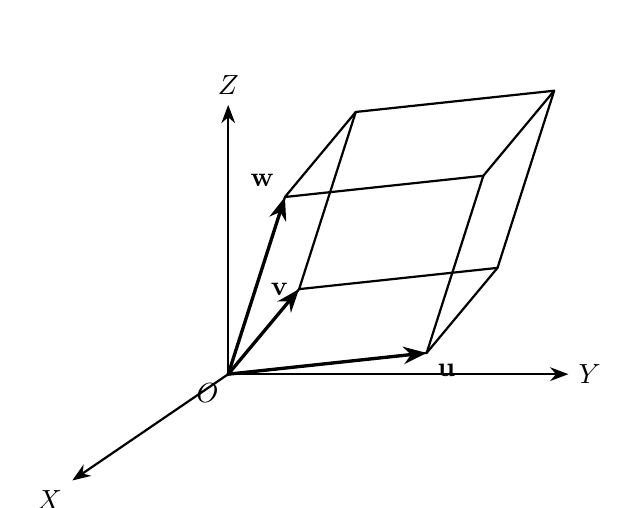
\begin{tikzpicture}[>=Stealth, scale=0.9, line cap=round, line join=round]
  % Axes
  \draw[->, thick] (0, 0) -- (-2.2, -1.5) node[below left] {$X$};
  \draw[->, thick] (0, 0) -- (4.8, 0) node[right] {$Y$};
  \draw[->, thick] (0, 0) -- (0, 3.8) node[above] {$Z$};
  \node[below left] at (0,0) {$O$};

  % Vectors u, v, w
  % Let u = (-2, 5, 1) -> visual coords: u_x = -0.7*(-2) + 0.8*(5) etc.
  % We project (x,y,z) to (y - 0.7*x, z - 0.5*x)
  % For visual clarity, choose attractive 3d oblique projection:
  \coordinate (O) at (0,0);
  \coordinate (U) at (2.8, 0.3); % vector u
  \coordinate (V) at (1.0, 1.2); % vector v
  \coordinate (W) at (0.8, 2.5); % vector w

  \coordinate (UV) at ($(U)+(V)$);
  \coordinate (UW) at ($(U)+(W)$);
  \coordinate (VW) at ($(V)+(W)$);
  \coordinate (UVW) at ($(U)+(V)+(W)$);

  % Draw base
  \draw[thick] (O) -- (U);
  \draw[thick] (O) -- (V);
  \draw[thick] (U) -- (UV);
  \draw[thick] (V) -- (UV);

  % Draw vertical edges
  \draw[thick] (O) -- (W);
  \draw[thick] (U) -- (UW);
  \draw[thick] (V) -- (VW);
  \draw[thick] (UV) -- (UVW);

  % Draw top face
  \draw[thick] (W) -- (UW) -- (UVW) -- (VW) -- cycle;

  % Arrows for u, v, w
  \draw[->, very thick] (O) -- (U) node[below right] {$\vect{u}$};
  \draw[->, very thick] (O) -- (V) node[left] {$\vect{v}$};
  \draw[->, very thick] (O) -- (W) node[above left] {$\vect{w}$};
\end{tikzpicture}
\caption*{圖 2-1}\label{fig:b6-2-1}
\end{figure}

今考慮一個二階方陣，分別以 $\vect{a}_1=(a_{11}, a_{12}), \vect{a}_2=(a_{21}, a_{22})$ 表其第一、第二列向量，此方陣可記為 $\begin{bmatrix} \vect{a}_1 \\ \vect{a}_2 \end{bmatrix}$。我們來複習一下第三冊 § 3-7 中的演算，以決定由 $\vect{a}_1, \vect{a}_2$ 所張出的平行四邊形的面積 $V$。取 $\vect{u} = \dfrac{\vect{a}_1}{|\vect{a}_1|}$ 為 $\vect{a}_1$ 的方向，則顯然如圖 2-2 所示：

\begin{figure}[H]
\centering
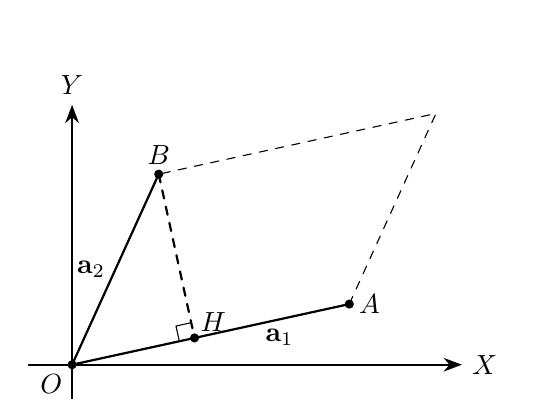
\begin{tikzpicture}[>=Stealth, scale=1.1, line cap=round, line join=round]
  \draw[->, thick] (-0.5, 0) -- (4.5, 0) node[right] {$X$};
  \draw[->, thick] (0, -0.5) -- (0, 3.0) node[above] {$Y$};
  \node[below left] at (0,0) {$O$};

  \coordinate (O) at (0,0);
  \coordinate (A) at (3.2, 0.7);
  \coordinate (B) at (1.0, 2.2);
  \coordinate (D) at ($(A)+(B)$);
  % Orthogonal projection of B onto line OA
  \coordinate (H) at ($(O)!(B)!(A)$);

  \draw[thick] (O) -- (A);
  \node[below] at ($(H)!0.55!(A)$) {$\vect{a}_1$};
  \draw[thick] (O) -- (B) node[midway, left] {$\vect{a}_2$};
  \draw[dashed] (A) -- (D) -- (B);
  \draw[dashed, thick] (B) -- (H);

  \fill (O) circle (1.5pt);
  \fill (A) circle (1.5pt) node[right] {$A$};
  \fill (B) circle (1.5pt) node[above] {$B$};
  \fill (H) circle (1.5pt) node[above right, inner sep=2pt] {$H$};

  % Right angle mark at H
  \draw ($(H)!0.18cm!(B)$) -- ($($(H)!0.18cm!(B)$)+($(H)!0.18cm!(O)$)-(H)$) -- ($(H)!0.18cm!(O)$);
\end{tikzpicture}
\caption*{圖 2-2}\label{fig:b6-2-2}
\end{figure}

\begin{equation}
V = \overline{OA} \cdot \overline{HB} = |\vect{a}_1| \cdot |\vect{a}_2 - (\vect{a}_2 \cdot \vect{u})\vect{u}| \label{eq:b6-1-2-3}
\end{equation}
由第三冊 § 3-7 的計算得
\[ V = |a_{11} a_{22} - a_{12} a_{21}| = \left| \begin{vmatrix} a_{11} & a_{12} \\ a_{21} & a_{22} \end{vmatrix} \right| \text{ 的絕對值} \]
即方陣 $\begin{bmatrix} \vect{a}_1 \\ \vect{a}_2 \end{bmatrix}$ 的行列式的絕對值。我們曾以 $|\vect{a}_1 \wedge \vect{a}_2|$ 表示。為了討論方便，有時用 $\det \begin{bmatrix} \vect{a}_1 \\ \vect{a}_2 \end{bmatrix}$ 或 $|a_{ij}|$ 表 $\begin{vmatrix} a_{11} & a_{12} \\ a_{21} & a_{22} \end{vmatrix}$。若是除去絕對值的符號，$\det \begin{bmatrix} \vect{a}_1 \\ \vect{a}_2 \end{bmatrix}$ 所代表的就是稱作\textbf{有向面積}，記作 $V(\vect{a}_1, \vect{a}_2)$。顯然，$V(\vect{a}_2, \vect{a}_1) = -V(\vect{a}_1, \vect{a}_2)$ 此式表明 $V(\vect{a}_1, \vect{a}_2)$ 的值因向量選取的次序而易號。當然，負面積原是沒有意義的，這樣的安排是為著方向的考慮和討論的方便。

三維空間中平行六面體的體積又如何求法？（請參閱第三冊 § 3-7，又見同冊第五章作業 8 和習題 5-2 我們把這問題重作詳述。）設 $\vect{a}_1=(a_{11}, a_{12}, a_{13}), \vect{a}_2=(a_{21}, a_{22}, a_{23}), \vect{a}_3=(a_{31}, a_{32}, a_{33})$ 為 $\mathbb{R}^3$ 中三向量，今考慮三者所張出平行六面體：如圖 2-3，自 $O$ 分別取向量 $\vect{a}_1, \vect{a}_2, \vect{a}_3$，先計算由 $\vect{a}_1, \vect{a}_2$ 所張出 $\square OADB$ 的面積，再乘以高度 $\overline{CE}$ 便得到所求平行六面體的體積了。今仿上段求法，計算 $\square OADB$ 面積如下（見圖 2-3）：

取 $\vect{u}=\dfrac{\vect{a}_1}{|\vect{a}_1|}$\phantomsection\label{note:b6-ch1-p24-u}\footnote{【原書校訂】：原書此處印作「$\vect{u}=\frac{\vect{a}}{|\vect{a}|}$」，漏下標 $1$，據上下文校訂為「$\vect{u}=\frac{\vect{a}_1}{|\vect{a}_1|}$」。}，則

$\vect{a}_2$ 在 $\vect{u}$ 方向的投影
\[ \vec{OH} = (\vect{a}_2 \cdot \vect{u})\vect{u} \]
故
\[ \vec{HB} = \vec{OB} - \vec{OH} = \vect{a}_2 - (\vect{a}_2 \cdot \vect{u})\vect{u} \]
\begin{align*}
(\square OADB \text{ 的面積})^2 &= |\vect{a}_2 - (\vect{a}_2 \cdot \vect{u})\vect{u}|^2 |\vect{a}_1|^2 \\
&= \left[ |\vect{a}_2|^2 - \left(\dfrac{\vect{a}_2 \cdot \vect{a}_1}{|\vect{a}_1|}\right)^2 \right] |\vect{a}_1|^2 \\
&= |\vect{a}_1|^2 |\vect{a}_2|^2 - (\vect{a}_1 \cdot \vect{a}_2)^2
\end{align*}
設 $\vect{v} = \dfrac{\vect{a}_2 - (\vect{a}_2 \cdot \vect{u})\vect{u}}{|\vect{a}_2 - (\vect{a}_2 \cdot \vect{u})\vect{u}|}$ 為 $\vec{HB}$ 的方向（單位向量），則向量 $\vec{OC}$ 在 $\square OADB$ 上的投影 $\vec{OE}$ 可表為
\[ \vec{OE} = (\vect{a}_3 \cdot \vect{u})\vect{u} + (\vect{a}_3 \cdot \vect{v})\vect{v} \]
且
\[ \vec{EC} = \vect{a}_3 - (\vect{a}_3 \cdot \vect{u})\vect{u} - (\vect{a}_3 \cdot \vect{v})\vect{v}\footnotemark \]
\footnotetext{【原書註】：因為 $\vec{EC}\cdot\vect{u} = \vec{EC}\cdot\vect{v} = 0$，故在 $\vec{EC}$ 與平面上任一向量均垂直，即 $\vec{EC} \perp \text{平面 } OADB$。又 $\vect{a}_3 \cdot \vec{EC} = |\vect{a}_3|^2 - (\vect{a}_3\cdot\vect{u})^2 - (\vect{a}_3\cdot\vect{v})^2 = \vec{EC}\cdot\vec{EC} = |\vec{EC}|^2 > 0$，又且 $\vect{a}_3 \cdot \vec{EC} = |\vect{a}_3|\,|\vec{EC}|\cos\theta$（$\theta$ 為二向量交角），即 $|\vec{EC}| = |\vect{a}_3|\cos\theta$，表示 $\vec{EC} \perp \vec{OE}$（因 $\vec{EC}$ 為 $\vect{a}_3$ 在直線 $EC$ 上的投影）。又 $0 \le \theta \le \frac{\pi}{2}$，所以 $\vec{EC}=\vect{a}_3$ 在直線 $EC$ 上的投影。（$0 \le \theta \le \frac{\pi}{2}$ 除去了“$-\vec{EC}=\vect{a}_3$ 在直線 $EC$ 上的投影”這一可能性）}

\begin{figure}[H]
\centering
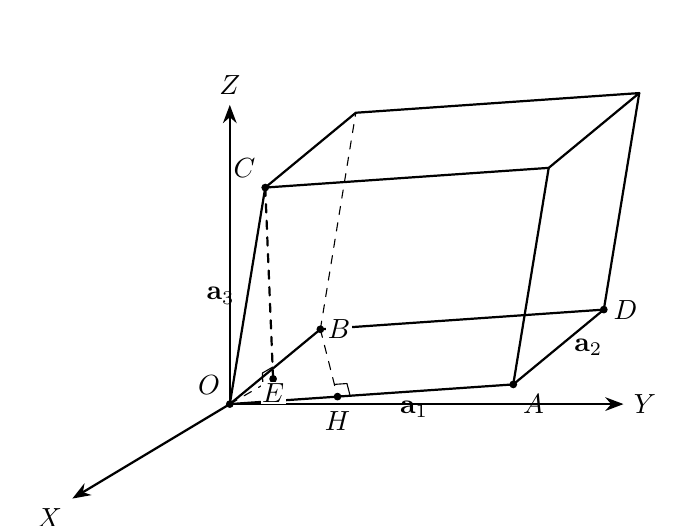
\begin{tikzpicture}[>=Stealth, scale=1.0, line cap=round, line join=round]
  % Axes
  \draw[->, thick] (0, 0) -- (-2.0, -1.2) node[below left] {$X$};
  \draw[->, thick] (0, 0) -- (5.0, 0) node[right] {$Y$};
  \draw[->, thick] (0, 0) -- (0, 3.8) node[above] {$Z$};
  \node[above left] at (0,0) {$O$};

  \coordinate (O) at (0,0);
  \coordinate (A) at (3.6, 0.25); % a1
  \coordinate (B) at (1.15, 0.95); % a2
  \coordinate (D) at ($(A)+(B)$);
  \coordinate (C) at (0.45, 2.75); % a3

  \coordinate (Ap) at ($(A)+(C)$);
  \coordinate (Bp) at ($(B)+(C)$);
  \coordinate (Dp) at ($(D)+(C)$);

  % Base parallelogram
  \draw[thick] (O) -- (A);
  \node[below] at ($(O)!0.65!(A)$) {$\vect{a}_1$};
  \draw[thick] (O) -- (B);
  \draw[thick] (A) -- (D) node[midway, right=2pt] {$\vect{a}_2$};
  \draw[thick] (B) -- (D);

  % Top parallelogram
  \draw[thick] (C) -- (Ap) -- (Dp) -- (Bp) -- cycle;

  % Vertical edges
  \draw[thick] (O) -- (C) node[midway, left=1pt] {$\vect{a}_3$};
  \draw[thick] (A) -- (Ap);
  \draw[dashed] (B) -- (Bp);
  \draw[thick] (D) -- (Dp);

  % Points H (foot of B on OA) and E (foot of C on base plane)
  \path (O) -- (A) coordinate[pos=0.38] (H);
  \coordinate (E) at (0.55, 0.32);

  \draw[dashed] (B) -- (H);
  \draw[dashed, thick] (C) -- (E);
  \draw[dashed] (O) -- (E);

  % Right-angle mark at H (HB perp OA)
  \draw ($(H)!0.16cm!(B)$) -- ($($(H)!0.16cm!(B)$)+($(H)!0.16cm!(A)$)-(H)$) -- ($(H)!0.16cm!(A)$);
  % Right-angle mark at E (CE perp OE)
  \draw ($(E)!0.15cm!(C)$) -- ($($(E)!0.15cm!(C)$)+($(E)!0.15cm!(O)$)-(E)$) -- ($(E)!0.15cm!(O)$);

  \fill (O) circle (1.4pt);
  \fill (A) circle (1.4pt) node[below right] {$A$};
  \fill (B) circle (1.4pt) node[right=2pt, fill=white, inner sep=0.5pt] {$B$};
  \fill (D) circle (1.4pt) node[right] {$D$};
  \fill (C) circle (1.4pt) node[above left] {$C$};
  \fill (H) circle (1.4pt) node[below=2pt] {$H$};
  \fill (E) circle (1.4pt) node[right=2pt, below=1pt, fill=white, inner sep=0.5pt] {$E$};
\end{tikzpicture}
\caption*{圖 2-3}\label{fig:b6-2-3}
\end{figure}

所求平行六面體的體積 $V$ 可以計算如下：
\begin{align*}
V^2 &= \left[ |\vect{a}_1|^2 |\vect{a}_2|^2 - (\vect{a}_1 \cdot \vect{a}_2)^2 \right] |\vect{a}_3 - (\vect{a}_3 \cdot \vect{u})\vect{u} - (\vect{a}_3 \cdot \vect{v})\vect{v}|^2 \\
&= \left[ |\vect{a}_1|^2 |\vect{a}_2|^2 - (\vect{a}_1 \cdot \vect{a}_2)^2 \right] \left[ |\vect{a}_3|^2 - (\vect{a}_3 \cdot \vect{u})^2 - (\vect{a}_3 \cdot \vect{v})^2 \right] \\
&= \left[ |\vect{a}_1|^2 |\vect{a}_2|^2 - (\vect{a}_1 \cdot \vect{a}_2)^2 \right] \left[ |\vect{a}_3|^2 - \dfrac{(\vect{a}_3 \cdot \vect{a}_1)^2}{|\vect{a}_1|^2} - \dfrac{((\vect{a}_3 \cdot \vect{a}_2) - (\vect{a}_2 \cdot \vect{u})(\vect{a}_3 \cdot \vect{u}))^2 |\vect{a}_1|^2}{|\vect{a}_1|^2 |\vect{a}_2|^2 - (\vect{a}_1 \cdot \vect{a}_2)^2} \right] \\
&= |\vect{a}_1|^2 \cdot |\vect{a}_2|^2 \cdot |\vect{a}_3|^2 - (\vect{a}_1 \cdot \vect{a}_2)^2 |\vect{a}_3|^2 - (\vect{a}_3 \cdot \vect{a}_1)^2 |\vect{a}_2|^2 \\
&\quad - (\vect{a}_3 \cdot \vect{a}_2)^2 |\vect{a}_1|^2 + 2(\vect{a}_1 \cdot \vect{a}_3)(\vect{a}_3 \cdot \vect{a}_2)(\vect{a}_2 \cdot \vect{a}_1) \\
&= (a_{11}^2 + a_{12}^2 + a_{13}^2)(a_{21}^2 + a_{22}^2 + a_{23}^2)(a_{31}^2 + a_{32}^2 + a_{33}^2) \\
&\quad - (a_{11}a_{21} + a_{12}a_{22} + a_{13}a_{23})^2 (a_{31}^2 + a_{32}^2 + a_{33}^2) \\
&\quad - (a_{11}a_{31} + a_{12}a_{32} + a_{13}a_{33})^2 (a_{21}^2 + a_{22}^2 + a_{23}^2) \\
&\quad - (a_{21}a_{31} + a_{22}a_{32} + a_{23}a_{33})^2 (a_{11}^2 + a_{12}^2 + a_{13}^2) \\
&\quad + 2(a_{21}a_{31} + a_{22}a_{32} + a_{23}a_{33})(a_{11}a_{21} + a_{12}a_{22} + a_{13}a_{23})(a_{11}a_{31} + a_{12}a_{32} + a_{13}a_{33}) \\
&= (a_{11}a_{22}a_{33} + a_{13}a_{21}a_{32} + a_{12}a_{23}a_{31} - a_{13}a_{22}a_{31} - a_{12}a_{21}a_{33} - a_{11}a_{23}a_{32})^2 \\
&= \begin{vmatrix}
a_{11} & a_{12} & a_{13} \\
a_{21} & a_{22} & a_{23} \\
a_{31} & a_{32} & a_{33}
\end{vmatrix}^2
\end{align*}
\[ V = \left| \det \begin{bmatrix} \vect{a}_1 \\ \vect{a}_2 \\ \vect{a}_3 \end{bmatrix} \right| \]
若去掉絕對值的符號，$\det \begin{bmatrix} \vect{a}_1 \\ \vect{a}_2 \\ \vect{a}_3 \end{bmatrix}$ 所代表的就是稱作此平行六面體的\textbf{有向體積}，記作 $V(\vect{a}_1, \vect{a}_2, \vect{a}_3)$。變換 $\vect{a}_1, \vect{a}_2, \vect{a}_3$ 中任兩列向量的次序，則相差一負號。例如 $V(\vect{a}_3, \vect{a}_2, \vect{a}_1) = -V(\vect{a}_1, \vect{a}_2, \vect{a}_3)$。這三向量 $\vect{a}_1, \vect{a}_2, \vect{a}_3$ 選取的次序與物理上所指左手定則或右手定則有關，作為定向之用，也是 $\det \begin{bmatrix} \vect{a}_1 \\ \vect{a}_2 \\ \vect{a}_3 \end{bmatrix}$ 值為正或為負的來源，在這裏就不細述了。

雖然上述這種求體積的方法已經比從純粹座標幾何的角度來處理要精簡得多，可仍然是十分繁瑣。在求一般 $\mathbb{R}^n$ 中 $n$ 維平行體的“體積”時（確切地說，推廣 $\mathbb{R}^3$ 中平行六面體的體積算法——底部平行四邊形的面積乘以高度——到一般 $\mathbb{R}^n$ 的情形時）這樣的計算顯然不是一個理想的方法。

我們嚐試列舉並分析一下 $\mathbb{R}^2$ 中的平行四邊形有向面積與 $\mathbb{R}^3$ 中平行六面體有向體積的一些基本性質，希望能抽出一些作為行列式的定義，用以求取一般 $\mathbb{R}^n$ 中 $n$ 維平行體的體積。

令 $\vect{a}, \vect{b}, \vect{c}$ 為 $\mathbb{R}^2$ 中三向量，以 $V(\vect{a}, \vect{b})$ 表 $\vect{a}, \vect{b}$ 所張平行四邊形之有向面積（亦即容許有負值的面積）。下面幾個性質可以從圖上清楚看出：
\begin{enumerate}[label=\Roman*., leftmargin=2.5em]
  \item $V(\lambda\vect{a}, \vect{b}) = \lambda V(\vect{a}, \vect{b})$ 對任意實數 $\lambda$ 均滿足。見圖 2-4。
  
  \begin{figure}[H]
  \centering
  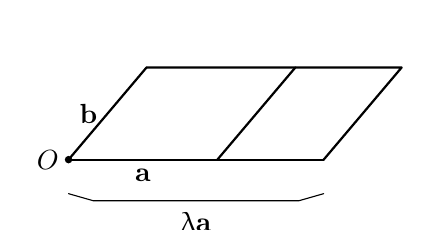
\begin{tikzpicture}[>=Stealth, scale=0.9, line cap=round, line join=round]
    \coordinate (O) at (0,0);
    \coordinate (A) at (2.1, 0);
    \coordinate (B) at (1.1, 1.3);
    \coordinate (AB) at ($(A)+(B)$);
    \coordinate (lA) at (3.6, 0);
    \coordinate (lAB) at ($(lA)+(B)$);

    \draw[thick] (O) -- (lA);
    \draw[thick] (O) -- (B) node[midway, left] {$\vect{b}$};
    \draw[thick] (B) -- (lAB) -- (lA);
    \draw[thick] (AB) -- (A);
    \node[below] at ($(O)!0.5!(A)$) {$\vect{a}$};

    % Bracket/span for \lambda a
    \draw[thin] (0,-0.48) -- (0.35,-0.58) -- (3.25,-0.58) -- (3.6,-0.48);
    \node[below] at (1.8, -0.60) {$\lambda\vect{a}$};

    \fill (O) circle (1.5pt) node[left] {$O$};
  \end{tikzpicture}
  \caption*{圖 2-4}\label{fig:b6-2-4}
  \end{figure}

  \item $V(\vect{a}+\vect{c}, \vect{b}) = V(\vect{a}, \vect{b}) + V(\vect{c}, \vect{b})$\\
  如圖 2-5 所示 $\triangle OQT \cong \triangle SRU$\\
  所以
  \begin{align*}
  \square OTUS \text{ 的面積} &= \square OQRS \text{ 的面積} + \square QTUR \text{ 的面積}
  \end{align*}
  同理 $V(\vect{a}, \vect{b}+\vect{c}) = V(\vect{a}, \vect{b}) + V(\vect{a}, \vect{c})$。

  \begin{figure}[H]
  \centering
  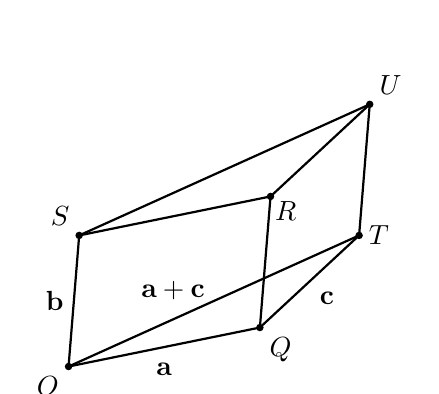
\begin{tikzpicture}[>=Stealth, scale=0.9, line cap=round, line join=round]
    \coordinate (O) at (0,0);
    \coordinate (Q) at (2.7, 0.55);
    \coordinate (T) at (4.1, 1.85);
    \coordinate (S) at (0.15, 1.85);
    \coordinate (R) at ($(Q)+(S)$);
    \coordinate (U) at ($(T)+(S)$);

    \draw[thick] (O) -- (Q) node[midway, below=2pt] {$\vect{a}$};
    \draw[thick] (Q) -- (T) node[midway, below right] {$\vect{c}$};
    \draw[thick] (O) -- (S) node[midway, left] {$\vect{b}$};
    \draw[thick] (S) -- (R) -- (U);
    \draw[thick] (Q) -- (R);
    \draw[thick] (T) -- (U);
    \draw[thick] (O) -- (T);
    \node[above left, inner sep=1pt] at ($(O)!0.48!(T)$) {$\vect{a}+\vect{c}$};
    \draw[thick] (S) -- (U);

    \fill (O) circle (1.5pt) node[below left] {$O$};
    \fill (Q) circle (1.5pt) node[below right] {$Q$};
    \fill (T) circle (1.5pt) node[right] {$T$};
    \fill (S) circle (1.5pt) node[above left] {$S$};
    \fill (R) circle (1.5pt) node[below right, inner sep=1.5pt] {$R$};
    \fill (U) circle (1.5pt) node[above right] {$U$};
  \end{tikzpicture}
  \caption*{圖 2-5}\label{fig:b6-2-5}
  \end{figure}

  \item $V(\vect{a}, \vect{b}+\lambda\vect{a}) = V(\vect{a}, \vect{b})$\\
  如圖 2-6，同底等高的平行四邊形面積相同。同理 $V(\vect{a}+\lambda\vect{b}, \vect{b}) = V(\vect{a}, \vect{b})$。

  \begin{figure}[H]
  \centering
  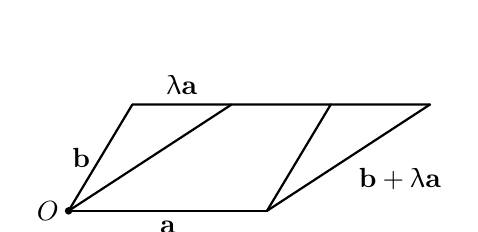
\begin{tikzpicture}[>=Stealth, scale=0.9, line cap=round, line join=round]
    \coordinate (O) at (0,0);
    \coordinate (A) at (2.8, 0);
    \coordinate (B) at (0.9, 1.5);
    \coordinate (AB) at ($(A)+(B)$);
    \coordinate (Bp) at ($(B)+(1.4, 0)$);
    \coordinate (ABp) at ($(AB)+(1.4, 0)$);

    \draw[thick] (O) -- (A) node[midway, below] {$\vect{a}$};
    \draw[thick] (O) -- (B) node[midway, left] {$\vect{b}$};
    \draw[thick] (B) -- (AB) -- (A);

    \draw[thick] (O) -- (Bp);
    \draw[thick] (A) -- (ABp) node[midway, below right] {$\vect{b}+\lambda\vect{a}$};
    \draw[thick] (AB) -- (ABp);
    \node[above] at ($(B)!0.5!(Bp)$) {$\lambda\vect{a}$};

    \fill (O) circle (1.5pt) node[left] {$O$};
  \end{tikzpicture}
  \caption*{圖 2-6}\label{fig:b6-2-6}
  \end{figure}

  \item $V(\vect{a}, \vect{a}) = 0$\\
  因為在平面上，一線段的面積為 0。

  \item $\vect{e}_1=(1, 0), \vect{e}_2=(0, 1)$，則
  \[ V(\vect{e}_1, \vect{e}_2) = 1 \]
  因邊長為 1 的正方形其面積為 1。
\end{enumerate}

\subsubsection*{作業 18}\label{hw:b6-1-18}
\begin{enumerate}[label=(\roman*), leftmargin=2em]
  \item 以上從 I 到 V 的性質，對 $\mathbb{R}^3$ 中平行六面體亦相應成立，試將其相應性質用式子列出。
  \item $\mathbb{R}^1$ 中又當如何去敘述？
\end{enumerate}

以上性質事實上有些可以從另一些導出，是彼此相關的。我們將抽出其中幾個，將之推廣到一般 $\mathbb{R}^n$ 中。

\begin{definition}\label{def:b6-1-5}
設 $V$ 為 $\mathbb{R}^n$ 中自 $n$ 個向量 $\vect{a}_1, \vect{a}_2, \dots, \vect{a}_n$ 映至 $\mathbb{R}$ 的函數，記作 $V(\vect{a}_1, \vect{a}_2, \dots, \vect{a}_n)$ 滿足下列四個性質：
\begin{enumerate}[label=(\Alph*), leftmargin=2em]
  \item $V(\vect{a}_1, \dots, \vect{a}_i, \dots, \vect{a}_n) = V(\vect{a}_1, \dots, \vect{a}_i + \vect{a}_k, \dots, \vect{a}_n); \quad i \ne k, 1 \le i \le n, 1 \le k \le n$
  \item $V(\vect{a}_1, \dots, \lambda\vect{a}_i, \dots, \vect{a}_n) = \lambda V(\vect{a}_1, \dots, \vect{a}_i, \dots, \vect{a}_n) \qquad 1 \le i \le n$
  \item $V(\vect{b} + \vect{c}, \vect{a}_2, \dots, \vect{a}_n) = V(\vect{b}, \vect{a}_2, \dots, \vect{a}_n) + V(\vect{c}, \vect{a}_2, \dots, \vect{a}_n)$
  \item $V(\vect{e}_1, \vect{e}_2, \dots, \vect{e}_n) = 1$
\end{enumerate}
此函數 $V$ 稱為\textbf{行列式}（或 \textbf{$n$ 階行列式}）。
\end{definition}

亦可以把 $V$ 看作是 $\mathbb{R}^{n^2}$ 到 $\mathbb{R}$ 的函數。又若把 $\vect{a}_i$ 看作列向量，我們可以把 $V$ 看作將 $n$ 階方陣映至 $\mathbb{R}$ 的函數，常記作
\begin{equation}
V(\vect{a}_1, \vect{a}_2, \dots, \vect{a}_n) = \begin{vmatrix}
a_{11} & a_{12} & \dots & a_{1n} \\
a_{21} & a_{22} & \dots & a_{2n} \\
\dots & \dots & \dots & \dots \\
a_{n1} & a_{n2} & \dots & a_{nn}
\end{vmatrix} \label{eq:b6-1-2-4}
\end{equation}
\begin{equation}
\text{或簡記作 } |a_{ij}|\text{。} \tag{4'} \label{eq:b6-1-2-4p}
\end{equation}

其中 $\vect{a}_i=(a_{i1}, a_{i2}, \dots, a_{in})$ 為列向量，$i=1, 2, \dots, n$。
所以我們仍稱 $a_{ij}$ 為第 $i$ 列第 $j$ 行的原素，$\vect{a}_j^*=(a_{1j}, a_{2j}, \dots, a_{nj})$ 為行向量。事實上我們將要看到方陣的運算與行列式的運算間有密切的關係。

現在我們面臨三個重要問題：
\begin{enumerate}[label=(\roman*), leftmargin=2em]
  \item 這種行列式函數是否存在？
  \item 若是存在，是否僅有一個這樣的函數？（此即唯一性）
  \item 假設存在而且唯一，我們又如何去計算 $V(\vect{a}_1, \vect{a}_2, \dots, \vect{a}_n)$ 呢？
\end{enumerate}

\paragraph{注意：}(C) 稱作行列式加法定理，事實上可由 (A), (B) 兩式證得（參閱附錄 II）。為了簡化討論和集中注意，我們在課文內將不深究。

由上面的討論可以理解，若對 (i), (ii) 的答案均是肯定的，我們可以用行列式來定義 $n$ 維平行體的“有向體積”，因為此時滿足這些性質的函數為唯一存在。

\subsubsection*{習題 I-2}\label{sec:b6-ex1-2}

\begin{enumerate}[label=\arabic*., leftmargin=2em]
  \item 當 $\vect{a}_1, \vect{a}_2$ 為下列各種情形時，試求 $V(\vect{a}_1, \vect{a}_2)$ 並作圖：
  \begin{enumerate}[label=(\roman*)]
    \item $\vect{a}_1=(1, 2), \vect{a}_2=(3, -1)$
    \item $\vect{a}_1=(-1, 3), \vect{a}_2=(-2, 0)$
  \end{enumerate}

  \item 當 $\vect{a}_1, \vect{a}_2, \vect{a}_3$ 為下列各種情形時，試求 $V(\vect{a}_1, \vect{a}_2, \vect{a}_3)$ 並作圖：
  \begin{enumerate}[label=(\roman*)]
    \item $\vect{a}_1=(1, 0, 1), \vect{a}_2=(0, 1, 1), \vect{a}_3=(1, 1, 0)$
    \item $\vect{a}_1=(1, -1, 2), \vect{a}_2=(-1, 0, 3), \vect{a}_3=(0, 2, -1)$
  \end{enumerate}

  \item $P=(1, -2, 1), Q=(2, 0, 2), R=(5, 6, 3)$ 試求 $\triangle PQR$ 的面積。

  \stepcounter{enumi}
  \item[\textbf{*4.}] 設 $U$ 為 $\mathbb{R}^n$ 中任何 $n$ 個向量 $\vect{a}_1, \vect{a}_2, \dots, \vect{a}_n$ 映到 $\mathbb{R}$ 的一個函數，記作 $U(\vect{a}_1, \vect{a}_2, \dots, \vect{a}_n)$ 且滿足 (A), (B), (C) 三性質。若 $k$ 為一實數，令
  \[ W(\vect{a}_1, \vect{a}_2, \dots, \vect{a}_n) = k U(\vect{a}_1, \vect{a}_2, \dots, \vect{a}_n) \]
  則是否 $W$ 也滿足 (A), (B), (C) 三性質？

  \stepcounter{enumi}
  \item[\textbf{*5.}] $\mathbb{R}^3$ 中由不共面的四點 $P, Q, R, S$ 為頂點所張成的凸面體稱為四面體，即
  \[ \text{四面體} = \{ \vec{OT} : \vec{OT} = \lambda_1\vec{OP} + \lambda_2\vec{OQ} + \lambda_3\vec{OR} + \lambda_4\vec{OS}, \lambda_1+\lambda_2+\lambda_3+\lambda_4 = 1 \} \]
  若已知四面體的體積為 $P, Q, R, S$ 所張成平行六面體體積的六分之一。試求下列各四點所成四面體的體積：
  \begin{enumerate}[label=(\roman*)]
    \item $(0, 0, 0), (1, 0, 0), (0, 1, 0), (0, 2, 3)$
    \item $(0, 1, 2), (3, 1, 4), (1, 2, 3), (4, 1, 0)$
  \end{enumerate}

  \item 設 $P, Q, R, S \in \mathbb{R}^3$，試求在下面情形時，四面體的面積，若所得面積為零時，則 $P, Q, R, S$ 之關係為何？
  \phantomsection\label{note:b6-ch1-p30-s-coord}%
  \[ P=(1, 1, 0), Q=(0, -1, 1), R=(-4, 1, -5), S=(0, 0, 0)\footnotemark \]
  \footnotetext{【原書校訂】：原書此處印作「$S=(0,0,0($」，右括弧印損，茲校訂補正為「$S=(0,0,0)$」。}

  \item 設 $\vect{a}_1=(a_{11}, a_{12}, a_{13}), \vect{a}_2=(a_{21}, a_{22}, a_{23})$ 為 $\mathbb{R}^3$ 中二向量，試證 $\vect{a}_1, \vect{a}_2$ 所張平行四邊形的面積為
  \[ \sqrt{\begin{vmatrix} a_{12} & a_{13} \\ a_{22} & a_{23} \end{vmatrix}^2 + \begin{vmatrix} a_{13} & a_{11} \\ a_{23} & a_{21} \end{vmatrix}^2 + \begin{vmatrix} a_{11} & a_{12} \\ a_{21} & a_{22} \end{vmatrix}^2} \]
\end{enumerate}

\subsection{重排與符號函數}\label{sec:b6-1-3}
\resetsectcounters

\paragraph{觀察：}
\begin{equation}
\begin{vmatrix}
a_1 & a_2 & a_3 \\
b_1 & b_2 & b_3 \\
c_1 & c_2 & c_3
\end{vmatrix} = a_1 b_2 c_3 + a_3 b_1 c_2 + a_2 b_3 c_1 - a_3 b_2 c_1 - a_2 b_1 c_3 - a_1 b_3 c_2 \label{eq:b6-1-3-1}
\end{equation}
我們發現三件事：
\begin{enumerate}[label=\arabic*., leftmargin=2em]
  \item 右邊的每一項 $a_i b_j c_k$ 其中 $i, j, k$ 均相異，這表明此項是由每一行每一列均只取一個原素相乘而得。
  \item 每一項 $a_i b_j c_k$ 中 $a, b, c$ 三英文字母均不同，因此可把 $a_i b_j c_k$ 與 $1, 2, 3$ 的排列作一對應，此對應顯然成一個一一對應即右邊恰有 $3!$ 項。
  \item 右邊有些項取正號，有些項取負號，這符號規則為何？又若是推廣到一般 $n$ 階情形，其符號規定有沒有一定的法則可尋？
\end{enumerate}

設 $N(n) = \{ 1, 2, \dots, n \}$，今考慮一個從 $N(n)$ 映成到 $N(n)$ 的函數 $\pi$，顯然 $\pi$ 必為一個單射。將 $\pi(1), \pi(2), \dots, \pi(n)$ 按序寫出，可看出 $\pi$ 等於是自 1 到 $n$ 這 $n$ 個正整數的一種排列。反之，任何一個這樣的排列都可以看成為自 $N(n)$ 映成到 $N(n)$ 的函數。我們有時將 $\pi$ 記為
\begin{equation}
\pi : \begin{pmatrix} 1 & 2 & \dots & n \\ \pi(1) & \pi(2) & \dots & \pi(n) \end{pmatrix} \label{eq:b6-1-3-2}
\end{equation}
或簡寫為
\begin{equation}
(\pi(1) \, \pi(2) \, \dots \, \pi(n)) \tag{2'} \label{eq:b6-1-3-2p}
\end{equation}

\begin{example}\label{ex:b6-1-12}
設 $\pi: N(5) \longrightarrow N(5)$ 定義如下：
\[ \pi : \begin{pmatrix} 1 & 2 & 3 & 4 & 5 \\ \pi(1) & \pi(2) & \pi(3) & \pi(4) & \pi(5) \end{pmatrix} \]
$\pi(1)=3, \pi(2)=5, \pi(3)=4, \pi(4)=1, \pi(5)=2$。
若寫作 $(3 \; 5 \; 4 \; 1 \; 2)$ 就更清楚看出 $\pi$ 代表一種 $N(5)$ 的排列。\hfill$\#$
\end{example}

\begin{definition}\label{def:b6-1-6}
一個自 $N(n)$ 映成到 $N(n)$ 的函數 $\pi$ 稱作一個\textbf{重排}。
\end{definition}

在上例中有些數字的大小次序保持不變，有些卻更改了。例如 3 4 和 1 2 次序保持不變，可是 5 4 和 3 1 等次序卻改變了。在 $\pi$ 之下若有一對 $i, j, i < j$，使得 $\pi(i) > \pi(j)$，則稱重排 $\pi$ 有一個\textbf{倒置}。$\pi$ 中所有倒置的個數稱為\textbf{倒置數}，記為 $\#\pi$，或作 $\#(\pi(1)\pi(2)\dots\pi(n))$。

\begin{example}\label{ex:b6-1-13}
$\pi$ 如例 1，$\pi$ 的倒置數為何？
\end{example}

\paragraph{【解】}
$\pi$ 中所有倒置如下：$31, 32, 54, 51, 52, 41, 42$ 所以 $\#\pi = 7$。\hfill$\#$

關於倒置數，可看作將 $(\pi(1)\pi(2)\dots\pi(n))$ 的次序排回 $(1 \; 2 \; \dots \; n)$ 的次序所需經過對調兩數字的總次數。

\begin{example}\label{ex:b6-1-14}
$\pi$ 如例 2 表為 $(3 \; 5 \; 4 \; 1 \; 2)$，首先將 1 與 4 對調得 $(3 \; 5 \; 1 \; 4 \; 2)$，第二次將 1 與 5 對調得 $(3 \; 1 \; 5 \; 4 \; 2)$，第三次將 1 與 3 對調得 $(1 \; 3 \; 5 \; 4 \; 2)$，第四次將 2 與 5 對調得 $(1 \; 3 \; 2 \; 4 \; 5)$，第五次將 2 與 5 對調得 $(1 \; 3 \; 2 \; 5 \; 4)$，第六次將 2 與 3 對調得 $(1 \; 2 \; 3 \; 5 \; 4)$，第七次將 5 與 4 對調得 $(1 \; 2 \; 3 \; 4 \; 5)$。\hfill$\#$
\end{example}

\paragraph{注意：}我們也可以首先將 5 與 4 對調，其次將 1 與 5 對調等等。最後當我們比較兩次不同的過程，就會發現比如 5 與 1 的對調在兩次過程中出現的次序容或有不同，但卻相同的都出現一次。即所有的對調數並不因採行的過程不同而有所影響。

關於對調數還有一個實用之法來計算。今以前例作為說明。

\begin{discussion}\label{disc:b6-1-2}
$\pi$ 如前例，試求其倒置數。
\end{discussion}

\paragraph{【解】}
首先將 $\pi$ 如下寫出：
\[ \begin{matrix} 1 & 2 & 3 & 4 & 5 \\ 3 & 5 & 4 & 1 & 2 \end{matrix} \]

其次將表中上列與下列中相同的數字以直線相連，但要注意在劃線時不要讓三線以上有共點的情形發生：

\begin{figure}[H]
\centering
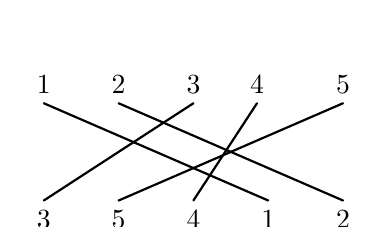
\begin{tikzpicture}[scale=0.95, line cap=round, line join=round]
  % Top row (slightly nudge 5 to avoid any triple intersection)
  \node (t1) at (1.0, 1.8) {$1$};
  \node (t2) at (2.0, 1.8) {$2$};
  \node (t3) at (3.0, 1.8) {$3$};
  \node (t4) at (3.85, 1.8) {$4$};
  \node (t5) at (5.0, 1.8) {$5$};
  % Bottom row
  \node (b3) at (1.0, 0) {$3$};
  \node (b5) at (2.0, 0) {$5$};
  \node (b4) at (3.0, 0) {$4$};
  \node (b1) at (4.0, 0) {$1$};
  \node (b2) at (5.0, 0) {$2$};
  % Connecting lines: 7 distinct pairwise intersections
  \draw[thick] (t1.south) -- (b1.north);
  \draw[thick] (t2.south) -- (b2.north);
  \draw[thick] (t3.south) -- (b3.north);
  \draw[thick] (t4.south) -- (b4.north);
  \draw[thick] (t5.south) -- (b5.north);
\end{tikzpicture}
\end{figure}

最後計算交點的個數正好是 7。現在來分析一下緣由：今以 1, 3 兩對數字所相應一對斜直線的交點為例，二斜直線所以會相交表明 1 3 在 $\pi$ 之下有了倒置，所以必相應一個對調。有 7 個交點表明有 7 個對調，所以倒置數為 7\footnote{\begin{minipage}[t]{0.95\linewidth}【原書註】：在計算符號函數時若有如下交點時：\par\smallskip
\centering
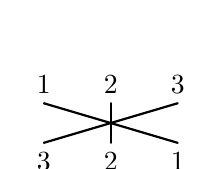
\begin{tikzpicture}[scale=0.85, line cap=round, line join=round]
  \node (u1) at (1, 1.15) {$1$}; \node (u2) at (2, 1.15) {$2$}; \node (u3) at (3, 1.15) {$3$};
  \node (d3) at (1, 0) {$3$}; \node (d2) at (2, 0) {$2$}; \node (d1) at (3, 0) {$1$};
  \draw[thick] (u1.south) -- (d1.north);
  \draw[thick] (u2.south) -- (d2.north);
  \draw[thick] (u3.south) -- (d3.north);
\end{tikzpicture}\par\smallskip
\raggedright 垂直線與斜線的交點可以不計。因垂直線與它線交點的總數必為偶數，不影響正負號。
\end{minipage}}。

下面的定義也是行列式展開式中的每一項其正負號的來源。

\begin{definition}\label{def:b6-1-7}
設 $F = \{ \pi : \pi \text{ 為 } N(n) \text{ 的重排} \}$（$F$ 共有 $n!$ 個元素），下面函數稱作\textbf{符號函數}，以 $\operatorname{sgn}$ 表示：
\[ \operatorname{sgn}(\pi) = \begin{cases}
1, & \#\pi \text{ 為偶數} \\
-1, & \#\pi \text{ 為奇數}
\end{cases} \]
通常 $\operatorname{sgn}(\pi)$ 亦可記為 $\operatorname{sgn}(\pi(1)\pi(2)\dots\pi(n))$。一般約定若 $\pi$ 不是映射，則定 $\operatorname{sgn}(\pi) = 0$。
\end{definition}

\subsubsection*{作業 19}\label{hw:b6-1-19}
試由上面定義中找到 (1) 式各項正負號的規則。

\subsubsection*{習題 I-3}\label{sec:b6-ex1-3}

\begin{enumerate}[label=\arabic*., leftmargin=2em]
  \item 設 $\pi$ 為下列各種情形時，試求 $\pi$ 的倒置數及 $\operatorname{sgn}(\pi)$：
  \begin{enumerate}[label=(\roman*)]
    \item $\pi = \begin{pmatrix} 1 & 2 & 3 & 4 & 5 \\ 2 & 3 & 4 & 5 & 1 \end{pmatrix}$
    \item $\pi = (3 \; 2 \; 4 \; 1 \; 6 \; 5)$
    \item $\pi = (7 \; 6 \; 5 \; 4 \; 3 \; 2 \; 1)$
  \end{enumerate}

  \stepcounter{enumi}
  \item[\textbf{*2.}] 設 $\pi \circ \pi^*$ 皆為 $N(n)$ 的重排
  \begin{enumerate}[label=(\roman*)]
    \item 試證合成函數 $\pi \circ \pi^*$ 也是 $N(n)$ 的一個重排。
    \item 試問 $\operatorname{sgn}(\pi \circ \pi^*)$ 與 $\operatorname{sgn}(\pi), \operatorname{sgn}(\pi^*)$ 之間的關係為何？
  \end{enumerate}

  \stepcounter{enumi}
  \item[\textbf{*3.}] 設 $i, j$ 為正整數，$1 \le i \le j \le n$，令
  \[ \pi_{ij} = \begin{pmatrix}
  1 & 2 & \dots & i-1 & i & i+1 & \dots & j-1 & j & j+1 & \dots & n \\
  1 & 2 & \dots & i-1 & j & i+1 & \dots & j-1 & i & j+1 & \dots & n
  \end{pmatrix} \]
  即將 $i, j$ 互調，其他數不動，試求 $\#\pi_{ij}$ 及 $\operatorname{sgn}(\pi_{ij})$。（提示：當 $n=4, 5$ 時，嚐試先作）

  \item 設 $\pi = (7 \; 6 \; 5 \; 4 \; 3 \; 2 \; 1)$。
  \begin{enumerate}[label=(\roman*)]
    \item 試證 $\pi = \pi_{17} \cdot \pi_{26} \cdot \pi_{35}$。
    \item 由習題 2, 3 試求 $\operatorname{sgn}(\pi)$ 之值。
  \end{enumerate}
\end{enumerate}

\subsection{行列式的基本性質}\label{sec:b6-1-4}
\resetsectcounters

在討論滿足 (A), (B), (C), (D) 的行列式函數是否存在以前，讓我們先從 (A), (B), (C), (D) 諸式推演行列式的若干性質：

\begin{theorem}\label{thm:b6-1-2}
$V(\vect{a}_1, \dots, \vect{a}_i, \dots, \vect{a}_n) = V(\vect{a}_1, \dots, \vect{a}_i + \lambda\vect{a}_k, \vect{a}_{i+1}, \dots, \vect{a}_n)$ 其中 $i \ne k$，$\lambda$ 為任意實數。亦即將 $\vect{a}_i$ 易為 $\vect{a}_i + \lambda\vect{a}_k$ 行列式的值不變。
\end{theorem}

\begin{proof}[【證明】]
$\lambda=0$ 時顯然成立。今假定 $\lambda \ne 0$，由 (B) 得
\[ V(\vect{a}_1, \dots, \lambda\vect{a}_k, \vect{a}_{k+1}, \dots, \vect{a}_n) = \lambda V(\vect{a}_1, \dots, \vect{a}_k, \vect{a}_{k+1}, \dots, \vect{a}_n) \]
又根據 (A)
\begin{align*}
V(\vect{a}_1, \dots, \vect{a}_i + \lambda\vect{a}_k, \dots, \lambda\vect{a}_k, \dots, \vect{a}_n) &= V(\vect{a}_1, \dots, \vect{a}_i, \dots, \lambda\vect{a}_k, \dots, \vect{a}_n) \\
&= \lambda V(\vect{a}_1, \dots, \vect{a}_i, \dots, \vect{a}_k, \dots, \vect{a}_n)
\end{align*}
（此處雖寫成 $i < k$ 的情形，其實對 $k < i$ 也是一樣的）\\
所以
\begin{align*}
\dfrac{1}{\lambda} V(\vect{a}_1, \dots, \vect{a}_i + \lambda\vect{a}_k, \dots, \lambda\vect{a}_k, \dots, \vect{a}_n) &= V(\vect{a}_1, \dots, \vect{a}_i, \dots, \vect{a}_k, \dots, \vect{a}_n)
\end{align*}
即
\[ V(\vect{a}_1, \dots, \vect{a}_i + \lambda\vect{a}_k, \dots, \vect{a}_k, \dots, \vect{a}_n) = V(\vect{a}_1, \dots, \vect{a}_i, \dots, \vect{a}_k, \dots, \vect{a}_n) \]
\end{proof}\hfill$\#$

下面的定理讀者試自證之：

\begin{theorem}\label{thm:b6-1-3}
$V(\vect{a}_1, \dots, \vect{a}_i, \dots, \vect{a}_n) = V\left(\vect{a}_1, \dots, \vect{a}_i + \sum_{\substack{k=1\\ k\ne i}}^n \lambda_k \vect{a}_k, \vect{a}_{i+1}, \dots, \vect{a}_n\right)$。
\end{theorem}

\begin{theorem}\label{thm:b6-1-4}
$\vect{a}_1, \vect{a}_2, \dots, \vect{a}_n$ 中若有一為零向量，則
\[ V(\vect{a}_1, \vect{a}_2, \dots, \vect{a}_n) = 0 \]
\end{theorem}

\begin{proof}[【證明】]
設 $\vect{a}_i = \vect{0}$ 則 $\vect{a}_i = 0\vect{a}_i$ 所以
\begin{align*}
V(\vect{a}_1, \dots, \vect{a}_i, \dots, \vect{a}_n) &= V(\vect{a}_1, \dots, 0\vect{a}_i, \dots, \vect{a}_n) \\
&= 0 V(\vect{a}_1, \dots, \vect{a}_i, \dots, \vect{a}_n) = 0
\end{align*}
\end{proof}\hfill$\#$

\begin{theorem}\label{thm:b6-1-5}
若 $\vect{a}_1, \vect{a}_2, \dots, \vect{a}_n$ 線性相關，則 $V(\vect{a}_1, \vect{a}_2, \dots, \vect{a}_n) = 0$。
\end{theorem}

\begin{proof}[【證明】]
由條件知 $\vect{a}_1, \vect{a}_2, \dots, \vect{a}_n$ 中必有一向量為其餘諸向量的線性組合，設
\begin{equation}
\vect{a}_i = \sum_{\substack{k=1\\ k\ne i}}^n \lambda_k \vect{a}_k \label{eq:b6-1-4-1}
\end{equation}
根據定理 2 將 $\vect{a}_i$ 易作 $\vect{a}_i + \sum_{\substack{k=1\\ k\ne i}}^n (-\lambda_k)\vect{a}_k$，行列式的值不變。所以
\begin{align*}
V(\vect{a}_1, \dots, \vect{a}_i, \dots, \vect{a}_n) &= V\left(\vect{a}_1, \dots, \vect{a}_i + \sum_{\substack{k=1\\ k\ne i}}^n (-\lambda_k)\vect{a}_k, \dots, \vect{a}_n\right) \\
&= V(\vect{a}_1, \dots, \vect{0}, \vect{a}_{i+1}, \dots, \vect{a}_n) = 0
\end{align*}
\end{proof}\hfill$\#$

\begin{corollary}\label{cor:b6-1-1}
若 $\vect{a}_1, \vect{a}_2, \dots, \vect{a}_n$ 中有二向量相等或平行，則 $V(\vect{a}_1, \vect{a}_2, \dots, \vect{a}_n) = 0$。
\end{corollary}

\begin{theorem}\label{thm:b6-1-6}
若將 $\vect{a}_1, \vect{a}_2, \dots, \vect{a}_n$ 中任意二向量互換，則行列式變號，亦即：
\[ V(\vect{a}_1, \dots, \vect{a}_i, \dots, \vect{a}_k, \dots, \vect{a}_n) = -V(\vect{a}_1, \dots, \vect{a}_k, \dots, \vect{a}_i, \dots, \vect{a}_n) \]
\end{theorem}

\begin{proof}[【證明】]
多次應用 (A) 可得
\begin{align*}
&V(\vect{a}_1, \dots, \vect{a}_i, \dots, \vect{a}_k, \dots, \vect{a}_n) \\
&= V(\vect{a}_1, \dots, \vect{a}_i + \vect{a}_k, \dots, \vect{a}_k, \dots, \vect{a}_n) \\
&= V(\vect{a}_1, \dots, \vect{a}_i + \vect{a}_k, \dots, \vect{a}_k - (\vect{a}_i + \vect{a}_k), \dots, \vect{a}_n) \\
&= V(\vect{a}_1, \dots, \vect{a}_i + \vect{a}_k, \dots, -\vect{a}_i, \vect{a}_{k+1}, \dots, \vect{a}_n) \\
&= V(\vect{a}_1, \dots, (\vect{a}_i + \vect{a}_k) - \vect{a}_i, \vect{a}_{i+1}, \dots, -\vect{a}_i, \vect{a}_{k+1}, \dots, \vect{a}_n) \\
&= V(\vect{a}_1, \dots, \vect{a}_k, \vect{a}_{i+1}, \dots, -\vect{a}_i, \vect{a}_{k+1}, \dots, \vect{a}_n) \\
\text{由 (B)} \\
&= -V(\vect{a}_1, \dots, \vect{a}_k, \vect{a}_{i+1}, \dots, \vect{a}_i, \vect{a}_{k+1}, \dots, \vect{a}_n)
\end{align*}
\end{proof}\hfill$\#$

\begin{example}\label{ex:b6-1-15}
$\begin{vmatrix} 1 & 2 & 3 \\ 3 & 1 & 2 \\ 2 & 3 & 1 \end{vmatrix} \overset{\text{由定理 1}}{=} \begin{vmatrix} 1+3 & 2+1 & 3+2 \\ 3 & 1 & 2 \\ 2 & 3 & 1 \end{vmatrix} = 18$。\hfill$\#$
\end{example}

\begin{example}\label{ex:b6-1-16}
$\begin{vmatrix} 1 & 2 & 3 \\ 3 & 1 & 2 \\ 2 & 3 & 1 \end{vmatrix} = - \begin{vmatrix} 3 & 1 & 2 \\ 1 & 2 & 3 \\ 2 & 3 & 1 \end{vmatrix}$ （由定理 5）。\hfill$\#$
\end{example}

\begin{example}\label{ex:b6-1-17}
$\begin{vmatrix} 0 & 0 & 0 \\ 1 & 2 & 3 \\ x & y & z \end{vmatrix} = 0$ （系理 1）。\hfill$\#$
\end{example}

\begin{example}\label{ex:b6-1-18}
求 $x$ 的值使
\[ \begin{vmatrix} 1 & 1 & 1 \\ 3 & 2 & 4 \\ x & 1 & 2 \end{vmatrix} = 0 \]
\end{example}

\paragraph{【解】}
$x = \dfrac{3}{2}$ 當時二、三列向量平行，故此時行列式的值為 0，又知原式必為一關於 $x$ 的一個一次方程故僅有一解。\hfill$\#$

\subsubsection*{作業 20}\label{hw:b6-1-20}
試比較 $\begin{vmatrix} a_1 & a_2 & a_3 \\ b_1 & b_2 & b_3 \\ c_1 & c_2 & c_3 \end{vmatrix}$ 與 $\begin{vmatrix} c_1 & c_2 & c_3 \\ b_1 & b_2 & b_3 \\ a_1 & a_2 & a_3 \end{vmatrix}$。

\subsubsection*{作業 21}\label{hw:b6-1-21}
計算 $\begin{vmatrix} a & a & a \\ x & y & z \\ 1 & 1 & 1 \end{vmatrix}$。

\begin{theorem}\label{thm:b6-1-7}
設 $\vect{a}_i = \sum_{j=1}^r \vect{b}_i^j, \quad i=1, 2, \dots, n$
則
\[ V(\vect{a}_1, \vect{a}_2, \dots, \vect{a}_n) = \sum_{v_1, v_2, \dots, v_n=1}^r V(\vect{b}_1^{v_1}, \vect{b}_2^{v_2}, \dots, \vect{b}_n^{v_n}) \]
（$\sum_{v_1, v_2, \dots, v_n=1}^r \equiv \sum_{v_1=1}^r \sum_{v_2=1}^r \dots \sum_{v_n=1}^r$）
\end{theorem}

\begin{proof}[【證明】]
首先由 (C) 得到
\[ V(\vect{a}_1, \vect{a}_2, \dots, \vect{a}_n) = \sum_{v_1=1}^r V(\vect{b}_1^{v_1}, \vect{a}_2, \dots, \vect{a}_n) \]
根據定理 5
\begin{align*}
\sum_{v_1=1}^r V\left(\vect{b}_1^{v_1}, \sum_{v_2=1}^r \vect{b}_2^{v_2}, \vect{a}_3, \dots, \vect{a}_n\right) &= - \sum_{v_1=1}^r V\left(\sum_{v_2=1}^r \vect{b}_2^{v_2}, \vect{b}_1^{v_1}, \vect{a}_3, \dots, \vect{a}_n\right) \\
&= - \sum_{v_1=1}^r \sum_{v_2=1}^r V(\vect{b}_2^{v_2}, \vect{b}_1^{v_1}, \vect{a}_3, \dots, \vect{a}_n) \\
&= \sum_{v_1=1}^r \sum_{v_2=1}^r V(\vect{b}_1^{v_1}, \vect{b}_2^{v_2}, \vect{a}_3, \dots, \vect{a}_n) = \dots \\
&= \sum_{v_1=1}^r \sum_{v_2=1}^r \dots \sum_{v_n=1}^r V(\vect{b}_1^{v_1}, \vect{b}_2^{v_2}, \dots, \vect{b}_n^{v_n}) \\
&= \sum_{v_1, v_2, \dots, v_n=1}^r V(\vect{b}_1^{v_1}, \vect{b}_2^{v_2}, \dots, \vect{b}_n^{v_n})
\end{align*}
\end{proof}\hfill$\#$

\begin{theorem}\label{thm:b6-1-8}
設 $\vect{b}_1, \vect{b}_2, \dots, \vect{b}_n$ 線性無關，而 $V(\vect{b}_1, \vect{b}_2, \dots, \vect{b}_n) = 0$，則對任何 $\vect{a}_1, \vect{a}_2, \dots, \vect{a}_n$ 均有 $V(\vect{a}_1, \vect{a}_2, \dots, \vect{a}_n) = 0$。
\end{theorem}

\begin{proof}[【證明】]
根據 § I-1 丙的 I 知任 $\vect{a}_1, \vect{a}_2, \dots, \vect{a}_n$ 皆可表為這些 $\vect{b}_i$ 的線性組合
\begin{equation}
\vect{a}_i = \sum_{k=1}^n \lambda_{ik} \vect{b}_k \qquad i=1, 2, \dots, n \label{eq:b6-1-4-2}
\end{equation}
則
\begin{align*}
V(\vect{a}_1, \vect{a}_2, \dots, \vect{a}_n) &= V\left(\sum_{v_1=1}^n \lambda_{1v_1} \vect{b}_{v_1}, \dots, \sum_{v_n=1}^n \lambda_{nv_n} \vect{b}_{v_n}\right) \\
&= \sum_{v_1, \dots, v_n=1}^n V(\lambda_{1v_1} \vect{b}_{v_1}, \lambda_{2v_2} \vect{b}_{v_2}, \dots, \lambda_{nv_n} \vect{b}_{v_n}) \\
&= \sum_{v_1, \dots, v_n=1}^n \lambda_{1v_1} \lambda_{2v_2} \dots \lambda_{nv_n} V(\vect{b}_{v_1}, \vect{b}_{v_2}, \dots, \vect{b}_{v_n})
\end{align*}
其中 $V(\vect{b}_{v_1}, \vect{b}_{v_2}, \dots, \vect{b}_{v_n})$ 有兩種可能：
\begin{enumerate}[label=(\roman*), leftmargin=2em]
  \item 有二指標 $v_i = v_j$ ($i \ne j$) 此時 $V(\vect{b}_{v_1}, \vect{b}_{v_2}, \dots, \vect{b}_{v_n}) = 0$（系理 1）。
  \item 諸指標 $v_i$ 皆相異，由假設及定理 5
  \[ |V(\vect{b}_{v_1}, \vect{b}_{v_2}, \dots, \vect{b}_{v_n})| = |V(\vect{b}_1, \vect{b}_2, \dots, \vect{b}_n)| = 0 \]
\end{enumerate}
所以定理得證。\end{proof}\hfill$\#$

\begin{theorem}\label{thm:b6-1-9}
$V(\vect{a}_1, \vect{a}_2, \dots, \vect{a}_n) \ne 0$ 為 $\vect{a}_1, \vect{a}_2, \dots, \vect{a}_n$ 線性無關之充要條件。
\end{theorem}

\begin{proof}[【證明】]
\begin{enumerate}[label=(\arabic*), leftmargin=2em]
  \item 若 $\vect{a}_1, \vect{a}_2, \dots, \vect{a}_n$ 線性無關且 $V(\vect{a}_1, \vect{a}_2, \dots, \vect{a}_n) = 0$，則根據定理 7，$V \equiv 0$。但 $V(\vect{e}_1, \vect{e}_2, \dots, \vect{e}_n) = 1$，所以 $V(\vect{a}_1, \vect{a}_2, \dots, \vect{a}_n) \ne 0$。
  \item 若 $\vect{a}_1, \vect{a}_2, \dots, \vect{a}_n$ 線性相關，適當安排指標可以假設
  \[ \vect{a}_1 = \sum_{i=2}^n \lambda_i \vect{a}_i \qquad (\lambda_i \text{ 為實數}) \]
  則
  \begin{align*}
  V(\vect{a}_1, \vect{a}_2, \dots, \vect{a}_n) &= V\left(\sum_{i=2}^n \lambda_i \vect{a}_i, \vect{a}_2, \dots, \vect{a}_n\right) \\
  &= \sum_{i=2}^n \lambda_i V(\vect{a}_i, \vect{a}_2, \dots, \vect{a}_n) = 0
  \end{align*}
\end{enumerate}
\end{proof}\hfill$\#$

\paragraph{注意：}在定理 8 之前，(D) 式沒有用到。

\begin{example}\label{ex:b6-1-19}
試問 $(1, 2, 3), (3, 1, 2), (2, 3, 1)$ 為線性相關抑為線性無關？
\end{example}

\paragraph{【解】}
因為 $\begin{vmatrix} 1 & 2 & 3 \\ 3 & 1 & 2 \\ 2 & 3 & 1 \end{vmatrix} = 18 \ne 0$，故由定理 8 為線性無關。\hfill$\#$

\begin{example}\label{ex:b6-1-20}
試問 $(1, 1, 1), (3, 2, 4), (x, 1, 2)$ 當 $x$ 為何值時線性無關，又為何值時線性相關？
\end{example}

\paragraph{【解】}
由例 4 的討論知 $\begin{vmatrix} 1 & 1 & 1 \\ 3 & 2 & 4 \\ x & 1 & 2 \end{vmatrix} = 0 \iff x = \dfrac{3}{2}$。
故當 $x = \dfrac{3}{2}$ 時三向量線性相關；$x \ne \dfrac{3}{2}$ 時三向量線性無關。\hfill$\#$

\begin{example}\label{ex:b6-1-21}
試證
\[ \begin{vmatrix}
a-b & b-c & c-a \\
2 & -1 & -1 \\
b+c-2a & c+a-2b & a+b-2c
\end{vmatrix} = 0 \]
\end{example}

\begin{proof}[【證明】]
（由 (A)）
\begin{align*}
\begin{vmatrix}
a-b & 2 & b+c-2a \\
b-c & -1 & c+a-2b \\
c-a & -1 & a+b-2c
\end{vmatrix}
&= \begin{vmatrix}
0 & 0 & 0 \\
b-c & -1 & c+a-2b \\
c-a & -1 & a+b-2c
\end{vmatrix} = 0
\end{align*}
\end{proof}\hfill$\#$

\subsubsection*{習題 I-4}\label{sec:b6-ex1-4}

\begin{enumerate}[label=\arabic*., leftmargin=2em]
  \item 試證下列行列式的值為 0：
  \begin{multicols}{2}
  \begin{enumerate}[label=(\roman*)]
    \item $\begin{vmatrix} 5 & 4 & 1 \\ 3 & 2 & 1 \\ 2 & 1 & 1 \end{vmatrix}$
    \item $\begin{vmatrix} 1 & \omega & \omega^2 \\ \omega & \omega^2 & 1 \\ \omega^2 & 1 & \omega \end{vmatrix} \quad (\omega^3=1, \omega\ne 1)$
    \item $\begin{vmatrix} 7 & 13 & 4 & 6 \\ 5 & 9 & 3 & 4 \\ 8 & 12 & 4 & 7 \\ 4 & 10 & 3 & 3 \end{vmatrix}$
    \item $\begin{vmatrix}
    0 & a & b & c & d \\
    -a & 0 & e & f & g \\
    -b & -e & 0 & h & j \\
    -c & -f & -h & 0 & k \\
    -d & -g & -j & -k & 0
    \end{vmatrix}$
  \end{enumerate}
  \end{multicols}

  \item 試求下列行列式的值：
  \begin{enumerate}[label=(\roman*)]
    \item $\begin{vmatrix} 1 & 1 & 1 \\ a & b & c \\ b+c & c+a & a+b \end{vmatrix}$
    \item $\begin{vmatrix} a+2b & a+3b & a+4b \\ a+4b & a+5b & a+6b \\ a+6b & a+7b & a+8b \end{vmatrix}$
    \item $\begin{vmatrix} b+c & c+a & a+b \\ bc & ca & ab \\ b^2 c^2 & c^2 a^2 & a^2 b^2 \end{vmatrix}$
    \item $\begin{vmatrix}
    1 & 1 & 1 & 1 \\
    a & b & c & d \\
    a^2 & b^2 & c^2 & d^2 \\
    a^3+bcd & b^3+cda & c^3+dab & d^3+abc
    \end{vmatrix}$
  \end{enumerate}

  \item 試證下列各組向量為線性相關：
  \begin{enumerate}[label=(\roman*)]
    \item $(1, 3, 5), (1, 1, -1), (7, 13, 11)$
    \item $(1, 15, 14, 4), (12, 6, 7, 9), (8, 10, 11, 5), (13, 3, 2, 6)$
  \end{enumerate}

  \item 試證
  \[ \begin{vmatrix}
  b+c & c+a & a+b \\
  b'+c' & c'+a' & a'+b' \\
  b''+c'' & c''+a'' & a''+b''
  \end{vmatrix} = 2 \begin{vmatrix}
  a & b & c \\
  a' & b' & c' \\
  a'' & b'' & c''
  \end{vmatrix} \]

  \item 試求下列各式之值：
  \begin{enumerate}[label=(\roman*)]
    \item $V(\vect{e}_1+\vect{e}_2, \vect{e}_2+\vect{e}_3, \vect{e}_3+\vect{e}_4, \vect{e}_2)$
    \item $V(\vect{e}_1, \vect{e}_1+\vect{e}_2, \vect{e}_1+\vect{e}_2+\vect{e}_3, \vect{e}_1+\vect{e}_2+\vect{e}_3+\vect{e}_4, \vect{e}_1+\vect{e}_2+\vect{e}_3+\vect{e}_4+\vect{e}_5)$
    \item $\begin{vmatrix}
    0 & 1 & 0 & 0 \\
    0 & 0 & 0 & 1 \\
    0 & 0 & 1 & 0 \\
    1 & 0 & 0 & 0
    \end{vmatrix}$
    \item $\begin{vmatrix}
    0 & 0 & 2 & 1 \\
    0 & 1 & 0 & 0 \\
    -1 & 2 & 0 & 0 \\
    0 & 1 & 1 & 0
    \end{vmatrix}$
  \end{enumerate}

  \item 若 $\begin{vmatrix} x & y & z \\ 3 & 0 & 2 \\ 1 & 1 & 1 \end{vmatrix} = 1$，試求 $\begin{vmatrix} 2x & 2y & 2z \\ \frac{3}{2} & 0 & 1 \\ 1 & 1 & 1 \end{vmatrix}$。

  \item 證明 $\begin{vmatrix} 1 & a & a^2 \\ 1 & b & b^2 \\ 1 & c & c^2 \end{vmatrix} = (b-a)(c-a)(c-b)$。

  \item 求 $\begin{vmatrix}
  1 & 1 & 1 & 1 & 1 \\
  1 & 1 & 1 & -1 & -1 \\
  1 & 1 & -1 & -1 & 1 \\
  1 & -1 & -1 & 1 & 1 \\
  1 & -1 & -1 & 1 & -1
  \end{vmatrix}$。

  \stepcounter{enumi}
  \item[\textbf{*9.}] 試證 $|k a_{ij}| = k^n |a_{ij}|$。

  \item 試求下列各三向量為線性相關的充要條件：
  \begin{enumerate}[label=(\roman*)]
    \item $(3, -1, 2), (x, 1, x), (1, 2, 2)$
    \item $(3, -1, 2), (2, 1, x), (1, 2, 2)$
    \item $(1, 0, 1), (x, 0, x), (1, 2, 2)$
  \end{enumerate}
\end{enumerate}

\subsection{行列式的存在和唯一性}\label{sec:b6-1-5}
\resetsectcounters

本節在證明行列式函數唯一存在。

\begin{theorem}\label{thm:b6-1-10}
能滿足 (A), (B), (D) 的函數，至多僅有一個。（所以能滿足 (A), (B), (C), (D) 的函數至多僅有一個）。
\end{theorem}

\begin{proof}[【證明】]
假設存在兩個函數 $V, V^*$ 均滿足 (A), (B), (D)，令
\[ D(\vect{a}_1, \vect{a}_2, \dots, \vect{a}_n) \equiv V(\vect{a}_1, \vect{a}_2, \dots, \vect{a}_n) - V^*(\vect{a}_1, \vect{a}_2, \dots, \vect{a}_n) \]
$D$ 亦為 $\vect{a}_1, \vect{a}_2, \dots, \vect{a}_n$ 的函數。顯然，$D$ 亦滿足 (A), (B)。又
\[ D(\vect{e}_1, \vect{e}_2, \dots, \vect{e}_n) = 0 \]
根據 § I-4 定理 7，$D \equiv 0$，即 $V = V^*$。
\end{proof}\hfill$\#$

今討論行列式函數的存在性，或者換一個角度來看，我們討論它確實的形態，也就是討論行列式的完全展開式。在 § I-2，(4) 式中 $\vect{a}_i=(a_{i1}, a_{i2}, \dots, a_{in})$ 可表為
\begin{equation}
\vect{a}_i = \sum_{j=1}^n a_{ij} \vect{e}_j \qquad i=1, 2, \dots, n \label{eq:b6-1-5-1}
\end{equation}
根據 § I-4 定理 6
\begin{align}
V(\vect{a}_1, \vect{a}_2, \dots, \vect{a}_n) &= \sum_{v_1, v_2, \dots, v_n=1}^n V(a_{1v_1} \vect{e}_{v_1}, a_{2v_2} \vect{e}_{v_2}, \dots, a_{nv_n} \vect{e}_{v_n}) \notag \\
&= \sum_{v_1, v_2, \dots, v_n=1}^n a_{1v_1} a_{2v_2} \dots a_{nv_n} V(\vect{e}_{v_1}, \vect{e}_{v_2}, \dots, \vect{e}_{v_n}) \label{eq:b6-1-5-2}
\end{align}
今就 $V(\vect{e}_{v_1}, \vect{e}_{v_2}, \dots, \vect{e}_{v_n})$ 討論之：
\begin{enumerate}[label=(\arabic*), leftmargin=2em]
  \item 若有 $v_i = v_j$ ($i \ne j$)，$V(\vect{e}_{v_1}, \vect{e}_{v_2}, \dots, \vect{e}_{v_n}) = 0$。
  \item 若 $v_1, v_2, \dots, v_n$ 均相異，此時 $v_1, v_2, \dots, v_n$ 可以看作為 $1, 2, \dots, n$ 的一個排列。此時在 $V(\vect{e}_{v_1}, \vect{e}_{v_2}, \dots, \vect{e}_{v_n})$ 中，若 $\vect{e}_1$ 在第 $i$ 項，將 $\vect{e}_1$ 與 $\vect{e}_{i-1}$ 互換需變號一次，再與 $\vect{e}_{i-2}$ 互換又需變號一次。由此類推，可知將 $V(\vect{e}_{v_1}, \vect{e}_{v_2}, \dots, \vect{e}_{v_n})$ 中 $\vect{e}_{v_1}, \vect{e}_{v_2}, \dots, \vect{e}_{v_n}$ 經互換重新排成 $V(\vect{e}_1, \vect{e}_2, \dots, \vect{e}_n)$ 共需互換 $\#\pi$ 次，其中 $\pi=(v_1, v_2, \dots, v_n)$。
\end{enumerate}
所以
\begin{align}
V(\vect{e}_{v_1}, \vect{e}_{v_2}, \dots, \vect{e}_{v_n}) &= \operatorname{sgn}(v_1, v_2, \dots, v_n) V(\vect{e}_1, \vect{e}_2, \dots, \vect{e}_n) \notag \\
&= \operatorname{sgn}(v_1, v_2, \dots, v_n) \label{eq:b6-1-5-3}
\end{align}
故得
\begin{align}
V(\vect{a}_1, \vect{a}_2, \dots, \vect{a}_n) &= \begin{vmatrix}
a_{11} & a_{12} & \dots & a_{1n} \\
a_{21} & a_{22} & \dots & a_{2n} \\
\dots & \dots & \dots & \dots \\
a_{n1} & a_{n2} & \dots & a_{nn}
\end{vmatrix} \notag \\
&= \sum_{v_1, v_2, \dots, v_n=1}^n \operatorname{sgn}(v_1, v_2, \dots, v_n) a_{1v_1} a_{2v_2} \dots a_{nv_n} \label{eq:b6-1-5-4}
\end{align}

\begin{theorem}\label{thm:b6-1-11}
滿足 (A), (B), (C), (D) 的函數存在。
\end{theorem}

\begin{proof}[【證明】]
只需利用 (4) 式證明 $V$ 滿足 (A), (B), (C), (D)，這是一個很好的練習，讀者試自行證明。
\end{proof}

\begin{example}\label{ex:b6-1-22}
試計算
\[ \begin{vmatrix}
1 & 1 & 1 & 1 \\
x & y & z & w \\
s & t & u & v \\
a & a & a & a
\end{vmatrix} \]
\end{example}

\paragraph{【解】}
第一列乘以 $-a$ 加到第四列得
\[ \begin{vmatrix}
1 & 1 & 1 & 1 \\
x & y & z & w \\
s & t & u & v \\
0 & 0 & 0 & 0
\end{vmatrix} = 0 \quad (\text{由 § I-4 定理 8，或直接由 (4) 式看出}) \]\hfill$\#$

\begin{example}\label{ex:b6-1-23}
試利用 (4) 式計算
\[ \begin{vmatrix}
1 & 0 & 0 & 1 \\
0 & 1 & 0 & 1 \\
0 & 0 & 1 & 1 \\
-1 & 1 & 0 & 0
\end{vmatrix} \]
\end{example}

\paragraph{【解】}
在 $\sum_{v_1 v_2 v_3 v_4=1}^4 \operatorname{sgn}(v_1 v_2 v_3 v_4) a_{1v_1} a_{2v_2} a_{3v_3} a_{4v_4}$ 中先考慮含 $a_{11}$ 的項，取其非 0 的僅有
\[ \operatorname{sgn}(1 \; 4 \; 3 \; 2) \cdot 1 = (-1) \cdot 1 = -1 \]
再考慮含 $a_{14}$ 的項，取其非 0 的僅有
\[ \operatorname{sgn}(4 \; 2 \; 3 \; 1) \cdot (-1) = 1 \]
所以行列式的值 $=-1 + 1 = 0$。\hfill$\#$

\begin{example}\label{ex:b6-1-24}
計算
\[ \begin{vmatrix}
a & 0 & 0 & 0 \\
x & b & 0 & 0 \\
y & z & c & 0 \\
w & u & v & d
\end{vmatrix} \text{ 之值。} \]
\end{example}

\paragraph{【解】}
由 (4) 式立即得知本題只有一項非 0，行列式值為 $abcd$。\hfill$\#$

\subsubsection*{習題 I-5}\label{sec:b6-ex1-5}

\begin{enumerate}[label=\arabic*., leftmargin=2em]
  \item 利用 (4) 式求行列式的值：
  \begin{multicols}{2}
  \begin{enumerate}[label=(\roman*)]
    \item $\begin{vmatrix} 1 & -3 & 4 \\ 2 & 0 & -5 \\ 3 & -1 & 7 \end{vmatrix}$
    \item $\begin{vmatrix} 0 & -q & r \\ q & 0 & -s \\ r & s & 0 \end{vmatrix}$
  \end{enumerate}
  \end{multicols}

  \stepcounter{enumi}
  \item[\textbf{**2.}] 設 $\vect{a}_1=(x_1, y_1, z_1), \vect{a}_2=(x_2, y_2, z_2), \vect{a}_3=(x_3, y_3, z_3)$ 為 $\mathbb{R}^3$ 中任意三向量，令
  \begin{align*}
  W(\vect{a}_1, \vect{a}_2, \vect{a}_3) &= V((x_1, y_1, 0, z_1, 0), (x_2, y_2, 0, z_2, 0), \\
  &\qquad (x_3, y_3, 0, z_3, 0), (0, 0, 0, 0, 1), (0, 0, 1, 0, 0))
  \end{align*}
  \begin{enumerate}[label=(\roman*)]
    \item 試證 $W$ 滿足 (A), (B), (C)。
    \item 試求 $W(\vect{e}_1, \vect{e}_2, \vect{e}_3)$ 的值。
    \item 試問 $W(\vect{a}_1, \vect{a}_2, \vect{a}_3)$ 與 $V(\vect{a}_1, \vect{a}_2, \vect{a}_3)$ 之間關係為何？
  \end{enumerate}

  \item 在三階行列式中，我們注意到
  \begin{center}
  \begin{tikzpicture}[scale=0.95, >=Stealth, line cap=round, line join=round]
    % Sarrus rule positive (matching original p.45)
    \matrix[matrix of math nodes, column sep=1.4em, row sep=1.2em, nodes={inner sep=2.5pt}] (m1) {
      a_1 & a_2 & a_3 \\
      b_1 & b_2 & b_3 \\
      c_1 & c_2 & c_3 \\
    };
    \draw[thick] ([xshift=-4pt]m1-1-1.north west) -- ([xshift=-4pt]m1-3-1.south west);
    \draw[thick] ([xshift=4pt]m1-1-3.north east) -- ([xshift=4pt]m1-3-3.south east);
    % Main diagonal: a1 -> b2 -> c3
    \draw[->, thick] (m1-1-1.south east) -- (m1-2-2.north west);
    \draw[->, thick] (m1-2-2.south east) -- (m1-3-3.north west);
    % a2 -> b3 -> wrap cleanly around bottom-right -> c1
    \draw[->, thick] (m1-1-2.south east) -- (m1-2-3.north west);
    \draw[->, thick] (m1-2-3.east) .. controls +(1.35,-0.55) and +(1.35,-1.55) .. (m1-3-1.south);
    % b1 -> c2 -> wrap cleanly around outer bottom-right -> a3
    \draw[->, thick] (m1-2-1.south east) -- (m1-3-2.north west);
    \draw[->, thick] (m1-3-2.south) .. controls +(2.05,-1.15) and +(2.45,-0.55) .. (m1-1-3.east);
    \node[right=5.6em] at (m1-2-3) {三項符號均為正，而};
  \end{tikzpicture}
  \end{center}
  \begin{center}
  \begin{tikzpicture}[scale=0.95, >=Stealth, line cap=round, line join=round]
    % Sarrus rule negative (matching original p.45)
    \matrix[matrix of math nodes, column sep=1.4em, row sep=1.2em, nodes={inner sep=2.5pt}] (m2) {
      a_1 & a_2 & a_3 \\
      b_1 & b_2 & b_3 \\
      c_1 & c_2 & c_3 \\
    };
    \draw[thick] ([xshift=-4pt]m2-1-1.north west) -- ([xshift=-4pt]m2-3-1.south west);
    \draw[thick] ([xshift=4pt]m2-1-3.north east) -- ([xshift=4pt]m2-3-3.south east);
    % Anti-diagonal: a3 -> b2 -> c1
    \draw[->, thick] (m2-1-3.south west) -- (m2-2-2.north east);
    \draw[->, thick] (m2-2-2.south west) -- (m2-3-1.north east);
    % a2 -> b1 -> wrap cleanly around bottom-left -> c3
    \draw[->, thick] (m2-1-2.south west) -- (m2-2-1.north east);
    \draw[->, thick] (m2-2-1.west) .. controls +(-1.35,-0.55) and +(-1.35,-1.55) .. (m2-3-3.south);
    % b3 -> c2 -> wrap cleanly around outer bottom-left -> a1
    \draw[->, thick] (m2-2-3.south west) -- (m2-3-2.north east);
    \draw[->, thick] (m2-3-2.south) .. controls +(-2.05,-1.15) and +(-2.45,-0.55) .. (m2-1-1.west);
    \node[right=2.5em] at (m2-2-3) {三項符號均為負。};
  \end{tikzpicture}
  \end{center}
  在四階以上有無類似結果？試以下式為例計算一下：
  \[ \begin{vmatrix}
  1 & 1 & 0 & 1 \\
  -1 & 1 & 1 & 0 \\
  0 & 1 & 0 & -1 \\
  2 & -1 & 1 & -1
  \end{vmatrix} \]

  \item 求 $\begin{vmatrix}
  1 & x & y & z \\
  0 & 2 & w & u \\
  0 & 0 & 3 & v \\
  0 & 0 & 0 & 4
  \end{vmatrix}$ 之值。
\end{enumerate}

\subsection{行列式的計算與子行列式}\label{sec:b6-1-6}
\resetsectcounters

這一節要將行列式的代數性質作進一步的推演，特別是與線性映射（或說與聯立方程組）密切有關的。

\begin{theorem}\label{thm:b6-1-12}
設 $D(\vect{a}_1, \vect{a}_2, \dots, \vect{a}_n)$ 為 $n$ 個向量 $\vect{a}_1, \vect{a}_2, \dots, \vect{a}_n$ 的函數，滿足 (A), (B), (C) 三性質，則必
\begin{equation}
D(\vect{a}_1, \vect{a}_2, \dots, \vect{a}_n) = D(\vect{e}_1, \vect{e}_2, \dots, \vect{e}_n) \times V(\vect{a}_1, \vect{a}_2, \dots, \vect{a}_n) \label{eq:b6-1-6-1}
\end{equation}
\end{theorem}

\begin{proof}[【證明】]
分兩種情形討論之：
\begin{enumerate}[label=(\roman*), leftmargin=2em]
  \item $D(\vect{e}_1, \vect{e}_2, \dots, \vect{e}_n) = 0$，則由 § I-4 定理 7，$D \equiv 0$，故 (1) 式成立。
  \item $D(\vect{e}_1, \vect{e}_2, \dots, \vect{e}_n) \ne 0$，令
  \[ \bar{D}(\vect{a}_1, \vect{a}_2, \dots, \vect{a}_n) = \dfrac{D(\vect{a}_1, \vect{a}_2, \dots, \vect{a}_n)}{D(\vect{e}_1, \vect{e}_2, \dots, \vect{e}_n)} \]
  顯然 $\bar{D}$ 滿足 (D)。根據 § I-5 定理 1，$\bar{D} = V$，亦即 (1) 式成立。
\end{enumerate}
\end{proof}\hfill$\#$

\paragraph{注意：}事實上由附錄 II 的討論，(C) 的條件在定理 1 中是多餘的。在下一定理中亦然。

\begin{theorem}[行列式的乘法定理]\label{thm:b6-1-13}
\begin{equation}
\begin{vmatrix}
a_{11} & a_{12} & \dots & a_{1n} \\
a_{21} & a_{22} & \dots & a_{2n} \\
\dots & \dots & \dots & \dots \\
a_{n1} & a_{n2} & \dots & a_{nn}
\end{vmatrix} \times \begin{vmatrix}
b_{11} & b_{12} & \dots & b_{1n} \\
b_{21} & b_{22} & \dots & b_{2n} \\
\dots & \dots & \dots & \dots \\
b_{n1} & b_{n2} & \dots & b_{nn}
\end{vmatrix} = \begin{vmatrix}
c_{11} & c_{12} & \dots & c_{1n} \\
c_{21} & c_{22} & \dots & c_{2n} \\
\dots & \dots & \dots & \dots \\
c_{n1} & c_{n2} & \dots & c_{nn}
\end{vmatrix} \label{eq:b6-1-6-2}
\end{equation}
此處 $c_{ij} = \sum_{k=1}^n a_{ik} b_{kj}, \quad i, j = 1, 2, \dots, n$。
\end{theorem}

\paragraph{註：}兩行列式相乘等於第三個行列式，原就是兩實數相乘等於第三個實數。但 (2) 式稱作行列式的乘法定理，其所表明遠不只此，從下節將可看出其重要性。

\begin{proof}[【證明】]
令
\begin{align}
\vect{a}_i &= (a_{i1}, a_{i2}, \dots, a_{in}) \notag \\
\vect{b}_i &= (b_{i1}, b_{i2}, \dots, b_{in}) \label{eq:b6-1-6-3} \\
\vect{c}_i &= (c_{i1}, c_{i2}, \dots, c_{in}) \notag
\end{align}
$i=1, 2, \dots, n$。則有
\begin{equation}
\vect{c}_i = \sum_{j=1}^n a_{ij} \vect{b}_j \qquad i=1, 2, \dots, n \label{eq:b6-1-6-4}
\end{equation}
將 $\{ a_{ij} \}_{1 \le i, j \le n}$ 看作 $n^2$ 個變數，$\vect{b}_i$ 看成定向向量，則 $\vect{c}_i$ 就為向量 $\vect{a}_1, \vect{a}_2, \dots, \vect{a}_n$ 的函數（亦即 $n^2$ 個變數 $a_{ij}$ 的函數），所以 $V(\vect{c}_1, \vect{c}_2, \dots, \vect{c}_n)$ 亦為 $\vect{a}_1, \vect{a}_2, \dots, \vect{a}_n$ 的函數，令為
\begin{align}
D(\vect{a}_1, \vect{a}_2, \dots, \vect{a}_n) &= V(\vect{c}_1, \vect{c}_2, \dots, \vect{c}_n) \notag \\
&= V\left(\sum_{j=1}^n a_{1j}\vect{b}_j, \sum_{j=1}^n a_{2j}\vect{b}_j, \dots, \sum_{j=1}^n a_{nj}\vect{b}_j\right) \label{eq:b6-1-6-5}
\end{align}
欲證 $D$ 滿足 (A), (B), (C)：
\begin{enumerate}[label=(\roman*), leftmargin=2em]
  \item 將 $D(\vect{a}_1, \vect{a}_2, \dots, \vect{a}_n)$ 中的 $\vect{a}_i$ 換作 $\vect{a}_i + \vect{a}_k$ ($i \ne k$) 則
  \begin{align*}
  &D(\vect{a}_1, \dots, \vect{a}_i + \vect{a}_k, \dots, \vect{a}_k, \dots, \vect{a}_n) \\
  &= V\left(\vect{c}_1, \dots, \sum_{j=1}^n (a_{ij} + a_{kj})\vect{b}_j, \dots, \vect{c}_k, \dots, \vect{c}_n\right) \\
  &= V\left(\vect{c}_1, \dots, \sum_{j=1}^n a_{ij}\vect{b}_j, \dots, \vect{c}_k, \dots, \vect{c}_n\right) + V\left(\vect{c}_1, \dots, \sum_{j=1}^n a_{kj}\vect{b}_j, \dots, \vect{c}_k, \dots, \vect{c}_n\right) \\
  &= V(\vect{c}_1, \dots, \vect{c}_i, \dots, \vect{c}_k, \dots, \vect{c}_n) + V(\vect{c}_1, \dots, \vect{c}_k, \dots, \vect{c}_k, \dots, \vect{c}_n) \\
  &= D(\vect{a}_1, \vect{a}_2, \dots, \vect{a}_n)
  \end{align*}
  (A) 式滿足。
  \item 同法可證 (B), (C) 亦滿足。
\end{enumerate}
所以由定理 1 得：
\[ D(\vect{a}_1, \vect{a}_2, \dots, \vect{a}_n) = D(\vect{e}_1, \vect{e}_2, \dots, \vect{e}_n) \times V(\vect{a}_1, \vect{a}_2, \dots, \vect{a}_n) \]
然而 $D(\vect{a}_1, \vect{a}_2, \dots, \vect{a}_n) = V(\vect{c}_1, \vect{c}_2, \dots, \vect{c}_n)$，以 $\vect{a}_i = \vect{e}_i$ 代入得
\[ D(\vect{e}_1, \vect{e}_2, \dots, \vect{e}_n) = V(\vect{b}_1, \vect{b}_2, \dots, \vect{b}_n) \]
故
\[ V(\vect{c}_1, \vect{c}_2, \dots, \vect{c}_n) = V(\vect{a}_1, \vect{a}_2, \dots, \vect{a}_n) V(\vect{b}_1, \vect{b}_2, \dots, \vect{b}_n) \]
亦即定理得證。\end{proof}\hfill$\#$

\begin{example}\label{ex:b6-1-25}
試用下例試驗定理 2 的結果：
\[ \begin{vmatrix}
1 & 1 & 2 \\
2 & 1 & -1 \\
-1 & 2 & -3
\end{vmatrix} \times \begin{vmatrix}
3 & 1 & -1 \\
1 & 2 & 1 \\
1 & -1 & 1
\end{vmatrix} = \begin{vmatrix}
6 & 1 & 2 \\
6 & 5 & -2 \\
-4 & 6 & 0
\end{vmatrix} \quad (\text{根據定理 2}) \]
\end{example}

\paragraph{【解】}
左邊值 $=(-3+8+1+2+2+6)\times(6+1+1+2+3-1) = 16 \times 12 = 192$。\\
右邊值 $=72+8+40+72 = 192$。\hfill$\#$

試觀察行列式完全展開式中的一項
\begin{equation}
\operatorname{sgn}(v_1 v_2 \dots v_n) a_{1v_1} a_{2v_2} \dots a_{nv_n} \label{eq:b6-1-6-6}
\end{equation}
若是根據第二指標 $v_i$ 將之經由互調重新排列使成
\begin{equation}
\operatorname{sgn}(v_1 v_2 \dots v_n) a_{j_1 1} a_{j_2 2} \dots a_{j_n n} \label{eq:b6-1-6-7}
\end{equation}
的形式，總共經過 $\#(v_1 v_2 \dots v_n)$ 次 $a_{ij}$ 的互調。可注意的是，每經一次互調，第一指標的大小順序就正好顛倒一次（原來是順序的）。所以在寫成 (7) 的形式時，排列 $(j_1 j_2 \dots j_n)$ 所有的倒置數適與由 (6) 式換作 (7) 式所作的互調次數相同，也就是說
\[ \#(j_1 j_2 \dots j_n) = \#(v_1 v_2 \dots v_n) \]
所以
\begin{equation}
\operatorname{sgn}(v_1 v_2 \dots v_n) = \operatorname{sgn}(j_1 j_2 \dots j_n) \label{eq:b6-1-6-8}
\end{equation}

\begin{example}\label{ex:b6-1-26}
在 $a_{15} a_{21} a_{34} a_{42} a_{53}$ 中第二指標排成 $(3 \; 1 \; 5 \; 2 \; 4)$ 而 $\#(3 \; 1 \; 5 \; 2 \; 4) = 4$，且上項根據第二指標順序排列得 $a_{21} a_{42} a_{15} a_{54} a_{35}$，此時根據第一指標順序排列得 $(2 \; 4 \; 1 \; 5 \; 3)$，而 $\#(2 \; 4 \; 1 \; 5 \; 3) = 4$。\hfill$\#$
\end{example}

\paragraph{*註：}若令 $\pi_1 = (3 \; 1 \; 5 \; 2 \; 4), \pi_2 = (2 \; 4 \; 1 \; 5 \; 3)$，我們不難發現 $\pi_1 \circ \pi_2 = \pi_2 \circ \pi_1 = (1 \; 2 \; 3 \; 4 \; 5)$ 即 $\pi_2 = \pi_1^{-1}$。

從 (8) 式得
\begin{equation}
\operatorname{sgn}(v_1 v_2 \dots v_n) a_{1v_1} a_{2v_2} \dots a_{nv_n} = \operatorname{sgn}(j_1 j_2 \dots j_n) a_{j_1 1} a_{j_2 2} \dots a_{j_n n} \label{eq:b6-1-6-9}
\end{equation}
其中 $v_i$ 與 $j_k$ 的關係如上段所描寫。並且不同的 $a_{1v_1} a_{2v_2} \dots a_{nv_n}$ 項所得到的 $a_{j_1 1}$ $a_{j_2 2} \dots a_{j_n n}$ 亦不同，$n!$ 個左邊的項相應 $n!$ 個右邊的項故此得：

\begin{theorem}\label{thm:b6-1-14}
\begin{equation}
\begin{vmatrix}
a_{11} & a_{12} & \dots & a_{1n} \\
a_{21} & a_{22} & \dots & a_{2n} \\
\dots & \dots & \dots & \dots \\
a_{n1} & a_{n2} & \dots & a_{nn}
\end{vmatrix} = \begin{vmatrix}
a_{11} & a_{21} & \dots & a_{n1} \\
a_{12} & a_{22} & \dots & a_{n2} \\
\dots & \dots & \dots & \dots \\
a_{1n} & a_{2n} & \dots & a_{nn}
\end{vmatrix} \label{eq:b6-1-6-10}
\end{equation}
\end{theorem}

\begin{proof}[【證明】]
因為
\begin{align*}
\begin{vmatrix}
a_{11} & a_{21} & \dots & a_{n1} \\
a_{12} & a_{22} & \dots & a_{n2} \\
\dots & \dots & \dots & \dots \\
a_{1n} & a_{2n} & \dots & a_{nn}
\end{vmatrix} &= \sum_{j_1, j_2, \dots, j_n=1}^n \operatorname{sgn}(j_1 j_2 \dots j_n) a_{j_1 1} a_{j_2 2} \dots a_{j_n n} \\
&= \sum_{v_1, v_2, \dots, v_n=1}^n \operatorname{sgn}(v_1 v_2 \dots v_n) a_{1v_1} a_{2v_2} \dots a_{nv_n} \\
&= |a_{ij}|
\end{align*}
\end{proof}\hfill$\#$

由定理 3 一切有關行列式列向量的定理對行向量亦同樣成立，反之亦然。

\begin{corollary}\label{cor:b6-1-2}
$|c_{ij}| = |d_{ij}|$ 其中 $c_{ij} = \sum_{k=1}^n a_{ik} b_{kj}, \quad d_{ij} = \sum_{k=1}^n b_{ik} a_{kj}, \quad i, j = 1, 2, \dots, n$。
\end{corollary}

\begin{proof}[【證明】]
因為 $|a_{ij}| \times |b_{ij}| = |b_{ij}| \times |a_{ij}|$。
\end{proof}\hfill$\#$

由一個 $n$ 階行列式將其第 $i$ 列與第 $j$ 行原素均除去，便得一 $(n-1)$ 階行列式，此 $(n-1)$ 階行列式稱為原行列式對於原素 $a_{ij}$ 的\textbf{子行列式}，或簡稱\textbf{子式}，常以 $V_{ij}$ 表之。又若以 $A_{ij}$ 表 $(-1)^{i+j} V_{ij}$，則稱 $A_{ij}$ 為 $a_{ij}$ 的\textbf{餘因式}。

\begin{lemma}\label{lem:b6-1-1}
\begin{equation}
\begin{vmatrix}
1 & 0 & \dots & 0 \\
0 & b_{11} & \dots & b_{1,n-1} \\
\vdots & \vdots & & \vdots \\
0 & b_{n-1,1} & \dots & b_{n-1,n-1}
\end{vmatrix} = |b_{ij}| \quad ((n-1)\text{階}) \label{eq:b6-1-6-11}
\end{equation}
\end{lemma}

\begin{proof}[【證明】]
設 $\vect{b}_i = (b_{i1}, b_{i2}, \dots, b_{i,n-1}), \quad i=1, 2, \dots, n-1$。
令
\[ D(\vect{b}_1, \vect{b}_2, \dots, \vect{b}_{n-1}) = \begin{vmatrix}
1 & 0 & \dots & 0 \\
0 & b_{11} & \dots & b_{1,n-1} \\
\vdots & \vdots & & \vdots \\
0 & b_{n-1,1} & \dots & b_{n-1,n-1}
\end{vmatrix} \]
很容易驗證 $D$ 滿足 (A), (B), (C), (D) 所以
\[ D(\vect{b}_1, \vect{b}_2, \dots, \vect{b}_{n-1}) = V(\vect{b}_1, \vect{b}_2, \dots, \vect{b}_{n-1}) = |b_{ij}| \quad ((n-1)\text{階}) \]
\end{proof}\hfill$\#$

\begin{corollary}\label{cor:b6-1-3}
\begin{equation}
\begin{vmatrix}
b_{11} & \dots & 0 & b_{1,j+1} & \dots & b_{1,n-1} \\
\vdots & & \vdots & & & \vdots \\
0 & \dots & 1 & 0 & \dots & 0 \\
b_{i+1,1} & \dots & 0 & b_{i+1,j+1} & \dots & b_{i+1,n-1} \\
\vdots & & \vdots & & & \vdots \\
b_{n-1,1} & \dots & 0 & b_{n-1,j+1} & \dots & b_{n-1,n-1}
\end{vmatrix} = (-1)^{i+j} |b_{ij}| \quad ((n-1)\text{階}) \label{eq:b6-1-6-12}
\end{equation}
\end{corollary}

\begin{proof}[【證明】]
將第 $i$ 列依次與 $(i-1)$ 列，$(i-2)$ 列等互調，直到換至第一列需變號 $i$ 次。再將第 $j$ 行同樣經由互調換到第 1 行又需變號 $j$ 次，故得證。
\end{proof}\hfill$\#$

\begin{example}\label{ex:b6-1-27}
\[ \begin{vmatrix}
0 & 1 & 0 & 0 \\
1 & 0 & -1 & 2 \\
2 & 0 & 1 & -1 \\
-1 & 0 & 2 & 2
\end{vmatrix} = (-1) \begin{vmatrix}
1 & -1 & 2 \\
2 & 1 & -1 \\
-1 & 2 & 2
\end{vmatrix} = -17 \]\hfill$\#$
\end{example}

\begin{lemma}\label{lem:b6-1-2}
\begin{equation}
\begin{vmatrix}
1 & 0 & \dots & 0 \\
a_{21} & a_{22} & \dots & a_{2n} \\
\vdots & \vdots & & \vdots \\
a_{n1} & a_{n2} & \dots & a_{nn}
\end{vmatrix} = \begin{vmatrix}
1 & a_{12} & \dots & a_{1n} \\
0 & a_{22} & \dots & a_{2n} \\
\vdots & \vdots & & \vdots \\
0 & a_{n2} & \dots & a_{nn}
\end{vmatrix} = V_{11} \label{eq:b6-1-6-13}
\end{equation}
\end{lemma}

\begin{proof}[【證明】]
分別以第一列乘以 $(-a_{i1})$ 加到第 $i$ 列 ($i \ne 1$) 則左邊的行列式之值不變，得
\[ \begin{vmatrix}
1 & 0 & \dots & 0 \\
0 & a_{22} & \dots & a_{2n} \\
\vdots & \vdots & & \vdots \\
0 & a_{n2} & \dots & a_{nn}
\end{vmatrix} = V_{11} \]
又，右邊行列式考慮行向量，同理可得證。
\end{proof}\hfill$\#$

下面結果甚為顯然：

\begin{corollary}\label{cor:b6-1-4}
\begin{align}
&\begin{vmatrix}
a_{11} & \dots & 0 & a_{1,j+1} & \dots & a_{1n} \\
\vdots & & \vdots & \vdots & & \vdots \\
a_{i1} & \dots & 1 & a_{i,j+1} & \dots & a_{in} \\
a_{i+1,1} & \dots & 0 & a_{i+1,j+1} & \dots & a_{i+1,n} \\
\vdots & & \vdots & \vdots & & \vdots \\
a_{n1} & \dots & 0 & a_{n,j+1} & \dots & a_{nn}
\end{vmatrix} \notag \\
&= \begin{vmatrix}
a_{11} & \dots & a_{1j} & a_{1,j+1} & \dots & a_{1n} \\
\vdots & & \vdots & \vdots & & \vdots \\
0 & \dots & 1 & 0 & \dots & 0 \\
a_{i+1,1} & \dots & a_{i+1,j} & a_{i+1,j+1} & \dots & a_{i+1,n} \\
\vdots & & \vdots & \vdots & & \vdots \\
a_{n1} & \dots & a_{nj} & a_{n,j+1} & \dots & a_{nn}
\end{vmatrix} = (-1)^{i+j} V_{ij} \label{eq:b6-1-6-14}
\end{align}
\end{corollary}

\begin{example}\label{ex:b6-1-28}
\[ \begin{vmatrix}
0 & 1 & 0 & 0 \\
1 & 1 & -1 & 2 \\
2 & 2 & 1 & 1 \\
-1 & 3 & 2 & 2
\end{vmatrix} = (-1) \begin{vmatrix}
1 & -1 & 2 \\
2 & 1 & -1 \\
-1 & 2 & 2
\end{vmatrix} = -17 \]\hfill$\#$
\end{example}

\begin{theorem}\label{thm:b6-1-15}
\[ |a_{ij}| = \sum_{j=1}^n (-1)^{1+j} a_{1j} V_{1j} = \sum_{j=1}^n a_{1j} A_{1j} \]
\end{theorem}

\begin{proof}[【證明】]
\begin{align*}
|a_{ij}| &= \begin{vmatrix}
a_{11} & 0 & \dots & 0 \\
a_{21} & a_{22} & \dots & a_{2n} \\
\vdots & \vdots & & \vdots \\
a_{n1} & a_{n2} & \dots & a_{nn}
\end{vmatrix} + \begin{vmatrix}
0 & a_{12} & \dots & a_{1n} \\
a_{21} & a_{22} & \dots & a_{2n} \\
\vdots & \vdots & & \vdots \\
a_{n1} & a_{n2} & \dots & a_{nn}
\end{vmatrix} \\
&= a_{11} \begin{vmatrix}
1 & 0 & \dots & 0 \\
a_{21} & a_{22} & \dots & a_{2n} \\
\vdots & \vdots & & \vdots \\
a_{n1} & a_{n2} & \dots & a_{nn}
\end{vmatrix} + \begin{vmatrix}
0 & a_{12} & \dots & a_{1n} \\
a_{21} & a_{22} & \dots & a_{2n} \\
\vdots & \vdots & & \vdots \\
a_{n1} & a_{n2} & \dots & a_{nn}
\end{vmatrix} \\
&\quad + \begin{vmatrix}
0 & 0 & a_{13} & \dots & a_{1n} \\
a_{21} & a_{22} & a_{23} & \dots & a_{2n} \\
\vdots & \vdots & \vdots & & \vdots \\
a_{n1} & a_{n2} & a_{n3} & \dots & a_{nn}
\end{vmatrix} \\
&= a_{11} V_{11} + (-1) a_{12} V_{12} + \dots + (-1)^{1+n} a_{1n} V_{1n} \\
&= \sum_{j=1}^n (-1)^{1+j} a_{1j} V_{1j} = \sum_{j=1}^n a_{1j} A_{1j}
\end{align*}
\end{proof}\hfill$\#$

下式稱做行列式的\textbf{遞迴公式}：

\begin{corollary}\label{cor:b6-1-5}
\begin{equation}
|a_{ij}| = \sum_{j=1}^n a_{ij} A_{ij} = \sum_{i=1}^n a_{ij} A_{ij} \label{eq:b6-1-6-15}
\end{equation}
\end{corollary}

\begin{proof}[【證明】]
等式前半可由依次將第 $i$ 列經互調換到第 1 列，再根據定理 4 證得。等式後半是由於一切有關列向量的性質，對行向量同樣成立。
\end{proof}\hfill$\#$

今若將行列式 $|a_{ij}|$ 中第 $i$ 列各原素相應地易以第 $k$ 列的原素 ($i \ne k$)，則得
\begin{equation}
\begin{vmatrix}
a_{11} & a_{12} & \dots & a_{1n} \\
\dots & \dots & \dots & \dots \\
a_{k1} & a_{k2} & \dots & a_{kn} \\
\dots & \dots & \dots & \dots \\
a_{k1} & a_{k2} & \dots & a_{kn} \\
\dots & \dots & \dots & \dots \\
a_{n1} & a_{n2} & \dots & a_{nn}
\end{vmatrix} \label{eq:b6-1-6-16}
\end{equation}
此行列式值當然為 0，又若利用系理 4 將之依第 $i$ 列展開之，則得
\[ \sum_{j=1}^n a_{kj} A_{ij} = 0 \qquad (i \ne k) \]
同理有（以行代列）
\[ \sum_{i=1}^n a_{ik} A_{ij} = 0 \qquad (j \ne k) \]

\begin{theorem}\label{thm:b6-1-16}
在行列式 $|a_{ij}|$ 中，設 $A_{ij}$ 為 $a_{ij}$ 的餘因式，則有
\begin{equation}
\sum_{j=1}^n a_{kj} A_{ij} = \begin{cases}
|a_{ij}|, & i = k \\
0, & i \ne k
\end{cases} \label{eq:b6-1-6-17}
\end{equation}
\begin{equation}
\sum_{i=1}^n a_{ik} A_{ij} = \begin{cases}
|a_{ij}|, & j = k \\
0, & j \ne k
\end{cases} \label{eq:b6-1-6-18}
\end{equation}
\end{theorem}

\begin{example}\label{ex:b6-1-29}
求行列式之值：
\[ \begin{vmatrix}
2 & 1 & 0 & 3 \\
-1 & 1 & 1 & -2 \\
-2 & 0 & 1 & -1 \\
0 & 1 & -4 & 2
\end{vmatrix} \]
\end{example}

\paragraph{解一：}
\begin{enumerate}[label=(\roman*)]
  \item 第二列 $\times 2$ 加到第一列得 $\begin{vmatrix} 0 & 3 & 2 & -1 \\ -1 & 1 & 1 & -2 \\ -2 & 0 & 1 & -1 \\ 0 & 1 & -4 & 2 \end{vmatrix}$
  \item 第二列 $\times (-2)$ 加到第三列得 $\begin{vmatrix} 0 & 3 & 2 & -1 \\ -1 & 1 & 1 & -2 \\ 0 & -2 & -1 & 3 \\ 0 & 1 & -4 & 2 \end{vmatrix}$
  \item 將行列式依第一行展開得
  \[ -(-1) \begin{vmatrix} 3 & 2 & -1 \\ -2 & -1 & 3 \\ 1 & -4 & 2 \end{vmatrix} = (-6-8+6-1+36+8) = 35 \]\hfill$\#$
\end{enumerate}

\paragraph{解二：}
\begin{enumerate}[label=(\roman*)]
  \item 將第一列 $\times (-1)$ 加到第二列得 $\begin{vmatrix} 2 & 1 & 0 & 3 \\ -3 & 0 & 1 & -5 \\ -2 & 0 & 1 & -1 \\ 0 & 1 & -4 & 2 \end{vmatrix}$
  \item 將第一列 $\times (-1)$ 加到第四列得 $\begin{vmatrix} 2 & 1 & 0 & 3 \\ -3 & 0 & 1 & -5 \\ -2 & 0 & 1 & -1 \\ -2 & 0 & -4 & -1 \end{vmatrix}$
  \item 依第二行展開，得
  \[ - \begin{vmatrix} -3 & 1 & -5 \\ -2 & 1 & -1 \\ -2 & -4 & -1 \end{vmatrix} = -(3-40+2-10+12-2) = 35 \]\hfill$\#$
\end{enumerate}

\paragraph{解三：}將行列式依第二行展開：
\begin{align*}
&- \begin{vmatrix} -1 & 1 & -2 \\ -2 & 0 & -1 \\ 0 & -4 & 2 \end{vmatrix} + \begin{vmatrix} 2 & 0 & 3 \\ -2 & 1 & -1 \\ 0 & -4 & 2 \end{vmatrix} + (-1) \begin{vmatrix} 2 & 0 & 3 \\ -1 & 1 & -2 \\ -2 & 1 & -1 \end{vmatrix} \\
&= -(-2-16+4+4) + (4+24-8) + (-2-3+6+4) = 10 + 20 + 5 = 35
\end{align*}
\hfill$\#$

\paragraph{解四：}將行列式依其完全展開式展開（讀者試自行計算），共 $4! = 24$ 項。從上例讀者不難窺見何種方法較為便捷。\hfill$\#$

\subsubsection*{作業 22}\label{hw:b6-1-22}
求行列式的值
\[ \begin{vmatrix}
-1 & 2 & -2 & 1 & 3 \\
2 & 0 & 1 & -3 & -1 \\
3 & -1 & 2 & -1 & 1 \\
0 & 1 & 2 & 1 & 0 \\
-4 & 3 & -1 & 2 & -2
\end{vmatrix} \]
（提示：第四列有二原素為 0）

從上面的例子亦可推斷出餘因式 $A_{ij}$ 的符號 $(-1)^{i+j}$ 依下表法則變異：
\begin{equation}
\begin{vmatrix}
+ & - & + & \dots \\
- & + & - & \dots \\
\dots & \dots & \dots & \dots \\
\dots & + & - & + & \dots \\
\dots & - & + & - & \dots \\
\dots & + & - & + & \dots \\
\dots & \dots & \dots & \dots
\end{vmatrix} \label{eq:b6-1-6-19}
\end{equation}

\begin{example}\label{ex:b6-1-30}
試證
\[ \begin{vmatrix}
1 & 1 & 1 \\
a & b & c \\
a^2 & b^2 & c^2
\end{vmatrix} = (a-b)(b-c)(c-a) \]
\end{example}

\paragraph{證一：}左邊展開可得右邊。（試自行計算）

\paragraph{證二：}
\begin{align*}
\begin{vmatrix}
1 & 1 & 1 \\
a & b & c \\
a^2 & b^2 & c^2
\end{vmatrix}
&= \begin{vmatrix}
0 & 1 & 1 \\
a-b & b & c \\
a^2-b^2 & b^2 & c^2
\end{vmatrix} = (a-b) \begin{vmatrix}
0 & 0 & 1 \\
1 & b-c & c \\
a+b & b^2-c^2 & c^2
\end{vmatrix} \\
&= (a-b)(b-c) \begin{vmatrix}
0 & 0 & 1 \\
1 & 1 & c \\
a+b & b+c & c^2
\end{vmatrix} = (a-b)(b-c) \begin{vmatrix}
0 & 0 & 1 \\
0 & 1 & c \\
a-c & b+c & c^2
\end{vmatrix} \\
&= (a-b)(b-c)(a-c) \begin{vmatrix}
0 & 0 & 1 \\
0 & 1 & c \\
1 & b+c & c^2
\end{vmatrix} \\
&= (a-b)(b-c)(c-a)
\end{align*}

\paragraph{證三：}當 $a=b$ 時，左邊為 0，即左邊必有 $(a-b)$ 的因式。同理左邊有 $(b-c)$ 及 $(c-a)$ 的因式。故得兩邊至多差一符號（因左右均為有關 $a, b, c$ 的三次多項式）：
\[ \begin{vmatrix}
1 & 1 & 1 \\
a & b & c \\
a^2 & b^2 & c^2
\end{vmatrix} = \pm (a-b)(b-c)(c-a) \]
又左邊主對角線的乘積 $b^2c$ 的係數為 $+1$，對應右邊 $bc^2$ 的係數，故得右邊必為 $(a-b)(b-c)(c-a)$。\hfill$\#$

\subsubsection*{習題 I-6}\label{sec:b6-ex1-6}

\begin{enumerate}[label=\arabic*., leftmargin=2em]
  \item 試求：
  \begin{enumerate}[label=(\roman*)]
    \item $\begin{vmatrix}
    1 & a & a^2 & 0 \\
    0 & 1 & a & a^2 \\
    a^2 & 0 & 1 & a \\
    a & a^2 & 0 & 1
    \end{vmatrix}$
    \item $\begin{vmatrix}
    3 & -5 & 2 & 10 \\
    2 & 0 & 1 & -3 \\
    -2 & 3 & 5 & 2 \\
    4 & -2 & -3 & 2
    \end{vmatrix}$
    \item $\begin{vmatrix}
    1 & 2 & 3 & 4 \\
    2 & 3 & 4 & 1 \\
    3 & 4 & 1 & 2 \\
    4 & 1 & 2 & 3
    \end{vmatrix}$
  \end{enumerate}

  \item 試證
  \[ D_n = \begin{vmatrix}
  1+x^2 & x & 0 & 0 & \dots & 0 \\
  x & 1+x^2 & x & 0 & \dots & 0 \\
  0 & x & 1+x^2 & x & \dots & 0 \\
  \vdots & & \ddots & \ddots & \ddots & \vdots \\
  0 & \dots & \dots & x & 1+x^2 & x \\
  0 & \dots & \dots & 0 & x & 1+x^2
  \end{vmatrix} = 1 + x^2 + x^4 + \dots + x^{2n} \]

  \item 試證
  \[ \begin{vmatrix}
  a & b & c & d \\
  a & a+b & a+b+c & a+b+c+d \\
  a & 2a+b & 3a+2b+c & 4a+3b+2c+d \\
  a & 3a+b & 6a+3b+c & 10a+6b+3c+d
  \end{vmatrix} = a^4 \]

  \item 試證
  \[ \begin{vmatrix}
  b+c & a & a \\
  b & c+a & b \\
  c & c & a+b
  \end{vmatrix} = 4abc \]

  \item 試求：
  \begin{enumerate}[label=(\roman*)]
    \item $\begin{vmatrix}
    1 & \omega & \omega^2 & 1 \\
    \omega & \omega^2 & 1 & 1 \\
    \omega^2 & 1 & 1 & \omega \\
    1 & 1 & \omega & \omega^2
    \end{vmatrix} \quad (\omega^3=1, \omega \ne 1)$
    \item $\begin{vmatrix}
    x & -1 & 0 & \dots & 0 \\
    0 & x & -1 & \dots & 0 \\
    0 & 0 & x & \dots & 0 \\
    \vdots & & \ddots & \ddots & \vdots \\
    0 & 0 & \dots & x & -1 \\
    a_n & a_{n-1} & \dots & a_1 & a_0
    \end{vmatrix}$
    \item $\begin{vmatrix}
    a_1 & 0 & \dots & 0 \\
    b_{21} & a_2 & \dots & 0 \\
    b_{31} & b_{32} & \dots & 0 \\
    \vdots & \vdots & \ddots & \vdots \\
    b_{n1} & b_{n2} & \dots & a_n
    \end{vmatrix}$ （提示：§ I-5, (4) 式）
  \end{enumerate}

  \item 試證下列行列式的恆等式：
  \begin{enumerate}[label=(\roman*)]
    \item $\begin{vmatrix}
    a & b & c \\
    b & c & a \\
    c & a & b
    \end{vmatrix} = -(a+b+c)(a+\omega b+\omega^2 c)(a+\omega^2 b+\omega c) = -(a^3+b^3+c^3-3abc)$
    \item $\begin{vmatrix}
    1+x & 2 & 6 \\
    -2 & 1+3x & 1 \\
    2 & 1 & 1+5x
    \end{vmatrix} = 0, \quad x = -1, -\dfrac{4}{3}, \dfrac{4}{5}$。
    \item $\begin{vmatrix}
    1 & a & a^2-bc \\
    1 & b & b^2-ca \\
    1 & c & c^2-ab
    \end{vmatrix} = 0$
    \item $\begin{vmatrix}
    1 & a^2 & (b+c)^2 \\
    1 & b^2 & (c+a)^2 \\
    1 & c^2 & (a+b)^2
    \end{vmatrix} = 2(a+b+c)(b-c)(c-a)(a-b)$
    \item $\begin{vmatrix}
    (b+c)^2 & a^2 & a^2 \\
    b^2 & (c+a)^2 & b^2 \\
    c^2 & c^2 & (a+b)^2
    \end{vmatrix} = 2abc(a+b+c)^3$
    \item $\begin{vmatrix}
    (b+c)^2 & ab & ac \\
    ab & (c+a)^2 & bc \\
    ac & bc & (a+b)^2
    \end{vmatrix} = 2abc(a+b+c)^3$
    \item $\begin{vmatrix}
    (b+c)^2 & c^2 & b^2 \\
    c^2 & (c+a)^2 & a^2 \\
    b^2 & a^2 & (a+b)^2
    \end{vmatrix} = 2(ab+bc+ca)^3$
    \item $\begin{vmatrix}
    bc & bc'+b'c & b'c' \\
    ac & ca'+c'a & c'a' \\
    ab & ab'+a'b & a'b'
    \end{vmatrix} = (bc'-b'c)(ca'-c'a)(ab'-a'b)$
    \item $\begin{vmatrix}
    0 & a & b & c \\
    -a & 0 & d & e \\
    -b & -d & 0 & f \\
    -c & -e & -f & 0
    \end{vmatrix} = (af-be+cd)^2$
    \item $\begin{vmatrix}
    a & b & c & d \\
    -a & b & c & d \\
    -a & -b & c & d \\
    -a & -b & -c & d
    \end{vmatrix} = 8abcd$
    \item $\begin{vmatrix}
    0 & a & b & c \\
    a & 0 & c & b \\
    b & c & 0 & a \\
    c & b & a & 0
    \end{vmatrix} = -(a+b+c)(-a+b+c)(a-b+c)(a+b-c)$
    \item $\begin{vmatrix}
    1+a & 1 & 1 & 1 \\
    1 & 1+b & 1 & 1 \\
    1 & 1 & 1+c & 1 \\
    1 & 1 & 1 & 1+d
    \end{vmatrix} = abcd\left(1 + \dfrac{1}{a} + \dfrac{1}{b} + \dfrac{1}{c} + \dfrac{1}{d}\right)$
  \end{enumerate}

  \item 設 $A, B, C$ 為 $\triangle ABC$ 的三內角，試證
  \[ \begin{vmatrix}
  \sin^2 A & \cot A & 1 \\
  \sin^2 B & \cot B & 1 \\
  \sin^2 C & \cot C & 1
  \end{vmatrix} = 0 \]

  \item 試用行列式的乘積證明：
  \begin{enumerate}[label=(\roman*)]
    \item $\begin{vmatrix}
    a & b & c & d \\
    -b & a & -d & c \\
    -c & d & a & -b \\
    -d & -c & b & a
    \end{vmatrix} = (a^2+b^2+c^2+d^2)^2$
    \item $\begin{vmatrix}
    x & y & z \\
    y & z & x \\
    z & x & y
    \end{vmatrix}^2 = \begin{vmatrix}
    x^2-yz & y^2-zx & z^2-xy \\
    z^2-xy & x^2-yz & y^2-zx \\
    y^2-zx & z^2-xy & x^2-yz
    \end{vmatrix}$
  \end{enumerate}

  \item 試證 Vandermonde 行列式：
  \begin{align*}
  \begin{vmatrix}
  1 & 1 & \dots & 1 \\
  x_1 & x_2 & \dots & x_n \\
  \vdots & \vdots & & \vdots \\
  x_1^{n-1} & x_2^{n-1} & \dots & x_n^{n-1}
  \end{vmatrix}
  &= (-1)^{\frac{n(n-1)}{2}} (x_1-x_2)\dots(x_1-x_n)(x_2-x_3) \\
  &\qquad \dots(x_2-x_n)\dots(x_{n-1}-x_n)
  \end{align*}

  \stepcounter{enumi}
  \item[\textbf{*10.}] 在 $\mathbb{R}^3$ 中不共面的二定直線 $L_1, L_2$ 上分別取定長為 $s, t$ 的線段 $A_1A_2, A_3A_4$，試證四面體 $A_1A_2A_3A_4$ 的體積與 $A_i$ 的位置無關。

  \item 不展開，試問下式代表 $\mathbb{R}^3$ 中怎樣的幾何意義？請詳細說明。
  \[ \begin{vmatrix}
  x & y & z & 1 \\
  1 & 0 & 2 & 1 \\
  1 & 3 & 1 & 1 \\
  2 & 1 & 0 & 1
  \end{vmatrix} = 0 \]

  \item 不展開，試證 $\det A = 0$ 為一直線方程，其中
  \[ A = \begin{pmatrix}
  x & y & 1 \\
  2 & 1 & 1 \\
  3 & 4 & 1
  \end{pmatrix} \]
\end{enumerate}

\subsection{線性映射與行列式}\label{sec:b6-1-7}
\resetsectcounters

我們要討論二者間緊密的關聯。

\subsubsection*{甲、線性映射的體積漲縮率與行列式}\label{subsec:b6-1-7-a}

設 $\vect{a}_1, \vect{a}_2, \dots, \vect{a}_n$ 為 $\mathbb{R}^n$ 中 $n$ 個向量，$\vect{a}_i=(a_{i1}, a_{i2}, \dots, a_{in})$，$i=1, 2, \dots, n$，所有向量均視為以原點為始點，並如前將向量的終點與向量本身等價觀之。§ I-2 中已給定 $n$ 維平行體的體積滿足低維度情形的一些基本性質，例如 (A), (B), (C), (D)。由 § I-5 的討論，我們知此種 $n$ 維平行體的體積函數唯一存在。

\begin{definition*}\label{def:b6-1-8}
若 $\vect{a}_1, \vect{a}_2, \dots, \vect{a}_n$ 線性無關，此 $n$ 個有序向量所張 $n$ 維平行體的\textbf{有向體積}定為
\[ V(\vect{a}_1, \vect{a}_2, \dots, \vect{a}_n) = |a_{ij}| \]
其\textbf{體積}定為 $|a_{ij}|$ 的絕對值。
\end{definition*}

我們已知在 $\mathbb{R}^n$ 中有序向量 $\vect{e}_1, \vect{e}_2, \dots, \vect{e}_n$ 所張 $n$ 維平行體 $\tau$ 的有向體積為 1。今設 $f: \mathbb{R}^n \longrightarrow \mathbb{R}^n$ 為一線性映射，其方陣表示為 $(a_{ij})$，則 $\vect{e}_i$ 在 $f$ 下的映像為 $\vect{a}_i$。所以由 $\vect{a}_1, \vect{a}_2, \dots, \vect{a}_n$ 所決定之 $n$ 維平行體（設若 $\vect{a}_1, \vect{a}_2, \dots, \vect{a}_n$ 為線性無關）$\bar{\tau}$ 的有向體積為 $|a_{ij}|$。當 $|a_{ij}| = 0$ 時我們可視 $\vect{a}_1, \vect{a}_2, \dots, \vect{a}_n$ 所張的為一退化形式的 $n$ 維平行體，因 $\vect{a}_1, \vect{a}_2, \dots, \vect{a}_n$ 此時線性相關。

今設 $P \in \tau$，即存在 $\lambda_1, \lambda_2, \dots, \lambda_n, 0 \le \lambda_i \le 1$ 使得 $\vec{OP} = \sum_{i=1}^n \lambda_i \vect{e}_i$，而 $f(\vec{OP}) = \sum_{i=1}^n \lambda_i \vect{a}_i = \vec{OQ}$，由定義 $Q \in \bar{\tau}$，反之設 $\vec{OQ} = \sum_{i=1}^n \beta_i \vect{a}_i \in \bar{\tau}, 0 \le \beta_i \le 1$ 令 $\vec{OP} = \sum_{i=1}^n \beta_i \vect{e}_i$，顯然 $P \in \tau$，且 $f(\vec{OP}) = \vec{OQ}$，即證明了 $f$ 把 $\tau$ 映成到 $\bar{\tau}$ 即所以當 $|a_{ij}| \ne 0$ 時，$f$ 把 $\mathbb{R}^n$ 映成到 $\mathbb{R}^n$。並且若 $|a_{ij}| \ne 0$（即 $\vect{a}_1, \vect{a}_2, \dots, \vect{a}_n$ 線性無關），設 $f(\vec{OP}) = \vect{0}$，其中 $\vec{OP} = \sum_{i=1}^n \lambda_i \vect{e}_i$ 為 $\mathbb{R}^n$ 中任意向量，則 $f(\vec{OP}) = \sum_{i=1}^n \lambda_i \vect{a}_i = \vect{0}$，然而 $\vect{a}_1, \vect{a}_2, \dots, \vect{a}_n$ 線性無關所以得 $\lambda_1 = \lambda_2 = \dots = \lambda_n = 0$。即 $\vec{OP} = \vect{0}$，這就證明了：

\begin{theorem}\label{thm:b6-1-17}
若線性映射 $f: \mathbb{R}^n \longrightarrow \mathbb{R}^n$ 的方陣表示為 $(a_{ij})$ 且 $|a_{ij}| \ne 0$，則
\begin{enumerate}[label=(\roman*), leftmargin=2em]
  \item $\mathbb{R}^n$ 中原來由 $\vect{e}_1, \vect{e}_2, \dots, \vect{e}_n$ 所張出體積等於 1 的 $n$ 維平行體經過線性映射 $f$ 的映像仍為一 $n$ 維平行體，其體積為 $|a_{ij}|$ 的絕對值，即行列式代表了體積的漲縮率。
  \item $f$ 為一蓋射。
  \item $f$ 為一嵌射。
\end{enumerate}
((ii), (iii) 說明 $f$ 為一對射)
\end{theorem}

當 $|a_{ij}| = 0$ 時，向量 $\vect{a}_1, \vect{a}_2, \dots, \vect{a}_n$ 線性相關。取其線性無關的最大數，設為 $\vect{a}_{v_1},$ $\vect{a}_{v_2},$ $\dots,$ $\vect{a}_{v_k}$ ($k < n$) 則其餘的 $\vect{a}_i$ 必在此 $k$ 個向量所張拓的子空間上。此時根據 § I-1 丙的 II 式，可找到 $\vect{b}$，使得 $\vect{a}_{v_1},$ $\vect{a}_{v_2},$ $\dots,$ $\vect{a}_{v_k},$ $\vect{b}$ 線性無關，即 $\vect{b}$ 不在 $\vect{a}_1, \vect{a}_2, \dots, \vect{a}_n$ 所張拓的空間上。

\begin{theorem}\label{thm:b6-1-18}
線性映射 $f: \mathbb{R}^n \longrightarrow \mathbb{R}^n$ 的方陣表示為 $(a_{ij})$，若 $|a_{ij}|=0$，則 $f$ 非蓋射亦非嵌射。
\end{theorem}

\begin{proof}[【證明】]
\begin{enumerate}[label=(\roman*), leftmargin=2em]
  \item 因為 $f\left(\sum_{i=1}^n \lambda_i \vect{e}_i\right) = \sum_{i=1}^n \lambda_i \vect{a}_i$，這說明了 $f$ 把 $\mathbb{R}^n$ 映成到 $\vect{a}_1, \vect{a}_2, \dots, \vect{a}_n$ 所張拓的子空間。若 $|a_{ij}|=0$ 時，如上討論此子空間非 $\mathbb{R}^n$ 全部（例如 $\vect{b}$ 不在內），所以 $f$ 不是蓋射。
  \item 今設（在適當更換指標後）
  \[ \vect{a}_1 = \sum_{i=2}^n \lambda_i \vect{a}_i \qquad \lambda_i \text{ 非盡為 } 0 \text{ 的實數} \]
  即
  \[ f(\vect{e}_1) = \sum_{i=2}^n \lambda_i f(\vect{e}_i) = f\left(\sum_{i=2}^n \lambda_i \vect{e}_i\right) \]
  即
  \[ f\left(\vect{e}_1 - \sum_{i=2}^n \lambda_i \vect{e}_i\right) = \vect{0} \]
  今 $\vect{e}_1 - \sum_{i=2}^n \lambda_i \vect{e}_i \ne \vect{0}$（因 $\vect{e}_1, \vect{e}_2, \dots, \vect{e}_n$ 線性無關）所以 $f$ 不是嵌射。
\end{enumerate}
\end{proof}\hfill$\#$

\begin{example}\label{ex:b6-1-31}
設線性映射 $f: \mathbb{R}^3 \longrightarrow \mathbb{R}^3$ 之矩陣表示為 $\begin{pmatrix} 1 & -1 & 2 \\ -1 & 2 & 1 \\ 1 & 0 & 5 \end{pmatrix}$，試求
\begin{enumerate}[label=(\roman*)]
  \item $f$ 的值域為何？
  \item 試求值域所形成子空間一組“基底”。（即一組線性無關的向量使任何子空間內的向量均為此基底的線性組合。）
  \item 試問 $P=(1, -3, 2)$ 是否在值域子空間內？
\end{enumerate}
\end{example}

\paragraph{【解】}
因 $\begin{vmatrix} 1 & -1 & 2 \\ -1 & 2 & 1 \\ 1 & 0 & 5 \end{vmatrix} = 0$。
$f$ 之值域非 $\mathbb{R}^3$ 全部為由 $\vect{a}_1=(1, -1, 2), \vect{a}_2=(-1, 2, 1), \vect{a}_3=(1, 0, 5)$ 所展成的子空間。今 $\vect{a}_3 = 2\vect{a}_1 + \vect{a}_2$，又 $\vect{a}_1$ 與 $\vect{a}_2$ 線性無關，因若 $\vect{a}_1 = \lambda\vect{a}_2$ 則 $\vect{a}_1, \vect{a}_2$ 平行，今二者分量顯然不成比例。所以 $f$ 之值域子空間為
\[ \{ \alpha\vect{a}_1 + \beta\vect{a}_2 : \alpha, \beta \text{ 任意實數} \} \]
$\vect{a}_1, \vect{a}_2$ 亦顯然為此子空間的一組基底，(i) (ii) 得解。\\
(iii) 若 $P$ 在值域，則 $\vec{OP}, \vect{a}_1, \vect{a}_2$ 為線性相關，但因為所對應行列式
\[ \begin{vmatrix}
1 & -1 & 1 \\
-1 & 2 & -3 \\
2 & 1 & 2
\end{vmatrix} = 6 \ne 0 \]
故點 $P$ 不在平面上。\hfill$\#$

\begin{example}\label{ex:b6-1-32}
設線性映射 $f: \mathbb{R}^3 \longrightarrow \mathbb{R}^3$ 之方陣表示為 $\begin{pmatrix} 1 & -1 & 2 \\ -2 & 2 & -4 \\ -1 & 1 & -2 \end{pmatrix}$，求值域。
\end{example}

\paragraph{【解】}
$\begin{vmatrix} 1 & -1 & 2 \\ -2 & 2 & -4 \\ -1 & 1 & -2 \end{vmatrix} = 0$，值域由 $\vect{a}_1=(1, -1, 2), \vect{a}_2=(-2, 2, -4), \vect{a}_3=(-1, 1, -2)$ 展成。但 $\vect{a}_2 = -2\vect{a}_1, \vect{a}_3 = -\vect{a}_1$，故值域子空間由 $\vect{a}_1$ 展成，為一直線 $=\{ t(1, -1, 2) : t \text{ 實數} \}$（過原點）。\hfill$\#$

\subsubsection*{乙、線性映射的合成與行列式}\label{subsec:b6-1-7-b}
\setcounter{example}{0}

讓我們首先從一個例子開始：

\begin{example}\label{ex:b6-1-33}
設有線性映射 $f, g: \mathbb{R}^2 \longrightarrow \mathbb{R}^2$ 其中 $f$ 的方陣表示為 $\begin{pmatrix} a_{11} & a_{12} \\ a_{21} & a_{22} \end{pmatrix}$，$g$ 的方陣表示為 $\begin{pmatrix} b_{11} & b_{12} \\ b_{21} & b_{22} \end{pmatrix}$，試計算
\begin{align*}
(g \circ f)(x) &= g(f(x)) \qquad x=(x_1, x_2) \\
(f \circ g)(x) &= f(g(x))
\end{align*}
\end{example}

\paragraph{【解】}
\begin{align}
(g \circ f)(x) &= g(f(x)) = (x_1, x_2) \begin{pmatrix} a_{11} & a_{12} \\ a_{21} & a_{22} \end{pmatrix} \begin{pmatrix} b_{11} & b_{12} \\ b_{21} & b_{22} \end{pmatrix} \notag \\
&= (a_{11}x_1 + a_{21}x_2, a_{12}x_1 + a_{22}x_2) \begin{pmatrix} b_{11} & b_{12} \\ b_{21} & b_{22} \end{pmatrix} \notag \\
&= (b_{11}(a_{11}x_1 + a_{21}x_2) + b_{21}(a_{12}x_1 + a_{22}x_2), b_{12}(a_{11}x_1 + a_{21}x_2) \notag \\
&\qquad + b_{22}(a_{12}x_1 + a_{22}x_2)) \label{eq:b6-1-7-1} \\
&= ((a_{11}b_{11} + a_{12}b_{21})x_1 + (a_{21}b_{11} + a_{22}b_{21})x_2, (a_{11}b_{12} \notag \\
&\qquad + a_{12}b_{22})x_1 + (a_{21}b_{12} + a_{22}b_{22})x_2) \label{eq:b6-1-7-2} \\
&= (x_1, x_2) \begin{pmatrix}
a_{11}b_{11} + a_{12}b_{21} & a_{11}b_{12} + a_{12}b_{22} \\
a_{21}b_{11} + a_{22}b_{21} & a_{21}b_{12} + a_{22}b_{22}
\end{pmatrix} \label{eq:b6-1-7-3}
\end{align}
同法可得
\begin{align}
(f \circ g)(x) &= (x_1, x_2) \begin{pmatrix} b_{11} & b_{12} \\ b_{21} & b_{22} \end{pmatrix} \begin{pmatrix} a_{11} & a_{12} \\ a_{21} & a_{22} \end{pmatrix} \notag \\
&= (x_1, x_2) \begin{pmatrix}
b_{11}a_{11} + b_{12}a_{21} & b_{11}a_{12} + b_{12}a_{22} \\
b_{21}a_{11} + b_{22}a_{21} & b_{21}a_{12} + b_{22}a_{22}
\end{pmatrix} \label{eq:b6-1-7-4}
\end{align}
\hfill$\#$

\subsubsection*{作業 23}\label{hw:b6-1-23}
設線性映射 $f: \mathbb{R}^n \longrightarrow \mathbb{R}^n$ 的方陣表示為 $(a_{ij})$，線性映射 $g: \mathbb{R}^n \longrightarrow \mathbb{R}^n$ 的方陣表示為 $(b_{ij})$，$x=(x_1, x_2, \dots, x_n)$，試證
\begin{equation}
(g \circ f)(x) = g(f(x)) = (x_1, x_2, \dots, x_n)(c_{ij}) \label{eq:b6-1-7-5}
\end{equation}
其中 $c_{ij} = \sum_{k=1}^n a_{ik} b_{kj}$。

從上面的例子和作業看出三件事：
\begin{enumerate}[label=(\roman*), leftmargin=2em]
  \item 兩線性映射的合成仍為線性映射，其方陣表示如 (5)。
  \item 上面 $c_{ij}$ 的定義與 § I-6 定理 2 中的相同。
  \item $(x_1, x_2, \dots, x_n)(a_{ij})(b_{ij}) = (x_1, x_2, \dots, x_n)(c_{ij})$。
\end{enumerate}

\begin{definition*}\label{def:b6-1-9}
設 $(a_{ij}), (b_{ij})$ 為兩方陣，規定其乘法如下：
\begin{equation}
(a_{ij})(b_{ij}) = (c_{ij}) \label{eq:b6-1-7-6}
\end{equation}
其中 $c_{ij} = \sum_{k=1}^n a_{ik} b_{kj}$。
\end{definition*}

由 § I-6 定理 2，我們有

\begin{prop}\label{prop:b6-1-1}
令 $A=(a_{ij}), B=(b_{ij})$，則
\[ \det(AB) = (\det A)(\det B) = \det(BA) \]
\end{prop}

讀者很可能會想到兩個問題：
\begin{enumerate}[label=(\roman*), leftmargin=2em]
  \item 既然 $\det(AB) = \det(BA)$，是否 $AB=BA$ 一般成立？
  \item $f, g$ 如上，則 $f+g$ 是否可定義？$A+B$ 呢？若是肯定的，是否 $\det(A+B) = \det(A) + \det(B)$ 一般成立？
\end{enumerate}

關於 (i)，從下面兩例可看出端倪：

\begin{example}\label{ex:b6-1-34}
\begin{align*}
\begin{pmatrix} 1 & 2 \\ -1 & 1 \end{pmatrix} \begin{pmatrix} -1 & 1 \\ 2 & 1 \end{pmatrix} &= \begin{pmatrix} 3 & 3 \\ 3 & 0 \end{pmatrix} \\
\begin{pmatrix} -1 & 1 \\ 2 & 1 \end{pmatrix} \begin{pmatrix} 1 & 2 \\ -1 & 1 \end{pmatrix} &= \begin{pmatrix} -2 & -1 \\ 1 & 5 \end{pmatrix}
\end{align*}\hfill$\#$
\end{example}

\begin{example}\label{ex:b6-1-35}
\begin{align*}
\begin{pmatrix} 1 & 2 \\ -1 & 1 \end{pmatrix} \begin{pmatrix} 2 & 0 \\ 0 & 2 \end{pmatrix} &= \begin{pmatrix} 2 & 4 \\ -2 & 2 \end{pmatrix} \\
\begin{pmatrix} 2 & 0 \\ 0 & 2 \end{pmatrix} \begin{pmatrix} 1 & 2 \\ -1 & 1 \end{pmatrix} &= \begin{pmatrix} 2 & 4 \\ -2 & 2 \end{pmatrix}
\end{align*}\hfill$\#$
\end{example}

若是自然的令 $(f+g)(x) = f(x) + g(x)$（把點 $f(x), g(x)$ 看作向量，相加後再看作為點）。很容易看出
\[ (f+g)(x) = (x_1, x_2, \dots, x_n) \begin{pmatrix}
a_{11}+b_{11} & a_{12}+b_{12} & \dots & a_{1n}+b_{1n} \\
\dots & \dots & \dots & \dots \\
a_{n1}+b_{n1} & a_{n2}+b_{n2} & \dots & a_{nn}+b_{nn}
\end{pmatrix} \]
即兩線性映射相加仍為一線性映射，其方陣表示如下：

\begin{definition*}\label{def:b6-1-10}
\begin{equation}
A+B = (c_{ij}), \quad c_{ij} = a_{ij} + b_{ij} \label{eq:b6-1-7-7}
\end{equation}
\end{definition*}

\begin{theorem}\label{thm:b6-1-19}
設 $f, g: \mathbb{R}^n \longrightarrow \mathbb{R}^n$ 為線性映射，分別以 $(a_{ij}), (b_{ij})$ 為其方陣表示，則 $g \circ f, f+g$ 均為線性映射，並分別以 (6), (7) 為其方陣表示。
\end{theorem}

\begin{example}\label{ex:b6-1-36}
\[ \begin{vmatrix} 1 & 2 \\ -1 & 1 \end{vmatrix} + \begin{vmatrix} 1 & 0 \\ 0 & 1 \end{vmatrix} = 3 + 1 = 4 \ne \begin{vmatrix} 2 & 2 \\ -1 & 2 \end{vmatrix} = 4 + 2 = 6 \]\hfill$\#$
\end{example}

\begin{discussion}\label{disc:b6-1-3}
$f$ 為線性映射，$\lambda$ 為實數，令
\begin{align}
(\lambda f)(x) &= \lambda (f(x)) = \left(\lambda \sum_{j=1}^n a_{j1} x_j, \dots, \lambda \sum_{j=1}^n a_{jn} x_j\right) \notag \\
&= \left(\sum_{j=1}^n (\lambda a_{j1}) x_j, \dots, \sum_{j=1}^n (\lambda a_{jn}) x_j\right) \label{eq:b6-1-7-8}
\end{align}
則 $\lambda f$ 亦為一線性映射。事實上，$\lambda f$ 並非一種新的運算，因 $\lambda f = g \circ f$，其中
\[ g = \begin{pmatrix}
\lambda & & 0 \\
& \ddots & \\
0 & & \lambda
\end{pmatrix} \quad (\text{主對角線上為 } \lambda, \text{其餘原素為 } 0) \]\hfill$\#$
\end{discussion}

我們接續第四冊 $\mathbb{R}^2$ 上線性映射的介紹，再看幾個例子：

\begin{example}\label{ex:b6-1-37}
以 § I-6 之例 6 為例，$f$ 的方陣表示為 $\begin{pmatrix} \sqrt{3} & 1 \\ -1 & \sqrt{3} \end{pmatrix}$
\begin{align*}
f(x) &= (x_1, x_2) \begin{pmatrix} 2 \times \frac{\sqrt{3}}{2} & 2 \times \frac{1}{2} \\ 2 \times (-\frac{1}{2}) & 2 \times \frac{\sqrt{3}}{2} \end{pmatrix} \\
&= (x_1, x_2) \begin{pmatrix} 2 & 0 \\ 0 & 2 \end{pmatrix} \begin{pmatrix} \cos\frac{\pi}{6} & \sin\frac{\pi}{6} \\ -\sin\frac{\pi}{6} & \cos\frac{\pi}{6} \end{pmatrix}
\end{align*}
即 $f$ 可以看作是一個放大和一個旋轉的合成。\hfill$\#$
\end{example}

\begin{discussion}\label{disc:b6-1-4}
設 $g, f: \mathbb{R}^2 \longrightarrow \mathbb{R}^2$ 均為旋轉，$f$ 表為
\[ \begin{pmatrix} \cos\theta_1 & \sin\theta_1 \\ -\sin\theta_1 & \cos\theta_1 \end{pmatrix}, \qquad g \text{ 表為 } \begin{pmatrix} \cos\theta_2 & \sin\theta_2 \\ -\sin\theta_2 & \cos\theta_2 \end{pmatrix}, \]
試求 $g \circ f$ 的方陣表示。
\end{discussion}

\paragraph{【解】}
經由方陣乘法
\begin{align}
&(g \circ f)(x) \notag \\
&= (x_1, x_2) \begin{pmatrix}
\cos\theta_1\cos\theta_2 - \sin\theta_1\sin\theta_2 & \cos\theta_1\sin\theta_2 + \sin\theta_1\cos\theta_2 \\
-\sin\theta_1\cos\theta_2 - \cos\theta_1\sin\theta_2 & -\sin\theta_1\sin\theta_2 + \cos\theta_1\cos\theta_2
\end{pmatrix} \notag \\
&= (x_1, x_2) \begin{pmatrix}
\cos(\theta_1+\theta_2) & \sin(\theta_1+\theta_2) \\
-\sin(\theta_1+\theta_2) & \cos(\theta_1+\theta_2)
\end{pmatrix} = (f \circ g)(x) \label{eq:b6-1-7-9}
\end{align}

即兩旋轉的合成仍為一旋轉，而且與其作用次序無關。\hfill$\#$

\begin{discussion}\label{disc:b6-1-5}
設 $f: \mathbb{R}^2 \longrightarrow \mathbb{R}^2$ 為一鏡射，表為 $\begin{pmatrix} \cos\theta & \sin\theta \\ \sin\theta & -\cos\theta \end{pmatrix}$，而 $g: \mathbb{R}^2 \longrightarrow \mathbb{R}^2$ 亦為一鏡射，表為 $\begin{pmatrix} 1 & 0 \\ 0 & -1 \end{pmatrix}$（即 $g(\vect{e}_1) = \vect{e}_1, g(\vect{e}_2) = -\vect{e}_2$）可表如圖 7-1。再令 $h: \mathbb{R}^2 \longrightarrow \mathbb{R}^2$ 為一旋轉，表為 $\begin{pmatrix} \cos\theta & \sin\theta \\ -\sin\theta & \cos\theta \end{pmatrix}$。

顯然，$f = g \circ h$。亦即每一鏡射均可表為一個特別的鏡射 $g$ 和一個旋轉所合成。（注意：$g$ 與 $h$ 的次序若顛倒，$h$ 的角度要改成 $-\theta$），即平面上任一定心剛性運動為 $g$ 與旋轉的合成所組成。\hfill$\#$
\end{discussion}

\begin{figure}[H]
\centering
\begin{tikzpicture}[>=Stealth, scale=0.9, line cap=round, line join=round]
  \draw[->, thick] (-1.5, 0) -- (3.5, 0) node[right] {$X$};
  \draw[->, thick] (0, -2.0) -- (0, 2.0) node[above] {$Y$};
  \node[below left] at (0,0) {$O$};

  \coordinate (X) at (1.5, 1.2);
  \coordinate (gX) at (1.5, -1.2);

  \draw[dashed] (X) -- (gX);
  \fill (X) circle (1.5pt) node[right] {$x=(x_1, x_2)$};
  \fill (gX) circle (1.5pt) node[right] {$g(x)$};
\end{tikzpicture}
\caption*{圖 7-1}\label{fig:b6-7-1}
\end{figure}

\subsubsection*{作業 24}\label{hw:b6-1-24}
試證 $\mathbb{R}^2$ 上兩鏡射的合成為一旋轉。

\begin{theorem}\label{thm:b6-1-20}
$f: \mathbb{R}^2 \longrightarrow \mathbb{R}^2$ 為剛性運動，$f$ 表為 $(a_{ij})$，則
\begin{align*}
|a_{ij}| = 1 &\iff f \text{ 為旋轉} \\
|a_{ij}| = -1 &\iff f \text{ 為鏡射，此時 } f = g \circ h \text{ 其中 } g = \begin{pmatrix} 1 & 0 \\ 0 & -1 \end{pmatrix}, h \text{ 為一旋轉}
\end{align*}
\end{theorem}

\begin{proof}[【證明】]
因為
\[ \begin{vmatrix} \cos\theta & \sin\theta \\ -\sin\theta & \cos\theta \end{vmatrix} = 1, \qquad \begin{vmatrix} \cos\theta & \sin\theta \\ \sin\theta & -\cos\theta \end{vmatrix} = -1 \]
\end{proof}\hfill$\#$

$\mathbb{R}^3$ 中的剛性運動也有類似的結果，不過要複雜得多。例如我們可以以 $Z$ 軸為軸旋轉，亦可以 $Y$ 軸為軸旋轉，甚至可以以任一過原點之直線為軸旋轉。我們只提兩個例子作為介紹。

\begin{example}[*]\label{ex:b6-1-38}
線性映射 $f: \mathbb{R}^3 \longrightarrow \mathbb{R}^3$ 可表作 $\begin{pmatrix} \cos\theta & \sin\theta & 0 \\ -\sin\theta & \cos\theta & 0 \\ 0 & 0 & 1 \end{pmatrix}$，則 $f$ 為以 $Z$ 軸為軸反時針旋轉 $\theta$ 度。\hfill$\#$
\end{example}

\begin{example}[*]\label{ex:b6-1-39}
線性映射 $f: \mathbb{R}^3 \longrightarrow \mathbb{R}^3$ 可表作 $\begin{pmatrix} \cos\theta & 0 & \sin\theta \\ 0 & 1 & 0 \\ -\sin\theta & 0 & \cos\theta \end{pmatrix}$，則 $f$ 為以 $Y$ 軸為軸旋轉 $\theta$ 度。\hfill$\#$
\end{example}
（詳情讀者不妨以點代入試驗）。

方陣有了加法和乘法的運算以後，有非常漂亮而深刻的數學結構，也是在各方面極其有用的一種工具，讀者將來或許會有機會學習，我們就不多介紹了。此處只提起一個與行列式密切相關的問題。我們知道當 $|a_{ij}| \ne 0$ 時，所相應之線性映射為一對射，即反函數存在，問題是：此反函數是否亦為一線性映射；如果是，則其方陣表示為何？

\begin{theorem}\label{thm:b6-1-21}
設 $f: \mathbb{R}^n \longrightarrow \mathbb{R}^n$ 為一線性映射，方陣表示為 $(a_{ij})$，$|a_{ij}| \ne 0$，則 $f^{-1}$ 亦為一線性映射，其方陣表示為 $(b_{ij})$，其中
\[ b_{ij} = \dfrac{A_{ji}}{|A|}, \quad |A| = |a_{ij}|, \quad A_{ji} \text{ 為 } a_{ji} \text{ 的餘因式。} \]
\end{theorem}

\begin{proof}[【證明】]
令 $g: \mathbb{R}^n \longrightarrow \mathbb{R}^n$ 為線性映射，方陣表示為 $(b_{ij})$，根據 § I-6 定理 5，得到
\begin{equation}
(a_{ij})(b_{ij}) = I_n = \begin{pmatrix}
1 & \dots & 0 \\
0 & 1 & \\
\vdots & \ddots & \vdots \\
0 & \dots & 1
\end{pmatrix} = (b_{ij})(a_{ij}) \label{eq:b6-1-7-10}
\end{equation}
即 $(f \circ g)(x) = (g \circ f)(x)$。\\
亦即 $g = f^{-1}$，所以 $f^{-1}$ 為線性映射，定理得證。
\end{proof}\hfill$\#$

\begin{definition*}\label{def:b6-1-11}
設 $A=(a_{ij}),\, |a_{ij}| \ne 0$，則令 $A^{-1} = (b_{ij})$，其中
\[ b_{ij} = \dfrac{A_{ji}}{|A|},\quad |A|=|a_{ij}|,\quad A_{ji} \text{ 為 } a_{ji} \text{ 之餘因式。} \]
\end{definition*}

\begin{example}[*]\label{ex:b6-1-40}
$f: \mathbb{R}^3 \longrightarrow \mathbb{R}^3$ 為線性映射，表為 $\begin{pmatrix} 1 & 1 & -1 \\ 1 & 2 & 1 \\ -1 & 0 & 2 \end{pmatrix} = A$，求 $f^{-1}$ 之方陣表示。
\end{example}

\paragraph{【解】}
\begin{align*}
\begin{vmatrix}
1 & 1 & -1 \\
1 & 2 & 1 \\
-1 & 0 & 2
\end{vmatrix} &= 4 - 1 - 2 - 2 = -1 \ne 0
\end{align*}
$A_{11}=4, A_{12}=-3, A_{13}=2, A_{21}=-2, A_{22}=1, A_{23}=-1, A_{31}=3, A_{32}=-2, A_{33}=1$。故
\[ A^{-1} = \begin{pmatrix}
-4 & 2 & -3 \\
3 & -1 & 2 \\
-2 & 1 & -1
\end{pmatrix} \]\hfill$\#$

\subsubsection*{習題 I-7}\label{sec:b6-ex1-7}

\begin{enumerate}[label=\arabic*., leftmargin=2em]
  \item 設 $\mathbb{R}^2 \longrightarrow \mathbb{R}^2$ 為線性映射，且 $f(P_i)=P_i', i=1, 2, 3$ 試求 $\triangle P_1P_2P_3, \triangle P_1'P_2'P_3'$ 的面積。設 $f$ 的方陣表示為 $(a_{ij})$，試證
  \[ (\triangle P_1P_2P_3 \text{ 的面積}) : (\triangle P_1'P_2'P_3' \text{ 的面積}) = 1 : |a_{ij}| \text{ 的絕對值} \]

  \item 設 $f: \mathbb{R}^3 \longrightarrow \mathbb{R}^3$ 為線性映射，其方陣表示為 $(a_{ij})$ 且 $f(1, 0, 1) = (3, 1, 2),$ $f(-1, 2, 3) = (-4, 2, 3),$ $f(2, 3, 4) = (1, 5, 6)$。
  \begin{enumerate}[label=(\roman*)]
    \item 試求 $f(1, 3, 5)$。
    \item 求 $(1, 0, 1), (-1, 2, 3), (2, 3, 4), (1, 3, 5)$ 所張四面體的體積。
    \item 試求 $(3, 1, 2), (-4, 2, 3), (1, 5, 6), f(1, 3, 5)$ 所成四面體的體積。
    \item 試證二者體積之比等於 $1 : |a_{ij}|$ 的絕對值。
  \end{enumerate}

  \stepcounter{enumi}
  \item[\textbf{*3.}] 設 $f$ 如上，試求 $f$ 的值域，並求此值域的一組基底。試問 $f$ 是否為嵌射蓋射或對射？

  \item 設 $f: \mathbb{R}^2 \longrightarrow \mathbb{R}^2$ 為線性映射，$f(3, 4) = (1, 2), f(-1, 3) = (3, 5)$ 試求 $f$ 的方陣表示，並證 $f$ 為放大和旋轉的合成。

  \stepcounter{enumi}
  \item[\textbf{*5.}] 若 $f: \mathbb{R}^3 \longrightarrow \mathbb{R}^3$ 為一旋轉，表為
  \[ \begin{pmatrix}
  \frac{1}{\sqrt{2}} & \frac{1}{\sqrt{2}} & 0 \\
  -\frac{1}{\sqrt{2}} & \frac{1}{\sqrt{2}} & 0 \\
  0 & 0 & 1
  \end{pmatrix} \]
  試問 $f$ 以那一軸為旋轉軸？轉角若干？試求 $f^{-1}$，是否仍為一旋轉？轉角若干？

  \stepcounter{enumi}
  \item[\textbf{*6.}] 設 $A=(a_{ij})$ 為一 $n$ 階方陣，$A_{ij}$ 為 $a_{ij}$ 的餘因式，令 $B=(A_{ji})$ 試求方陣 $AB$ 及 $BA$。

  \item 試求
  \begin{multicols}{2}
  \begin{enumerate}[label=(\roman*)]
    \item $\begin{pmatrix} 1 & -1 & 0 \\ 1 & 2 & 1 \\ -1 & 1 & 2 \end{pmatrix}$
    \item $\begin{pmatrix} 1 & -2 \\ 3 & -1 \end{pmatrix}$
  \end{enumerate}
  \end{multicols}
  的反方陣。

  \stepcounter{enumi}
  \item[\textbf{**8.}] 試證若 $g, f: \mathbb{R}^n \longrightarrow \mathbb{R}^n$ 均為線性映射，其中 $f$ 不為對射，則線性映射 $f \circ g$ 和 $g \circ f$ 均非對射。

  \stepcounter{enumi}
  \item[\textbf{**9.}] 試證在上題中若 $f, g$ 均為對射，則 $f \circ g$ 亦為對射。
\end{enumerate}

\subsection{\texorpdfstring{$\ddagger$}{‡}多元一次聯立方程組與行列式}\label{sec:b6-1-8}
\resetsectcounters

\subsubsection*{甲、克萊瑪法則 (Cramer's rule)}\label{subsec:b6-1-8-a}

上一節裏，一次方程組求解的問題已呼之欲出，事實上已經解決了，只不過我們沒有用一次方程組的語言來敘述罷了。這一節，我們將給出有解的一個充分條件。

效考慮一聯立方程組：
\begin{equation}
\left\{\begin{aligned}
a_{11}x_1 + a_{21}x_2 + \dots + a_{n1}x_n &= b_1 \\
\dots\dots\dots\dots\dots\dots\dots\dots\dots \\
a_{1n}x_1 + a_{2n}x_2 + \dots + a_{nn}x_n &= b_n
\end{aligned}\right. \label{eq:b6-1-8-1}
\end{equation}
或簡寫為
\begin{equation}
\sum_{i=1}^n a_{ij} x_i = b_j \qquad j=1, 2, \dots, n \tag{1$'$} \label{eq:b6-1-8-1p}
\end{equation}
現在從另一個角度來觀察此聯立方程組：令 $f: \mathbb{R}^n \longrightarrow \mathbb{R}^n$ 為一線性映射，$f$ 的方陣表示為 $A=(a_{ij}), \vect{x}=(x_1, x_2, \dots, x_n), \vect{y}=(b_1, b_2, \dots, b_n)$，則 (1) 可寫作
\begin{equation}
f(\vect{x}) = \vect{y} \label{eq:b6-1-8-2}
\end{equation}
至於 (1) 是否有解，等於問：對給定 $\vect{y}$ 能否找到 $\vect{x}$ 使 (2) 成立？

\begin{theorem}\label{thm:b6-1-22}
$|a_{ij}| \ne 0$ 是 $n$ 元一次聯立方程組 (1) 有解的充分條件，並且此時有唯一解，寫為
\begin{equation}
x_j = \dfrac{1}{|A|} \sum_{i=1}^n A_{ji} b_i = \dfrac{B_j}{|A|} \label{eq:b6-1-8-3}
\end{equation}
其中
\[ B_j = \begin{vmatrix}
a_{11} & \dots & a_{j-1,1} & b_1 & a_{j+1,1} & \dots & a_{n1} \\
a_{12} & \dots & a_{j-1,2} & b_2 & a_{j+1,2} & \dots & a_{n2} \\
\vdots & & \vdots & \vdots & \vdots & & \vdots \\
a_{1n} & \dots & a_{j-1,n} & b_n & a_{j+1,n} & \dots & a_{nn}
\end{vmatrix} \]
(3) 式就稱做\textbf{克萊瑪法則}。
\end{theorem}

\begin{proof}[【證明】]
因為此時 $f$ 為一對射，$f^{-1}$ 存在且亦為線性映射（§ I-7 定理 5）可表為 $(b_{ij})$，其中 $b_{ij} = \dfrac{A_{ji}}{|A|}, A_{ji}$ 為 $a_{ji}$ 的餘因式。
\[ f(\vect{x}) = \vect{y} \implies f^{-1}(f(\vect{x})) = f^{-1}(\vect{y}) \]
即
\[ \vect{x} = f^{-1}(\vect{y}) \]
亦即
\[ (x_1, x_2, \dots, x_n) = (b_1, b_2, \dots, b_n)(b_{ij}) \]
比較兩邊，得
\[ x_j = \dfrac{1}{|A|} \sum_{i=1}^n b_i A_{ji} = \dfrac{B_j}{|A|} \qquad j=1, 2, \dots, n \]
\end{proof}\hfill$\#$

\begin{corollary}\label{cor:b6-1-6}
當 (1) 為齊次方程組時，即 $\vect{y}=(0, 0, \dots, 0)$ 時，(1) 有非全為 0 的解的充要條件是 $|a_{ij}| = 0$。
\end{corollary}

\begin{proof}[【證明】]
\begin{enumerate}[label=(\roman*), leftmargin=2em]
  \item 必要性，由定理 1 為顯然。
  \item 充分性，$|a_{ij}| = 0$ 由 $(a_{ij})$ 所對應的線性映射 $f$ 必非嵌射，即存在 $\vect{x} \ne \vect{0}$，使得 $f(\vect{x}) = \vect{0}$。
\end{enumerate}
\end{proof}\hfill$\#$

\begin{example}\label{ex:b6-1-41}
試用克萊瑪法則解：
\[ \left\{\begin{aligned}
2x_1 - x_2 \phantom{+ 2x_3} - 2x_4 &= 1 \\
3x_2 + x_3 + x_4 &= 0 \\
x_1 - 2x_2 - 2x_3 - x_4 &= 0 \\
3x_1 + 2x_2 + 3x_3 \phantom{+ x_4} &= 0
\end{aligned}\right. \]
\end{example}

\paragraph{【解】}
\begin{align*}
|A| &= \begin{vmatrix}
2 & -1 & 0 & -2 \\
0 & 3 & 1 & 1 \\
1 & -2 & -2 & -1 \\
3 & 2 & 3 & 0
\end{vmatrix} = \begin{vmatrix}
2 & 5 & 2 & 0 \\
0 & 3 & 1 & 1 \\
1 & 1 & -1 & 0 \\
3 & 2 & 3 & 0
\end{vmatrix} = \begin{vmatrix}
2 & 5 & 2 \\
1 & 1 & -1 \\
3 & 2 & 3
\end{vmatrix} \\
&= 6+4-15-6+4-15 = -22 \\
B_1 &= \begin{vmatrix}
1 & -1 & 0 & -2 \\
0 & 3 & 1 & 1 \\
0 & -2 & -2 & -1 \\
0 & 2 & 3 & 0
\end{vmatrix} = \begin{vmatrix}
3 & 1 & 1 \\
-2 & -2 & -1 \\
2 & 3 & 0
\end{vmatrix} = -6-2+4+9 = 5 \\
B_2 &= \begin{vmatrix}
2 & 1 & 0 & -2 \\
0 & 0 & 1 & 1 \\
1 & 0 & -2 & -1 \\
3 & 0 & 3 & 0
\end{vmatrix} = - \begin{vmatrix}
0 & 1 & 1 \\
1 & -2 & -1 \\
3 & 3 & 0
\end{vmatrix} = -3+3-6 = -6 \\
B_3 &= \begin{vmatrix}
2 & -1 & 1 & -2 \\
0 & 3 & 0 & 1 \\
1 & -2 & 0 & -1 \\
3 & 2 & 0 & 0
\end{vmatrix} = \begin{vmatrix}
0 & 3 & 1 \\
1 & -2 & -1 \\
3 & 2 & 0
\end{vmatrix} = 2-9+6 = -1 \\
B_4 &= \begin{vmatrix}
2 & -1 & 0 & 1 \\
0 & 3 & 1 & 0 \\
1 & -2 & -2 & 0 \\
3 & 2 & 3 & 0
\end{vmatrix} = - \begin{vmatrix}
0 & 3 & 1 \\
1 & -2 & -2 \\
3 & 2 & 3
\end{vmatrix} = -2+18-6+9 = 19
\end{align*}
故
\[ x_1 = -\dfrac{5}{22}, \quad x_2 = \dfrac{3}{11}, \quad x_3 = \dfrac{1}{22}, \quad x_4 = -\dfrac{19}{22} \]\hfill$\#$

\begin{example}\label{ex:b6-1-42}
上例中若等號右邊全改為 0，則由系理 1 方程組祇有一組 $x_1=x_2=x_3=x_4=0$ 的解。\hfill$\#$
\end{example}

\begin{example}\label{ex:b6-1-43}
試解
\[ \left\{\begin{aligned}
x_1 - 2x_2 - x_3 &= 2 \\
-2x_1 + x_2 + x_3 &= 3 \\
x_1 - 5x_2 - 2x_3 &= 9
\end{aligned}\right. \]
\end{example}

\paragraph{【解】}
$|A| = \begin{vmatrix} 1 & -2 & -1 \\ -2 & 1 & 1 \\ 1 & -5 & -2 \end{vmatrix} = 0$，不一定有解。但行列式為 0 表三向量 $\vect{a}_1=(1, -2, -1), \vect{a}_2=(-2, 1, 1), \vect{a}_3=(1, -5, -2)$ 線性相關，經試驗可看出 $3\vect{a}_1 + \vect{a}_2 = \vect{a}_3$，則聯立方程能否有解即在看右邊是否亦成比例：$3 \times 2 + 3 = 9$，為相依方程組，故有解。由消去法得：
\[ \left\{\begin{aligned}
x_1 &= -8 - x_2 \\
x_3 &= -7 - 3x_2 \\
x_2 &\text{ 任意實數}
\end{aligned}\right. \quad \text{均為其解。} \]\hfill$\#$

\begin{example}\label{ex:b6-1-44}
試解
\[ \left\{\begin{aligned}
2x_1 - 3x_2 &= 1 \\
-4x_1 + 6x_2 &= 2
\end{aligned}\right. \]
\end{example}

\paragraph{【解】}
$|A| = \begin{vmatrix} 2 & -3 \\ -4 & 6 \end{vmatrix} = 0$ 不一定有解。令 $\vect{a}_1=(2, -3), \vect{a}_2=(-4, 6)$ 則 $\vect{a}_2 = -2\vect{a}_1$，但 $2 \ne (-2) \times 1$，故為矛盾方程組，無解。\hfill$\#$

從例 3 和例 4 窺見當相關行列式為 0 時，一次聯立方程組求解的問題要複雜得多。由 § I-7 的討論得悉，當相關行列式為 0 時，聯立方程組 (1) 所對應的線性映射非為蓋射，所以對有些點 $\vect{y}$ 沒有解。即當 $\vect{y}$ 落在 $\vect{a}_1, \vect{a}_2, \dots, \vect{a}_n$ 所展成的子空間內則有解，否則無解。無解時原聯立方程組稱作\textbf{矛盾方程組}。

\begin{discussion}[*]\label{disc:b6-1-6}
在齊次式的情形時，(1) 式的解向量形成 $\mathbb{R}^n$ 的一個子空間。
\end{discussion}

\begin{proof}[【證明】]
設 $\vec{OP}=(x_1, x_2, \dots, x_n), \vec{OP'}=(x_1', x_2', \dots, x_n')$ 滿足 $f(\vec{OP}) = f(\vec{OP'}) = 0$ 則
\[ f(\alpha\vec{OP} + \beta\vec{OP'}) = \alpha f(\vec{OP}) + \beta f(\vec{OP'}) = 0 \]
\end{proof}\hfill$\#$

\begin{definition*}[**]\label{def:b6-1-affine}
設 $\sigma$ 為 $\mathbb{R}^n$ 的一個向量子空間，$\vec{OP}=(x_1, x_2, \dots, x_n)$ 為任一向量，則
\begin{equation}
\sigma_P = \{ \vec{OP} + \vect{a} : \vect{a} \in \sigma \} \label{eq:b6-1-8-4}
\end{equation}
稱作過 $P$ 點的\textbf{線性空間}。
\end{definition*}

\paragraph{注意：}
\begin{enumerate}[label=\arabic*., leftmargin=2em]
  \item 當 $P=0$ 時，線性空間即為子空間。
  \item 當 $n=3$，$\sigma$ 為兩個線性無關向量所展成平面，則 $\sigma_P$ 直線過 $P$ 點的一個平面。
  \item $n=3$，$\sigma$ 為一個向量展成子空間，則 $\sigma_P$ 為一過 $P$ 之直線。
\end{enumerate}

\begin{discussion}[**]\label{disc:b6-1-7}
(1) 式的解為一 $\mathbb{R}^n$ 中的線性空間。
\end{discussion}

\begin{proof}[【證明】]
設 $\vect{x}^\circ = (x_1^\circ, x_2^\circ, \dots, x_n^\circ)$ 為一組解，則
\begin{enumerate}[label=(\roman*), leftmargin=2em]
  \item 若 $\vect{x}' = (x_1', x_2', \dots, x_n')$ 為
  \begin{equation}
  \sum_{i=1}^n a_{ij} x_i = 0 \qquad j=1, 2, \dots, n \label{eq:b6-1-8-5}
  \end{equation}
  的一組解，則 $\vect{x}^\circ + \vect{x}'$ 必為 (1)' 式的一組解。
  \item 反之，若 $\bar{\vect{x}} = (\bar{x}_1, \bar{x}_2, \dots, \bar{x}_n)$ 為 (1)' 式的另一組解，則 $\vect{x}' = \vect{x}^\circ - \bar{\vect{x}}$ 必為 (5) 式的一組解。所以 (1) 的解集合為
  \[ \{ \vect{x}_\circ + \vect{x} : \vect{x} \text{ 為 (5) 的一組解} \} \]
  根據系理 1 論例得證。
\end{enumerate}
\end{proof}\hfill$\#$

\paragraph{注意：}論例 2 中並未用到方程式的數目與未知數相同，即論例 1 對 (1) 式當 $j=1, 2, \dots, m$ ($m$ 任意) 均成立。

\begin{discussion}[**]\label{disc:b6-1-8}
試求由 $\vect{u}=(-1, 2, 1), \vect{v}=(3, -1, 3)$ 和點 $P=(1, 1, 2)$ 所形成的線性空間（平面）的方程式。
\end{discussion}

\paragraph{【解】}
由 § I-1 論例 1 $\vect{u}, \vect{v}$ 所展成的子空間的方程式為
\begin{equation}
7x_1 + 6x_2 - 5x_3 = 0 \label{eq:b6-1-8-6}
\end{equation}
我們所求的線性空間即為此平面的一平移可表為
\begin{equation}
7x_1 + 6x_2 - 5x_3 = d \label{eq:b6-1-8-7}
\end{equation}
的形式，以 $P=(1, 1, 2)$ 代入，得 $d=3$ 故得方程式為
\begin{equation}
7x_1 + 6x_2 - 5x_3 = 3 \label{eq:b6-1-8-8}
\end{equation}
顯然，若 $(x_1, x_2, x_3)$ 為 (6) 的解，則 $(x_1, x_2, x_3) + \vec{OP}$ 為 (8) 的解。反之若 $(x_1, x_2, x_3)$ 與 $(x_1', x_2', x_3')$ 為 (8) 的解則 $(x_1, x_2, x_3) - (x_1', x_2', x_3')$ 為 (6) 的解。（因 $O$ 為 (6) 的解，$O+\vec{OP}$ 必為 (7) 的解，代入，得 (8) 式這也是 (8) 式求法的另一種看法。\hfill$\#$

\subsubsection*{**作業 25}\label{hw:b6-1-25}
試求由 $\vect{u}=(1, 2, 1), \vect{v}=(-2, -4, -2)$ 和點 $P=(2, 1, -1)$ 所形成的線性空間的方程式。（註：有兩個方程式）

\subsubsection*{*乙、幾何上的另一種解釋}\label{subsec:b6-1-8-b}

$\mathbb{R}^2$ 中一個一次方程 $ax+by=c$ 代表平面上的一條直線，所以二元一次聯立方程組的解即兩條直線的交點。當兩條直線平行而不重合時，聯立方程組無解，為矛盾方程組。

$\mathbb{R}^3$ 中一個一次方程
\begin{equation}
ax + by + cz = d \label{eq:b6-1-8-9}
\end{equation}
表一個平面，在 § I-1 論例 1 與本節論例 3 已有所了解了。今從另一個角度來看：設 $P_0=(x_0, y_0, z_0)$ 為一解點，則
\begin{equation}
ax_0 + by_0 + cz_0 = d \label{eq:b6-1-8-10}
\end{equation}
所以
\begin{equation}
a(x-x_0) + b(y-y_0) + c(z-z_0) = 0 \label{eq:b6-1-8-11}
\end{equation}
令 $P=(x, y, z)$ 為 (9) 之任意解點，則 (11) 式表
\begin{equation}
(a, b, c) \cdot \vec{P_0P} = 0 \label{eq:b6-1-8-12}
\end{equation}
反之，若 $P$ 滿足 (12)，$P_0$ 為平面上一點，則 $P$ 滿足 (9)。即 (12) 式為點 $P$ 在平面 (9) 上的充要條件。換句話說，即向量 $(a, b, c)$ 與平面上的向量垂直，或稱 $(a, b, c)$ 與平面垂直。也就是說，在取定點 $P_0$ 和法線 $(a, b, c)$ 以後，平面方程式即可由 (12) 式決定。所以在 $n=3$ 時，方程組 (1) 求解等於在求平面的交點。此對下面更一般的方程組亦可同樣解釋：
\begin{equation}
\sum_{i=1}^3 a_{ij} x_i = b_j \qquad j=1, 2, \dots, m \label{eq:b6-1-8-13}
\end{equation}

\begin{discussion}[**]\label{disc:b6-1-9}
如論例 3，給定 $\vect{u}, \vect{v}$ 後求其所張拓的子空間方程式，還可以藉下面法線的觀念，更簡單的求得。
\end{discussion}

\paragraph{【解】}
由附錄 I，我們可用外積求取一個同時垂直 $\vect{u}, \vect{v}$ 的向量 $\vect{w} = \vect{u} \times \vect{v} = (7, 6, -5)$，所以方程式可表為：
（因 $P_0=0$）
\[ \vect{w} \cdot \vec{OP} = 0 \implies 7x_1 + 6x_2 - 5x_3 = 0 \]\hfill$\#$

這是在 $\mathbb{R}^3$ 中一個求垂直向量的捷徑，在一般 $\mathbb{R}^n$ 中便不適用了。

\subsubsection*{作業 26}\label{hw:b6-1-26}
試問由下面三平面交點所張拓的子空間為幾維？
\[ \left\{\begin{aligned}
3x_1 + 2x_2 - x_3 &= 0 \\
2x_1 - 3x_2 + 2x_3 &= 0 \\
x_1 - 8x_2 + 5x_3 &= 0
\end{aligned}\right. \]
（提示：先計算行列式之值）

\subsubsection*{作業 27}\label{hw:b6-1-27}
\begin{enumerate}[label=(\roman*), leftmargin=2em]
  \item 試求由 $\vect{u}=(-1, 2, 1), \vect{v}=(2, 1, -1)$ 所展成的平面 $\sigma$ 與 $\vect{w}=(3, 1, 2), \vect{y}=(2, -2, 3)$ 所展成的平面 $\tau$ 的交點所形成子空間的方程式。（因為是直線，有二方程式），並求其兩種不同的方程式表法（如 § I-1 中然）。
  \item 若 $\sigma$ 平移到點 $P=(1, 1, -2)$，$\tau$ 平移到點 $Q=(2, 2, -3)$ 又如何？
\end{enumerate}

要討論一般 $\mathbb{R}^n$ 的情形我們需要推廣兩種概念，一是垂直，一是 $\mathbb{R}^3$ 中的二維線性空間。

\begin{definition*}[**]\label{def:b6-1-inner}
設 $\vect{x}=(x_1, x_2, \dots, x_n), \vect{y}=(y_1, y_2, \dots, y_n)$ 為 $\mathbb{R}^n$ 中任意兩向量，則它們的\textbf{內積}為：
\begin{equation}
\vect{x} \cdot \vect{y} = \sum_{i=1}^n x_i y_i \label{eq:b6-1-8-14}
\end{equation}
\end{definition*}

\begin{definition*}[**]\label{def:b6-1-hyperplane}
$\mathbb{R}^n$ 中之 $(n-1)$ 維子空間所形成的線性空間稱作\textbf{超平面}。
\end{definition*}

則由內積而引進的垂直和夾角等觀念和超平面之間的關係與上面 $\mathbb{R}^3$ 的情形極相類似。本書不擬作過多討論了。

關於聯立方程組有其許多的應用，例如第三冊 § 4 有關等溫線及線性規劃的原理對三變數甚至三個以上變數的情形也都適用。只是在三變數的情形，線性規劃的問題作圖往往過於複雜，一般都不用圖解法了。另外如第三冊 § 4-6 中乙部的例子一樣，往往我們的方程組是由實驗數據得到的，由於實驗的誤差，所得到聯立方程組（通常式子比未知數多）幾乎一定是有矛盾的。這時我們所關心的不是一個確實的解（因為不存在）而是找一個近似的解。幾何上來說，在找 $n$ 維空間裏一點，使與各超平面的距離和是最短的，即所謂最小二方法。但由於牽涉到行列式進一步的運算或更多利用到 $\mathbb{R}^n$ 中垂直等觀念，所以只能提出來做個參考。

我們在這裏再提出一點，作業 27 引進了直線的另一種表法即寫為兩不相平行的平面方程式的聯解。

\subsubsection*{作業 28}\label{hw:b6-1-28}
試將直線 $\left\{\begin{aligned} 3x+2y-z=1 \\ 2x+3y+2z=3 \end{aligned}\right.$ 寫成向量表法（即參數方程式）及對稱方程式\footnote{【原書註】：這些討論事實上第三冊已經有了。}。

\subsubsection*{習題 I-8}\label{sec:b6-ex1-8}

\begin{enumerate}[label=\arabic*., leftmargin=2em]
  \item 試用克萊瑪法則解下列聯立方程組：
  \begin{enumerate}[label=(\roman*)]
    \item $\left\{\begin{aligned}
    x+y+z &= 1 \\
    x+2y+3z &= 1 \\
    x+3y+6z &= 1
    \end{aligned}\right.$
    \item $\left\{\begin{aligned}
    x-2y+3z-w &= 2 \\
    2x+3y+4z-2w &= 4 \\
    3x-4y+5z+3w &= 0 \\
    4x+5y-6z-w &= 5
    \end{aligned}\right.$
    \item $\left\{\begin{aligned}
    x_1-x_2 \phantom{+ x_3 - x_4} &= 1 \\
    x_1 \phantom{- x_2} - x_3 \phantom{- x_4} &= 1 \\
    \phantom{x_1 +} x_2 \phantom{- x_3} - x_4 &= 1 \\
    \phantom{x_1 + x_2 +} x_3 - x_4 &= 1
    \end{aligned}\right.$
    \item $\left\{\begin{aligned}
    (m+1)x + y + z &= m-2 \\
    x + (m+1)y + z &= -2 \\
    x + y + (m+1)z &= -2
    \end{aligned}\right.$
    \item $\left\{\begin{aligned}
    ax+by+cz &= 1 \\
    bx+cy+bz &= 1 \\
    cx+ay+bz &= 1
    \end{aligned}\right.$
    \item $\left\{\begin{aligned}
    x+y+z &= 1 \\
    ax+by+cz &= k \\
    a^2x+b^2y+c^2z &= k^2
    \end{aligned}\right. \quad \text{但 } a \ne b, b \ne c, c \ne a$
  \end{enumerate}

  \item 試證聯立方程組有非零解：
  \[ \left\{\begin{aligned}
  x+y+z &= 0 \\
  lx+my+nz &= 0 \\
  (m+n)x + (n+l)y + (l+m)z &= 0
  \end{aligned}\right. \]

  \item 令 $k = \dfrac{x-4y+2z}{x} = \dfrac{2x+7y-4z}{y} = \dfrac{4x+10y-6z}{z}$，試解此方程式。

  \item 定 $a$ 值使下面方程組有解：
  \[ \left\{\begin{aligned}
  (a+1)x + y &= 1 \\
  (3a-1)x + 2y &= 3 \\
  (6a-1)x + 4y &= 5
  \end{aligned}\right. \]

  \stepcounter{enumi}
  \item[\textbf{**5.}] 試求下列由 $\vect{u}, \vect{v}$ 和 $P$ 點所形成線性空間的方程式表法：
  \begin{enumerate}[label=(\roman*)]
    \item $\vect{u}=(0, 1, 1), \vect{v}=(3, 1, 4), P=(0, 1, 2)$
    \item $\vect{u}=(-1, 2, 3), \vect{v}=(3, -6, -9), P=(4, -1, 2)$
  \end{enumerate}

  \stepcounter{enumi}
  \item[\textbf{*6.}] 試求過 $P=(1, 2, 3, 4), Q=(4, 3, 2, 1)$ 而平行於 $(1, 1, 1, 1)$ 的線性空間的方程式，並用三種方程式表法寫出。

  \stepcounter{enumi}
  \item[\textbf{**7.}] 試求由下列各平面交點所形成的線性空間（找出一組基底）：
  \begin{enumerate}[label=(\roman*)]
    \item $\left\{\begin{aligned}
    x+y-z &= 1 \\
    3x+4y &= 7 \\
    5x+y+z &= 7
    \end{aligned}\right.$
    \item $\left\{\begin{aligned}
    2x+3y+z &= 0 \\
    x-2y+z &= 4 \\
    4x-y+3z &= 8
    \end{aligned}\right.$
  \end{enumerate}

  \stepcounter{enumi}
  \item[\textbf{**8.}] 試求過 $P=(1, 0, 1)$ 由 $(1, 2, -1), (3, 1, 4)$ 所展成平面與過 $Q=(0, 1, 2)$ 由 $(3, 1, 2), (0, 1, 4)$ 所展成平面的平面方程式。又它們的交點形成怎樣的線性空間？

  \stepcounter{enumi}
  \item[\textbf{**9.}] 對於 $\vect{x}=(x_1, x_2, \dots, x_n), \vect{y}=(y_1, y_2, \dots, y_n), \vect{z}=(z_1, z_2, \dots, z_n)$，試證下列內積的性質成立：
  \begin{enumerate}[label=(\roman*)]
    \item $\vect{x} \cdot \vect{y} = \vect{y} \cdot \vect{x}$
    \item $\vect{x} \cdot (a\vect{y} + b\vect{z}) = a\vect{x} \cdot \vect{y} + b\vect{x} \cdot \vect{z}, \quad a, b \in \mathbb{R}$
    \item $|\vect{x} \cdot \vect{y}| \le \|\vect{x}\| \, \|\vect{y}\|$，其中 $\|\vect{x}\| = \sqrt{x_1^2 + x_2^2 + \dots + x_n^2}$
    \item $\vect{x} \cdot \vect{x} = \|\vect{x}\|^2 \ge 0$
    \item $\vect{x} \cdot \vect{x} = 0 \iff \vect{x} = \vect{0}$
  \end{enumerate}

  \stepcounter{enumi}
  \item[\textbf{*10.}]
  \begin{enumerate}[label=(\alph*)]
    \item 試求下列齊次多項式聯立方程組的解向量所形成子空間的一組基底：
    \begin{enumerate}[label=(\roman*)]
      \item $\left\{\begin{aligned} x_1 - x_2 &= 0 \\ x_1 + x_2 &= 0 \end{aligned}\right.$
      \item $\left\{\begin{aligned}
      2x_1 + x_2 \phantom{+ x_3} &= 0 \\
      2x_2 + x_3 &= 0 \\
      4x_1 \phantom{+ 2x_2} - x_3 &= 0
      \end{aligned}\right.$
      \item $\left\{\begin{aligned}
      x_1 - x_2 \phantom{- x_3 - x_4} &= 0 \\
      x_1 \phantom{- x_2} - x_3 \phantom{- x_4} &= 0 \\
      x_1 \phantom{- x_2 - x_3} - x_4 &= 0 \\
      x_1 - x_2 + x_3 - x_4 &= 0
      \end{aligned}\right.$
    \end{enumerate}
    \item 上面齊次方程組何者有異於 0 的解？
  \end{enumerate}

  \stepcounter{enumi}
  \item[\textbf{**11.}] 設若 $\sigma, \tau$ 為 $\mathbb{R}^n$ 中的二線性空間，試問 $\sigma \cap \tau$ 是否也是 $\mathbb{R}^n$ 中的線性空間？

  \item 試仿第三冊關於三直線共點的討論，試問 $\mathbb{R}^3$ 中平面共點的充要條件為何？說明之。
  \[ \left\{\begin{aligned}
  a_1x + a_2y + a_3z &= a_4 \\
  b_1x + b_2y + b_3z &= b_4 \\
  c_1x + c_2y + c_3z &= c_4 \\
  d_1x + d_2y + d_3z &= d_4
  \end{aligned}\right. \]

  \item 利用上題的方法驗證下列四平面有無共點：
  \[ \left\{\begin{aligned}
  x + 3y + z &= 1 \\
  2x - y + 3z &= -3 \\
  -3x + y - 2z &= 5 \\
  x + 6y + 3z &= 4
  \end{aligned}\right. \]

  \stepcounter{enumi}
  \item[\textbf{*14.}] 設 $f, g: \mathbb{R}^3 \longrightarrow \mathbb{R}^3$ 為二線性映射，$f$ 可表為 $\begin{pmatrix} 1 & 2 & 7 \\ 0 & 1 & 2 \\ 1 & 0 & 1 \end{pmatrix}$，$g$ 可表為 $\begin{pmatrix} 3 & 2 & 1 \\ 1 & 0 & -1 \\ 0 & 2 & 4 \end{pmatrix}$。試問：
  \begin{enumerate}[label=(\roman*)]
    \item $f$ 的像點和 $g$ 的像點有無共點？說明之。
    \item 其共點是否為一子空間？說明之。
    \item 若為一子空間，試找出此子空間的一組基底。
  \end{enumerate}

  \item 方程組 $\left\{\begin{aligned}
  3x - 2y + 5z &= 3 \\
  x + y - 2z &= 2 \\
  2x - 3y + 7z &= 1
  \end{aligned}\right.$ 是否有解？試申明理由。
\end{enumerate}

\phantomsection
\subsection*{附錄 I\quad \texorpdfstring{$\mathbb{R}^3$}{R3} 中向量的外積}\label{sec:b6-ch1-app-crossproduct}
\addcontentsline{toc}{subsection}{\texorpdfstring{附錄 I\quad $\mathbb{R}^3$ 中向量的外積}{附錄 I R3 中向量的外積}}
\resetsectcounters

設 $\vect{u}=(u_1, u_2, u_3), \vect{v}=(v_1, v_2, v_3), \vect{w}=(w_1, w_2, w_3)$ 為 $\mathbb{R}^3$ 中任意三向量。

\begin{definition}\label{def:b6-1-cross}
$\vect{u} \times \vect{v} = (u_2v_3 - u_3v_2, u_3v_1 - u_1v_3, u_1v_2 - u_2v_1)$ 稱作 $\vect{u}, \vect{v}$ 的\textbf{外積}。
\end{definition}

\paragraph{基本性質：}
\begin{enumerate}[label=\Roman*., leftmargin=2.5em]
  \item $\vect{u} \times \vect{v} \perp \vect{u}, \vect{u} \times \vect{v} \perp \vect{v}$（驗證 $(\vect{u} \times \vect{v}) \cdot \vect{u} = 0$ 等）。
  \item $\vect{u} \times \vect{v} = - \vect{v} \times \vect{u}$（所以 $\vect{u} \times \vect{u} = \vect{0}$）。
  \item $\vect{e}_1 \times \vect{e}_2 = \vect{e}_3, \vect{e}_2 \times \vect{e}_3 = \vect{e}_1, \vect{e}_3 \times \vect{e}_1 = \vect{e}_2$。
  \item $(\vect{u} \times \vect{v}) \times \vect{w}$ 不一定與 $\vect{u} \times (\vect{v} \times \vect{w})$ 相等。\\
  （例 $(\vect{e}_1 \times \vect{e}_2) \times \vect{e}_2 = \vect{e}_3 \times \vect{e}_2 = -\vect{e}_1, \vect{e}_1 \times (\vect{e}_2 \times \vect{e}_2) = \vect{0}$）。
  \item $|\vect{u} \times \vect{v}| = $ 由 $\vect{u}, \vect{v}$ 所張平行四邊形面積。
  \item $\vect{u} \cdot (\vect{v} \times \vect{w}) = \begin{vmatrix}
  u_1 & u_2 & u_3 \\
  v_1 & v_2 & v_3 \\
  w_1 & w_2 & w_3
  \end{vmatrix}$（為 $\vect{u}, \vect{v}, \vect{w}$ 所張平行六面體的有向體積）。
  \item $\vect{u} \times (\vect{v} \times \vect{w}) = \vect{v}(\vect{w} \cdot \vect{u}) - \vect{w}(\vect{u} \cdot \vect{v})$。
\end{enumerate}

從上性質看出，外積在 $\mathbb{R}^3$ 中相當有用，至少提供一個求與二向垂直的向量的方法，並與面積，體積直接相關，在物理上更是有其重要性，只是一般 $\mathbb{R}^n$ 上沒有類似外積的觀念。從 IV 式也可看出外積在數學上而言，並非十分“自然”因並不滿足結合律。

\phantomsection
\subsection*{附錄 II\quad 行列式補遺}\label{sec:b6-app2}
\addcontentsline{toc}{subsection}{\texorpdfstring{附錄 II\quad 行列式補遺}{附錄 II 行列式補遺}}
\resetsectcounters

\begin{theorem}\label{thm:b6-1-app2}
(A) $V(\vect{a}_1, \dots, \vect{a}_i, \dots, \vect{a}_n) = V(\vect{a}_1, \dots, \vect{a}_i + \vect{a}_k, \dots, \vect{a}_n), \quad k \ne i, i=1, 2, \dots, n$ \\
(B) $V(\vect{a}_1, \dots, \lambda\vect{a}_i, \dots, \vect{a}_n) = \lambda V(\vect{a}_1, \dots, \vect{a}_i, \dots, \vect{a}_n)$ \\
(C) $V(\vect{b}+\vect{c}, \vect{a}_2, \dots, \vect{a}_n) = V(\vect{b}, \vect{a}_2, \dots, \vect{a}_n) + V(\vect{c}, \vect{a}_2, \dots, \vect{a}_n)$ \\
試證 (C) 可以從 (A), (B) 得到。
\end{theorem}

\begin{proof}[【證明】]
\begin{enumerate}[label=(\roman*), leftmargin=2em]
  \item 設 $\vect{a}_2, \dots, \vect{a}_n$ 為線性相關，則自然成立。
  \item 設 $\vect{a}_2, \dots, \vect{a}_n$ 線性無關，根據 § I-1 丙部 II 式，可找到 $\vect{a}_1$，使 $\vect{a}_1, \vect{a}_2, \dots, \vect{a}_n$ 形成 $\mathbb{R}^n$ 中一組基底。設
  \begin{equation}
  \vect{b} = \sum_{i=1}^n \alpha_i \vect{a}_i, \qquad \vect{c} = \sum_{i=1}^n \beta_i \vect{a}_i \label{eq:b6-1-app2-1}
  \end{equation}
  在 $V(\vect{b}, \vect{a}_2, \dots, \vect{a}_n)$ 中將 $\vect{b}$ 改作 $\vect{b} - \sum_{i=2}^n \alpha_i \vect{a}_i = \alpha_1\vect{a}_1$ 行列式值不變。同時將 $V(\vect{c}, \vect{a}_2, \dots, \vect{a}_n)$ 中 $\vect{c}$ 改作 $\vect{c} - \sum_{i=2}^n \beta_i \vect{a}_i = \beta_1\vect{a}_1$ 行列式值不變。故
  \begin{align*}
  V(\vect{b}, \vect{a}_2, \dots, \vect{a}_n) + V(\vect{c}, \vect{a}_2, \dots, \vect{a}_n) &= V(\alpha_1\vect{a}_1, \vect{a}_2, \dots, \vect{a}_n) + V(\beta_1\vect{a}_1, \vect{a}_2, \dots, \vect{a}_n) \\
  &= \alpha_1 V(\vect{a}_1, \vect{a}_2, \dots, \vect{a}_n) + \beta_1 V(\vect{a}_1, \vect{a}_2, \dots, \vect{a}_n) \\
  &= (\alpha_1 + \beta_1) V(\vect{a}_1, \vect{a}_2, \dots, \vect{a}_n) \\
  &= V((\alpha_1 + \beta_1)\vect{a}_1, \vect{a}_2, \dots, \vect{a}_n) \\
  &= V\left((\alpha_1 + \beta_1)\vect{a}_1 + \sum_{i=2}^n (\alpha_i + \beta_i)\vect{a}_i, \vect{a}_2, \dots, \vect{a}_n\right) \\
  &= V(\vect{b}+\vect{c}, \vect{a}_2, \dots, \vect{a}_n)
  \end{align*}
\end{enumerate}
\end{proof}\hfill$\#$


\end{document}
